\chapter{分组密码}

接着上一章,本章继续讨论抵御窃听者并保护隐私的话题。在本章中,我们将研究另外一种密码,被称为\textbf{分组密码(block cipher)}。除此之外,我们还将会考察\textbf{伪随机函数(pseudo-random function)}的相关概念。

分组密码是实用密码学的``老黄牛":它们不仅可以用来构建流密码,还可以用来构建具有更强安全属性的密码(正如我们将在第\ref{chap:5}章中所探讨的那样),以及许多其他的密码学原语。


\section{分组密码:基本定义与性质}\label{sec:4-1}

从功能上讲,\textbf{分组密码}是一种确定性密码 $\mathcal{E}=(E,D)$,其消息空间和密码空间是同一(有限)集 $\mathcal{X}$。如果 $\mathcal{E}$ 的密钥空间是 $\mathcal{K}$,我们就称 $\mathcal{E}$ 是一个\textbf{定义在 $(\mathcal{K},\mathcal{X})$ 上}的分组密码。我们称元素 $x\in\mathcal{X}$ 为一个\textbf{数据分组(data block)},并称 $\mathcal{X}$ 为 $\mathcal{E}$ 的\textbf{数据分组空间}。

对于每个固定的密钥 $k\in\mathcal{K}$,我们可以定义函数 $f_k:=E(k,\cdot)$;也就是说,$f_k:\mathcal{X}\to\mathcal{X}$ 可以把 $x\in\mathcal{X}$ 映射为 $E(k,x)\in\mathcal{X}$。密码的正确性属性要求,对于任意的固定密钥 $k$,函数 $f_k$ 都是一一对应的,并且由于 $\mathcal{X}$ 是有限集,$f_k$ 也必须在有限集上。因此,$f_k$ 本质上就是有限集 $\mathcal{X}$ 上的一个置换,而 $D(k,\cdot)$ 是其逆置换 $f^{-1}_k$。

尽管从语法上讲,分组密码只是一种特殊的密码,但我们期望分组密码具备比语义安全性强得多的安全属性:对于一个随机选择的密钥 $k$,就所有的实际情况而言,置换 $E(k,\cdot)$ 都应该``看起来"像一个随机置换。我们下面会更精确地定义这一概念。

一个非常重要且流行的分组密码是高级加密标准 (Advanced Encryption Standard, AES)。我们将在后面详细地研究 AES 的内部设计,但现在我们先给出一个非常顶层的描述。AES 的密钥通常是 $128$ 比特的序列(但也可以使用更长的密钥,比如 $192$ 比特或 $256$ 比特)。AES 数据分组是 $128$ 比特的序列,见图 \ref{fig:4-1}。AES 的设计是相当高效的:使用一台典型的消费级计算机进行一次 AES 加(解)密仅需几百个时钟周期。

\begin{figure}
  \centering
  \tikzset{every picture/.style={line width=0.75pt}}      

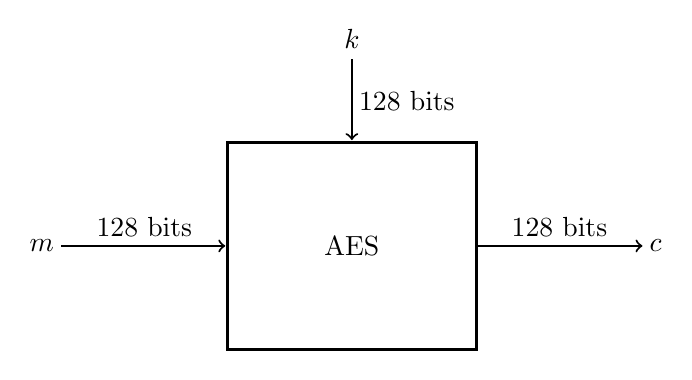
\begin{tikzpicture}[x=0.75pt,y=0.75pt,yscale=-1,xscale=1]

\draw  [line width=1.2]  (100,60) -- (220,60) -- (220,160) -- (100,160) -- cycle ;

\draw  [->]  (20,110) -- (99,110) ;
\draw  [->]  (220,110) -- (300,110) ;
\draw  [->]  (160,20) -- (160,59) ;

\draw (160,110) node   [align=left] {AES};
\draw (60,107) node [anchor=south] [inner sep=0.75pt]   [align=left] {$ 128$ bits};
\draw (260,107) node [anchor=south] [inner sep=0.75pt]   [align=left] {$ 128$ bits};
\draw (162,40) node [anchor=west] [inner sep=0.75pt]   [align=left] {$ 128$ bits};
\draw (18,110) node [anchor=east] [inner sep=0.75pt]    {$m$};
\draw (302,110) node [anchor=west] [inner sep=0.75pt]    {$c$};
\draw (160,16.6) node [anchor=south] [inner sep=0.75pt]    {$k$};


\end{tikzpicture}
  \caption{分组密码 AES}
  \label{fig:4-1}
\end{figure}

分组密码的安全性定义被表述为一种``黑盒测试"。大致思路是这样的:一个有效对手被赋予一个``黑盒",盒子里是 $\mathcal{X}$ 上的一个置换 $f$,它来自以下两个随机过程中的一个:
\begin{itemize}
	\item $f=E(k,\cdot)$,其中 $k$ 是一个随机选出的密钥,或者
	\item $f$ 是从 $\mathcal{X}$ 的\emph{所有}置换中随机均匀选出的一个真随机置换。
\end{itemize}
对手无法看到盒子的内部,但它可以用提问的方式来``探测"它:它可以给盒子一个值 $x\in\mathcal{X}$ 并得到一个 $y:=f(x)\in\mathcal{X}$。我们允许对手发起多次提问,而且我们允许它以任何它想要的方式选择问题;特别地,这些问题甚至可以以某种巧妙的方式依赖于盒子对之前的某个或某些问题的回答。安全性意味着,对手无论如何也无法得知盒子里的是哪种类型的函数——是随机密钥控制的分组密码,还是一个真的随机置换。换句话说,一个安全的分组密码应该与一个随机置换\textbf{在计算上不可区分}。

为了更正式地定义这一概念,我们首先引入一些表记符号。我们用:
\[
{\rm Perms}[\mathcal{X}]
\]
表示 $\mathcal{X}$ 上\emph{所有}置换的集合。需要注意,这是一个非常大的集合:
\[
\big\lvert
{\rm Perms}[\mathcal{X}]
\big\rvert
=|\mathcal{X}|!
\]
对于 AES 来说,$|\mathcal{X}|=2^{128}$,因此,置换的数量约为:
\[
\big\lvert
{\rm Perms}[\mathcal{X}]
\big\rvert
\approx 2^{2^{135}}
\]
而 $128$ 比特的 AES 密钥所定义置换的数量最多为 $2^{128}$。

和之前一样,为了定义安全性,我们引入一个攻击游戏。就如定义 PRG 的攻击游戏一样,这个攻击游戏也包含两个独立的实验。在这两个实验中,对手将遵循相同的协议,即它会向挑战者提交一连串的查询 $x_1,x_2,\dots$;挑战者则用 $f(x_i)$ 回应查询 $x_i$。在第一个实验中,$f=E(k,\cdot)$,其中 $k\in\mathcal{K}$ 是随机选出的一个元素;而在第二个实验中,$f$ 是从 ${\rm Perms}[\mathcal{X}]$ 中随机选出的一个置换。在每个实验中,挑战者都只能使用同一个 $f$ 来回应所有来自对手的查询。当对手决定终止对挑战者的查询时,它就会输出一个比特。

\begin{game}[分组密码]\label{game:4-1}
对于一个定义在 $(\mathcal{K},\mathcal{X})$ 上的给定分组密码 $(E,D)$ 和一个给定对手 $\mathcal{A}$,我们定义两个实验:实验 $0$ 和实验 $1$。对于 $b=0,1$,我们定义:

\noindent\textbf{实验 $b$:}
\begin{itemize}
	\item 挑战者按如下方式选择 $f\in{\rm Perms}[\mathcal{X}]$:
	
	\hspace*{26pt} 如果 $b=0$:随机选取 $k\overset{\rm R}\leftarrow\mathcal{K}$,令 $f\leftarrow E(k,\cdot)$;\\
	\hspace*{26pt} 如果 $b=1$:随机选取 $f\overset{\rm R}\leftarrow{\rm Perms}[\mathcal{X}]$。
	
	\item 对手向挑战者发起一系列查询。\\
	对于 $i=1,2,\dots$,第 $i$ 个查询是一个数据分组 $x_i\in\mathcal{X}$。\\
	挑战者计算 $y_i\leftarrow f(x_i)\in\mathcal{X}$,并将 $y_i$ 交给对手。
	\item 对手计算并输出一个比特 $\hat b\in\{0,1\}$。
\end{itemize}

对于 $b=0,1$,令 $W_b$ 为 $\mathcal{A}$ 在实验 $b$ 中输出 $1$ 的事件。我们将 $\mathcal{A}$ 就 $\mathcal{E}$ 的\textbf{优势}定义为:
\[
\mathrm{BC}\mathsf{adv}[\mathcal{A},\mathcal{E}]
:=
\big\lvert
\Pr[W_0]-\Pr[W_1]
\big\rvert
\]
最后,如果 $\mathcal{A}$ 最多发起 $Q$ 次查询,我们就称 $\mathcal{A}$ 就是一个 \textbf{$Q$ 次查询 BC 对手}。
\end{game}

图 \ref{fig:4-2} 展示了攻击游戏 \ref{game:4-1} 中的两个实验。

\begin{definition}[安全的分组密码]\label{def:4-1}
如果对于所有有效对手 $\mathcal{A}$,${\rm BC\mathsf{adv}}[\mathcal{A},\mathcal{E}]$ 的值都可忽略不计,那么分组密码 $\mathcal{E}$ 就是\textbf{安全的}。
\end{definition}

我们强调,挑战者在攻击游戏 \ref{game:4-1} 中的查询可以是\emph{自适应的(adaptive)};也就是说,对手不需要事先选择所有的查询;相对地,对手可以以某种巧妙的方式,根据挑战者之前的应答来炮制接下来的每个查询(见练习 \ref{exer:4-6})。

正如 \ref{subsec:2-2-5} 小节所讨论的,攻击游戏 \ref{game:4-1} 也可以被重构为一个``比特猜测"游戏,此时挑战者不再有两个独立的实验,而是随机选择 $b\in\{0,1\}$,然后针对对手 $\mathcal{A}$ 运行实验 $b$。在这个游戏中,我们记 $\mathcal{A}$ 的\emph{比特猜测优势}${\rm BC\mathsf{adv}}^*[\mathcal{A},\mathcal{E}]$ 为 $|\Pr[\hat b = b]-{1}/{2}|$。\ref{subsec:2-2-5} 小节的推广结论(即式 \ref{eq:2-11})在此依旧适用:
\begin{equation}
\mathrm{BC}\mathsf{adv}[\mathcal{A},\mathcal{E}]
=2\cdot
\mathrm{BC}\mathsf{adv}^*[\mathcal{A},\mathcal{E}]
\end{equation}

\begin{figure}[p!]
  \centering
  \tikzset{every picture/.style={line width=0.75pt}}     

\begin{tikzpicture}[x=0.75pt,y=0.75pt,yscale=-0.9,xscale=0.9]

\draw  [line width=1.2]  (0,0) -- (180,0) -- (180,250) -- (0,250) -- cycle ;
\draw  [line width=1.2]  (290,0) -- (410,0) -- (410,250) -- (290,250) -- cycle ;
\draw  [line width=1.2]  (0,300) -- (180,300) -- (180,550) -- (0,550) -- cycle ;
\draw  [line width=1.2]  (290,300) -- (410,300) -- (410,550) -- (290,550) -- cycle ;

\draw  [->]  (180,180) -- (290,180) ;
\draw  [->]  (290,220) -- (180,220) ;
\draw  [->]  (290,140) -- (180,140) ;
\draw  [->]  (180,480) -- (290,480) ;
\draw  [->]  (290,520) -- (180,520) ;
\draw  [->]  (290,440) -- (180,440) ;

\draw [dash pattern={on 4.5pt off 4.5pt}] [<-]  (243.7,172.35) .. controls (241.98,179.91) and (238.73,185) .. (235,185) .. controls (229.48,185) and (225,173.81) .. (225,160) .. controls (225,146.19) and (229.48,135) .. (235,135) .. controls (239.21,135) and (242.81,141.5) .. (244.29,150.71) ;

\draw [dash pattern={on 4.5pt off 4.5pt}] [<-] (243.7,472.35) .. controls (241.98,479.91) and (238.73,485) .. (235,485) .. controls (229.48,485) and (225,473.81) .. (225,460) .. controls (225,446.19) and (229.48,435) .. (235,435) .. controls (239.21,435) and (242.81,441.5) .. (244.29,450.71) ;

\draw (90,20) node   [align=left] {挑战者};
\draw (90,40) node   [align=left] {(实验 $ 0$)};
\draw (45,110) node [anchor=west] [inner sep=0.75pt]    {$k\overset{\mathrm{R}}{\leftarrow }\mathcal{K}$};
\draw (45,140) node [anchor=west] [inner sep=0.75pt]    {$y_{i}\leftarrow E( k,x_{i})$};
\draw (200,176.6) node [anchor=south] [inner sep=0.75pt]    {$y_{i}$};
\draw (235,216.6) node [anchor=south] [inner sep=0.75pt]    {$\hat{b} \in \{0,1\}$};
\draw (350,20) node    {$\mathcal{A}$};
\draw (90,320) node   [align=left] {挑战者};
\draw (90,340) node   [align=left] {(实验 $ 1$)};
\draw (350,320) node    {$\mathcal{A}$};
\draw (45,410) node [anchor=west] [inner sep=0.75pt]    {$f\overset{\mathrm{R}}{\leftarrow }\mathrm{Perm}[\mathcal{X}]$};
\draw (45,440) node [anchor=west] [inner sep=0.75pt]    {$y_{i}\leftarrow f( x_{i})$};
\draw (265,136.6) node [anchor=south] [inner sep=0.75pt]    {$x_{i} \in \mathcal{X}$};
\draw (200,476.6) node [anchor=south] [inner sep=0.75pt]    {$y_{i}$};
\draw (235,516.6) node [anchor=south] [inner sep=0.75pt]    {$\hat{b} \in \{0,1\}$};
\draw (265,436.6) node [anchor=south] [inner sep=0.75pt]    {$x_{i} \in \mathcal{X}$};


\end{tikzpicture}  
  \caption{攻击游戏 \ref{game:4-1}}
  \label{fig:4-2}
\end{figure}

\subsection{安全性的引申义}\label{subsec:4-1-1}

令 $\mathcal{E}=(E,D)$ 是一个定义在 $(\mathcal{K},\mathcal{X})$ 上的分组密码。为了进一步了解安全性的含义,我们下面讨论几个简单的结论。简单起见,我们假设 $|\mathcal{X}|$ 是大的(即超多项式的)。

\subsubsection{安全的分组密码是不可预测的}\label{subsubsec:4-1-1-1}

我们下面说明,如果密码 $\mathcal{E}$ 在定义 \ref{def:4-1} 的意义上是安全的,那么它一定是\emph{不可预测的},这意味着,每个有效对手赢得下面的\emph{预测游戏}的概率都可忽略不计。在这个游戏中,挑战者随机选择一个密钥 $k$,而对手提交一连串的查询 $x_1,\dots,x_Q$;对于对手的第 $i$ 次查询,挑战者以 $E(k,x_i)$ 作为应答。这些查询是自适应的,也就是说,对手的每个查询都可能取决于挑战者之前的应答。最后,挑战者会输出数对 $(x_{Q+1},y)$,其中 $x_{Q+1}\notin\{x_1,\dots,x_Q\}$。如果有 $y=E(k,x_{Q+1})$,我们就称对手赢得了这个游戏。

为了证明这一结论,我们不妨先假设 $\mathcal{E}$ 不是不可预测的,这就意味着,存在一个有效对手 $\mathcal{A}$,它能以不可忽略不计的概率 $p$ 赢得上述预测游戏。于是,我们可以利用 $\mathcal{A}$ 来打破 $\mathcal{E}$ 在定义 \ref{def:4-1} 意义上的安全性。为此,我们可以构造一个对手 $\mathcal{B}$,它一边进行攻击游戏 \ref{game:4-1},一边在上述预测游戏中扮演 $\mathcal{A}$ 的挑战者的角色。每当 $\mathcal{A}$ 发起查询 $x_i$ 时,对手 $\mathcal{B}$ 就将 $x_i$ 转发给自己在攻击游戏 \ref{game:4-1} 中的挑战者,然后得到一个应答 $y_i$,并将其传回给 $\mathcal{A}$。最后,当 $\mathcal{A}$ 输出 $(x_{Q+1},y)$ 时,对手 $\mathcal{B}$ 就将 $x_{Q+1}$ 提交给自己的挑战者,得到 $y_{Q+1}$。如果 $y=y_{Q+1}$,$\mathcal{B}$ 就输出 $1$,否则就输出 $0$。

一方面,如果 $\mathcal{B}$ 的挑战者运行的是实验 $0$,$\mathcal{B}$ 就会以概率 $p$ 输出 $1$。另一方面,如果 $\mathcal{B}$ 的挑战者运行的是实验 $1$,$\mathcal{B}$ 就会以可忽略不计的概率 $\epsilon$ 输出 $1$(这是因为我们假设 $|\mathcal{X}|$ 是超多项式的)。这意味着 $\mathcal{B}$ 在攻击游戏 \ref{game:4-1} 中的优势是 $|p-\epsilon|$,而这个值是不可忽略不计的。

\subsubsection{不可预测性意味着对密钥恢复的安全性}\label{subsubsec:4-1-1-2}

我们下面说明,如果 $\mathcal{E}$ 是不可预测的,那么它\emph{对密钥恢复攻击是安全的},这意味着每个有效对手赢得下面的\emph{密钥恢复游戏}的概率都可忽略不计。在这个游戏中,对手与挑战者的交互方式与上面的预测游戏完全一样,区别只是在最后,对手需要输出一个候选密钥 $\mathpzc{k}\in\mathcal{K}$。如果 $\mathpzc{k}=k$,我们就称对手赢得了该游戏。

为了证明这一结论,我们不妨先假设 $\mathcal{E}$ 对密钥恢复攻击不安全,这就意味着,存在一个有效对手 $\mathcal{A}$,它能以不可忽略不计的概率 $p$ 赢得密钥恢复游戏。于是,我们可以使用 $\mathcal{A}$ 来建立一个有效对手 $\mathcal{B}$,它能以至少 $p$ 的概率赢得上面的预测游戏。对手 $\mathcal{B}$ 只需要运行 $\mathcal{A}$ 的攻击,然后在 $\mathcal{A}$ 输出 $\mathpzc{k}$ 的时侯任意选择一个 $x_{Q+1}\notin\{x_1,\dots,x_Q\}$,计算 $y\leftarrow E(\mathpzc{k},x_{Q+1})$ 并输出 $(x_{Q+1},y)$。

不难看出,如果 $\mathcal{A}$ 能够赢得密钥恢复游戏,$\mathcal{B}$ 就能够赢得预测游戏。

\subsubsection{密钥空间大小和穷举搜索攻击}

结合上面的两个结论,我们可以知道:如果 $\mathcal{E}$ 是一个安全的分组密码,那么它对密钥恢复攻击也一定是安全的。此外,如果 $\mathcal{E}$ 对密钥恢复攻击是安全的,那么 $|\mathcal{K}|$ 一定是大的。

下面的这种方法可以证明这个结论。任何一个对手只要从密钥空间 $\mathcal{K}$ 中随机选取一个 $\mathpzc{k}$,就能以 ${1}/{|\mathcal{K}|}$ 的概率赢得密钥恢复游戏。而如果 $|\mathcal{K}|$ 不是超多项式的,${1}/{|\mathcal{K}|}$ 就不可忽略不计。因此,当 $|\mathcal{K}|$ 不是超多项式的时候,这个简单的密钥猜测对手就能以不可忽略不计的概率赢得密钥恢复游戏。

我们也可以通过另一种称为\emph{穷举搜索攻击(exhaustive-search attack)}的方式来用运行时间换取成功概率。在这种攻击中,我们的对手在密钥恢复游戏中进行一些任意的查询 $x_1,\dots,x_Q$,并获得应答 $y_1,\dots,y_Q$。我们可以认为——至少从启发式的角度来看——假设 $|\mathcal{X}|\geq|\mathcal{K}|$,并且 $|\mathcal{X}|$ 是超多项式的,对于相当小的 $Q$ 值(事实上 $Q=2$),仅有一个密钥 $k$ 能够以与 $1$ 相差可不略不计的概率使得:
\begin{equation}\label{eq:4-2}
y_i=E(k,x_i),
\;\;
i=1,\dots,Q
\end{equation}
因此,我们的对手只需尝试所有可能的密钥,必然能够找到一个满足式 \ref{eq:4-2} 的密钥 $k$。如果只有一个符合条件的密钥,那么对手找到的密钥就会是挑战者选择的密钥,而对手将赢得游戏。因此,对手能以与 $1$ 相差可忽略不计的概率赢得密钥恢复游戏,但是它的运行时间是 $|\mathcal{K}|$ 的线性函数。

这种时间/优势的权衡很容易被推广。事实上,考虑一个随机选择 $t$ 个密钥的对手,它测试每个密钥是否满足式 \ref{eq:4-2}。该对手的运行时间是 $t$ 的线性函数,并且它能以 $\approx{t}/{|\mathcal{K}|}$ 的概率赢得密钥恢复游戏。

我们将在 \ref{subsec:4-2-2} 小节中描述一些现实世界中的穷举搜索攻击。我们将在 \ref{subsec:4-7-2} 小节中对穷举搜索进行详细的处理,特别是,我们届时将证明上面所使用的启发式假设,即最多仅有一个密钥能够以高概率满足式 \ref{eq:4-2}。

因此,很显然地,我们如果想要保证一个分组密码是安全的,就必须赋予它一个大的密钥空间,目的是使其能够抵抗密钥恢复攻击。

\subsection{随机置换的有效实现}\label{subsec:4-1-2}

请注意,在攻击游戏 \ref{game:4-1} 的实验 $1$ 中,挑战者的协议并不是很高效,因为它需要构造一个\emph{极大的}随机对象。事实上,仅仅写下 ${\rm Perms}[\mathcal{X}]$ 中的一个元素就需要大约 $|\mathcal{X}|\log_2|\mathcal{X}|$ 个比特。对于 AES 来说,$|\mathcal{X}|=2^{128}$,这意味着大约需要 $10^{40}$ 个比特!

虽然从纯粹的定义角度来看,这好像并不是一个问题。但考虑到审美和技术实现,如果能有一个更高效的实现就更好了。事实上,我们可以通过一个``惰性"的方式来实现 $f$。具体来说,挑战者可以通过跟踪输入/输出对 $(x_i,y_i)$ 来表示随机置换 $f$。当挑战者收到第 $i$ 个查询 $x_i$ 时,它会测试是否存在某个 $j<i$ 能使得 $x_i=x_j$;如果确实存在这样的 $j$,它就令 $y_i\leftarrow y_j$(这保证挑战者实现的是一个函数);否则,它就从 $\mathcal{X}\setminus\{y_1,\dots,y_{i-1}\}$ 中随机选出一个 $y_i$(这确保该函数是一个置换);最后,它将 $y_i$ 发送给对手。我们可以把挑战者的逻辑表述如下:

\vspace*{10pt}

\hspace*{5pt} 当从对手 $\mathcal{A}$ 处收到第 $i$ 个查询 $x_i\in\mathcal{X}$ 时:\\
\hspace*{50pt} 如果存在某个 $j<i$ 使得 $x_i=x_j$ 成立:\\
\hspace*{75pt} 则令 $y_i\leftarrow y_j$\\
\hspace*{75pt} 否则令 $y_i\overset{\rm R}\leftarrow\mathcal{X}\setminus\{y_1,\dots,y_{i-1}\}$\\
\hspace*{50pt} 将 $y_i$ 发送给 $\mathcal{A}$。

\vspace*{10pt}

\noindent
为了使这个实现尽可能快,我们可以使用一个恰当的字典数据结构(比如哈希表、搜索前缀树、平衡树等)来实现对``是否存在某个 $j<i$ 使得 $x_i=x_j$ 成立"的检验。假设可以有效地生成 $\mathcal{X}$ 中的随机元素,那么实现 ``$y_i\overset{R}\leftarrow\mathcal{X}\setminus\{y_1,\dots,y_{i-1}\}$"这一步的方法如下:

\vspace*{10pt}

\hspace*{5pt} 重复 $y\overset{\rm R}\leftarrow\mathcal{X}$,直至 $y\notin\{y_1,\dots,y_{i-1}\}$\\
\hspace*{26pt} 令 $y_i\leftarrow y$

\vspace*{10pt}

\noindent
同样,我们可以使用适当的字典数据结构来检验``$y\notin\{y_1,\dots,y_{i-1}\}$"是否成立。当 $i<{|\mathcal{X}|}/{2}$ 时,预期上只需要运行两次迭代即可找到满足要求的 $y_i$。

一种理解这个实现的方式是,实验 $1$ 中的挑战者就是一个``黑盒",但盒子里有一个\textbf{忠实的侏儒(faithful gnome)},它的工作就是维护一张表示随机置换 $f$ 的输入/输出表,如图 \ref{fig:4-3} 所示。

\begin{figure}
  \centering
  

\tikzset{every picture/.style={line width=0.75pt}} %set default line width to 0.75pt        

\begin{tikzpicture}[x=0.75pt,y=0.75pt,yscale=-1,xscale=1]
%uncomment if require: \path (0,263); %set diagram left start at 0, and has height of 263

\node at (165,175) {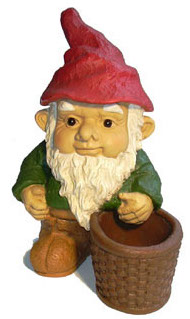
\includegraphics[width=60pt]{figures/chapter4/gnome.jpeg}};

%Shape: Rectangle [id:dp721778058251819] 
\draw  [line width=1.2]  (120,0) -- (320,0) -- (320,250) -- (120,250) -- cycle ;
%Right Arrow [id:dp5887472607772757] 
\draw  [line width=1.2]  (0,60) -- (75.25,60) -- (75.25,45) -- (100,75) -- (75.25,105) -- (75.25,90) -- (0,90) -- cycle ;
%Straight Lines [id:da03851464693257456] 
\draw    (180,50) -- (300,50) ;
%Straight Lines [id:da49911218049186523] 
\draw    (240,30) -- (240,130) ;
%Right Arrow [id:dp9356939686312407] 
\draw  [line width=1.2]  (100,200) -- (25,200) -- (25,215) -- (0,185) -- (25,155) -- (25,170) -- (100,170) -- cycle ;

% Text Node
\draw (210,40) node    {$x$};
% Text Node
\draw (270,40) node    {$f(x)$};
% Text Node
\draw (210,60) node    {\texttt{00101}};
% Text Node
\draw (210,80) node    {\texttt{11111}};
% Text Node
\draw (210,100) node    {\texttt{10111}};
% Text Node
\draw (210,120) node    {\texttt{00011}};
% Text Node
\draw (270,60) node    {\texttt{10101}};
% Text Node
\draw (270,80) node    {\texttt{01110}};
% Text Node
\draw (270,100) node    {\texttt{01011}};
% Text Node
\draw (270,120) node    {\texttt{10001}};
% Text Node
\draw (50,75) node    {$x$};
% Text Node
\draw (50,185) node    {$f( x)$};



\end{tikzpicture}
  \caption{一个忠实的侏儒实现了随机置换$f$}
  \label{fig:4-3}
\end{figure}

\subsection{强安全的分组密码}\label{subsec:4-1-3}

请注意,在攻击游戏 \ref{game:4-1} 中,解密算法 $D$ 从未被使用过。事实上,我们可以定义一个攻击游戏来给出一个更强的安全概念,在这个游戏中,对手被允许向挑战者发起两种类型的查询:
\begin{itemize}
	\item \textbf{前向查询}:对手向挑战者发送一个值 $x_i\in\mathcal{X}$,挑战者以 $y_i:=f(x_i)$ 应答对手;
	\item \textbf{反向查询}:对手向挑战者发送一个值 $y_i\in\mathcal{X}$,挑战者以 $x_i:=f^{-1}(y_i)$ 应答对手(在攻击游戏的实验$0$中,这是使用算法$D$完成的)。
\end{itemize}
接下来,我们可以为这个攻击游戏定义一个相应的优势。如果对于所有有效对手,这个优势都是可忽略不计的,我们就称这个分组密码是\textbf{强安全(strongly secure)}的。我们把这个定义的细节留给读者去解决(见练习 \ref{exer:4-9})。除了在后续章节中的一个应用实例(练习 \ref{exer:9-12})之外,我们不会在本文中使用这个概念。

\subsection{直接使用分组密码进行加密}\label{subsec:4-1-4}

既然分组密码是一种特殊的密码,我们当然可以考虑直接使用它进行加密。问题是,一个安全的分组密码是否也是语义安全的?

只要消息空间和数据分组空间相等,上面的问题的答案就是``是的"。下面的定理 \ref{theo:4-1} 将会指出这一点。然而在实践中,分组密码的数据分组非常短,正如我们之前提到的,AES 的数据分组只有 128 比特。如果我们想加密更长的消息,一个自然的想法是将一个长消息分解成一连串的数据分组,并对每个数据分组单独进行加密。这种使用分组密码来加密长消息的方法被称为\textbf{电子密码本模式 (electronic codebook mode, ECB)}。

更确切地说,假设 $\mathcal{E}=(E,D)$ 是一个定义在 $(\mathcal{K},\mathcal{X})$ 上的分组密码。对于任意多项式边界的 $\ell\geq1$,我们可以定义一个 $(\mathcal{K},\mathcal{X}^{\leq\ell},\mathcal{X}^{\leq\ell})$ 上的密码 $\mathcal{E}'=(E',D')$ 如下:
\begin{itemize}
	\item 对于 $k\in\mathcal{K}$ 和 $m\in\mathcal{X}^{\leq\ell}$,如果记 $v:=|m|$,我们定义:
	\[
    E'(k,m)=(E(k,m[0]),\dots,E(k,m[v-1]))
    \]
	\item 对于 $k\in\mathcal{K}$ 和 $c\in\mathcal{X}^{\leq\ell}$,如果记 $v:=|c|$,我们定义:
	\[
	D'(k,c)=(D(k,c[0]),\dots,D(k,c[v-1]))
	\]
\end{itemize}
图 \ref{fig:4-4} 展示了加解密的工作逻辑。我们称 $\mathcal{E}'$ 为\textbf{由 $\mathcal{E}$ 派生的 $\ell$ 次 ECB 密码 ($\ell$-wise ECB cipher derived from $\mathcal{E}$)}。

\begin{figure}
  \centering
  \subfigure[加密]{\tikzset{every picture/.style={line width=0.75pt}}

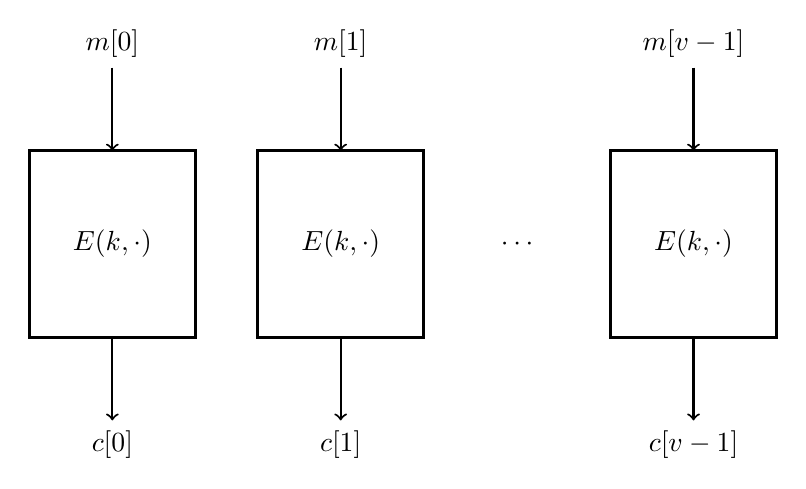
\begin{tikzpicture}[x=0.75pt,y=0.75pt,yscale=-1,xscale=1]

\draw  [line width=1.2]  (0,80) -- (80,80) -- (80,170) -- (0,170) -- cycle ;
\draw  [line width=1.2]  (110,80) -- (190,80) -- (190,170) -- (110,170) -- cycle ;
\draw  [line width=1.2]  (280,80) -- (360,80) -- (360,170) -- (280,170) -- cycle ;

\draw  [->]  (40,40) -- (40,80) ;
\draw  [->]  (40,170) -- (40,210) ;
\draw  [->]  (150,40) -- (150,80) ;
\draw  [->]  (150,170) -- (150,210) ;
\draw  [->]  (320,40) -- (320,80) ;
\draw  [->]  (320,170) -- (320,210) ;

\draw (40,125) node    {$E( k,\cdot )$};
\draw (40,36.6) node [anchor=south] [inner sep=0.75pt]    {$m[ 0]$};
\draw (40,213.4) node [anchor=north] [inner sep=0.75pt]    {$c[ 0]$};
\draw (150,125) node    {$E( k,\cdot )$};
\draw (150,36.6) node [anchor=south] [inner sep=0.75pt]    {$m[ 1]$};
\draw (150,213.4) node [anchor=north] [inner sep=0.75pt]    {$c[ 1]$};
\draw (320,125) node    {$E( k,\cdot )$};
\draw (320,36.6) node [anchor=south] [inner sep=0.75pt]    {$m[ v-1]$};
\draw (320,213.4) node [anchor=north] [inner sep=0.75pt]    {$c[ v-1]$};
\draw (235,125) node    {$\cdots $};


\end{tikzpicture}}
  
  \,
  
  \,
  
  \subfigure[解密]{\tikzset{every picture/.style={line width=0.75pt}}      

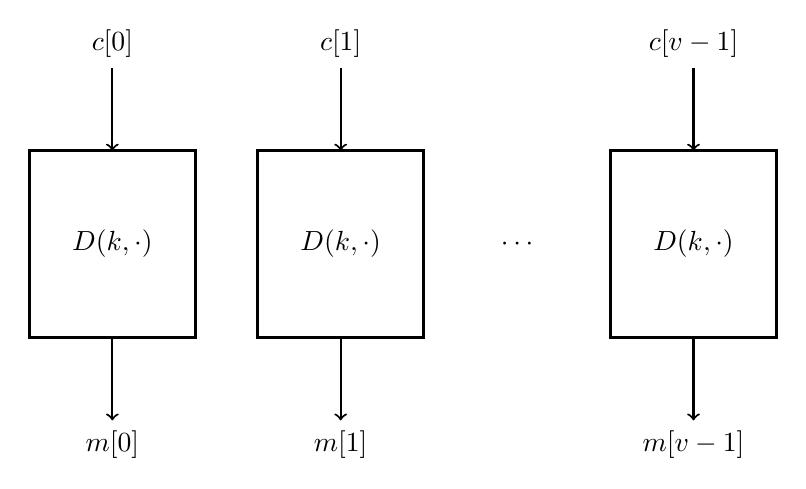
\begin{tikzpicture}[x=0.75pt,y=0.75pt,yscale=-1,xscale=1]


\draw  [line width=1.2]  (0,80) -- (80,80) -- (80,170) -- (0,170) -- cycle ;
\draw  [line width=1.2]  (110,80) -- (190,80) -- (190,170) -- (110,170) -- cycle ;
\draw  [line width=1.2]  (280,80) -- (360,80) -- (360,170) -- (280,170) -- cycle ;

\draw  [->]  (40,40) -- (40,80) ;
\draw  [->]  (40,170) -- (40,210) ;
\draw  [->]  (150,40) -- (150,80) ;
\draw  [->]  (150,170) -- (150,210) ;
\draw  [->]  (320,40) -- (320,80) ;
\draw  [->]  (320,170) -- (320,210) ;

\draw (40,125) node    {$D( k,\cdot )$};
\draw (40,36.6) node [anchor=south] [inner sep=0.75pt]    {$c[ 0]$};
\draw (40,213.4) node [anchor=north] [inner sep=0.75pt]    {$m[ 0]$};
\draw (150,125) node    {$D( k,\cdot )$};
\draw (150,36.6) node [anchor=south] [inner sep=0.75pt]    {$c[ 1]$};
\draw (150,213.4) node [anchor=north] [inner sep=0.75pt]    {$m[ 1]$};
\draw (320,125) node    {$D( k,\cdot )$};
\draw (320,36.6) node [anchor=south] [inner sep=0.75pt]    {$c[ v-1]$};
\draw (320,213.4) node [anchor=north] [inner sep=0.75pt]    {$m[ v-1]$};
\draw (235,125) node    {$\cdots $};


\end{tikzpicture}}
  \caption{ECB模式的加密与解密}
  \label{fig:4-4}
\end{figure}

ECB 密码与例 \ref{exmp:2-3} 和例 \ref{exmp:2-6} 中讨论的置换密码有非常密切的关系。主要区别在于,我们现在不是从 $\mathcal{X}$ 上所有可能的置换中完全随机地选择一个,而是在小得多的置换 $\{E(k,\cdot):k\in\mathcal{K}\}$ 中选择。另一个不太重要的区别是,在例 \ref{exmp:2-3} 中,我们定义的置换密码拥有定长的消息空间(这实际上只是一个任意的选择,因为我们也可以将置换密码定义在变长的消息空间上),而 ECB 密码的消息空间可以是变长的。除此以外,在例 \ref{exmp:2-3} 中,我们举了一个大小为 $27$ 的置换密码的例子,但如果我们使用像 AES 这样的分组长度为 $128$ 比特的密码,其``字母表"要大得多得多,事实上有 $2^{128}$ 那么大。尽管存在如此多的差异,例 \ref{exmp:2-6} 中讨论的置换密码的一些缺陷在 ECB 密码中也同样存在。下面我们举个例子。如果对两条消息 $m_0,m_1\in\mathcal{M}^2$ 进行 ECB 加密,其中 $m_0$ 由两个相同的分组组成(即 $m_0[0]=m_0[1]$),而 $m_1$ 由两个不同的分组组成(即 $m_1[0]\neq m_1[1]$),那么对手很容易就能区分出这两条消息的加密结果。单只因为这个原因,\emph{ECB 密码就不符合我们对语义安全的定义,因此,我们强烈反对将它作为加密方案使用}。

图 \ref{fig:4-5} 以图像的方式表现了这种能够轻易分辨相同明文分组的能力。这里,图像数据使用 ECB 模式加密,每个数据分组都来自对明文中小像素点的编码。由于相同的像素块会被映射到相同的密文上,所以原始图片中相同的像素在密文中也是相同的,我们可以从密文中依稀看到明文的轮廓。

但是请注意,也有一些例 \ref{exmp:2-6} 中讨论的缺陷在这里并不直接适用。假设我们在加密一个 ASCII 编码的文本。如果分组大小是 $128$ 比特,那么每个字符通常会被编码为一个字节,这样一个分组就由 $16$ 个字符组成。这时对手就无法像例 \ref{exmp:2-6} 中那样轻易地找到个别重复字符的位置了。

\vspace{10pt}

在本节的最后,我们将要表明,如果消息空间被限制为\emph{各不相同的}数据分组的序列,那么 ECB 模式实际上是安全的。这对于单个分组加密的特殊情况也是适用的。例如,假设我们使用的是 AES,它有 $128$ 比特的数据分组。那么,我们可以从每个数据分组中分配出 $32$ 比特作为计数器,并将剩余的 $96$ 比特作为承载消息的比特。有了这样的策略,我们可以将任何长达 $2^{32}\cdot 96$ 比特的消息编码为一串各不相同的数据分组。当然,这种策略的缺点是密文会比明文长 $33\%$。

\begin{figure}
  \centering
  \subfigure[明文]{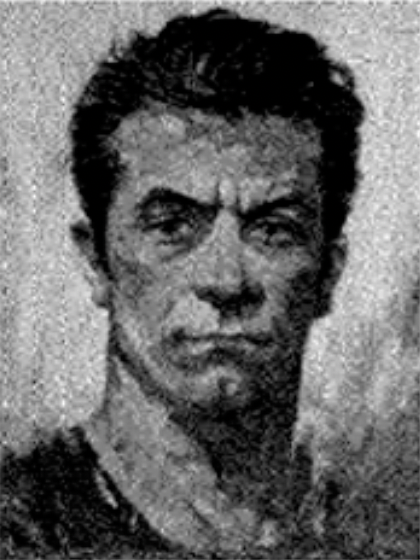
\includegraphics[width=0.21\linewidth]{figures/chapter4/fig5-a.png}}
  \quad\quad\quad\quad\quad
  \subfigure[使用AES在ECB模式下加密明文]{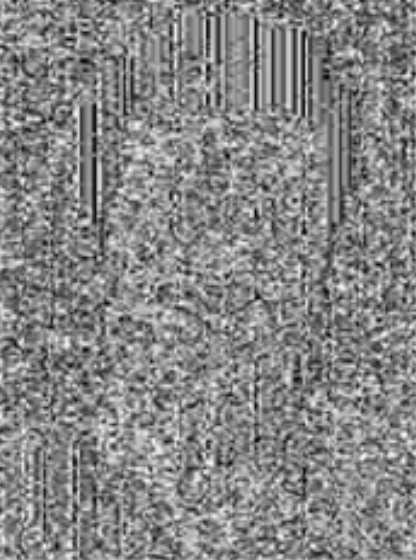
\includegraphics[width=0.21\linewidth]{figures/chapter4/fig5-b.png}}
  \caption{ECB模式中的加密}
  \label{fig:4-5}
\end{figure}

\begin{theorem}\label{theo:4-1}
令 $\mathcal{E}=(E,D)$ 是一个分组密码,$\ell\geq1$ 是任意多项式边界的值,令 $\mathcal{E}'=(E',D')$ 是由 $\mathcal{E}$ 派生的 $\ell$ 次 ECB 密码,但其消息空间被限制为最多 $\ell$ 个各不相同的数据分组的所有可能序列。如果 $\mathcal{E}$ 是一个安全的分组密码,那么 $\mathcal{E}'$ 就是一个语义安全的密码。
\begin{quote}
特别地,对于每个就 $\mathcal{E}'$ 进行攻击游戏 \ref{game:2-1} 的 SS 对手 $\mathcal{A}$,都存在一个就 $\mathcal{E}$ 进行攻击游戏 \ref{game:4-1} 的 BC 对手 $\mathcal{B}$,其中 $\mathcal{B}$ 是一个围绕 $\mathcal{A}$ 的基本包装器,满足:
\end{quote}
\begin{equation}\label{eq:4-3}
{\rm SS\mathsf{adv}}[\mathcal{A},\mathcal{E}']=2\cdot{\rm BC\mathsf{adv}}[\mathcal{B},\mathcal{E}]
\end{equation}
\end{theorem}

\begin{proof}[证明思路]
基本思想是,如果对手被赋予了一条消息的加密,而该消息是一串各不相同的数据分组,那么对手能看到的实际上也只是一个随机数据分组的序列(无替换采样)。
\end{proof}

\begin{proof}
如果 $\mathcal{E}$ 定义在 $(\mathcal{K},\mathcal{X})$ 上,令 $\mathcal{X}_*^{\leq\ell}$ 表示 $\mathcal{X}$ 中由最多 $\ell$ 个不同元素所组成的所有序列的集合。

令 $\mathcal{A}$ 是一个有效对手,它像攻击游戏 \ref{game:2-1} 中那样攻击 $\mathcal{E}'$。我们的目标是,假设 $\mathcal{E}$ 是一个安全的分组密码,证明 ${\rm SS\mathsf{adv}}[\mathcal{A},\mathcal{E}']$ 是可忽略不计的。使用语义安全攻击游戏的比特猜测版本更加方便。我们试图证明:
\begin{equation}\label{eq:4-4}
{\rm SS\mathsf{adv}}^*[\mathcal{A},\mathcal{E}']={\rm BC\mathsf{adv}}[\mathcal{B},\mathcal{E}]
\end{equation}
对于某个有效对手 $\mathcal{B}$ 成立。那么根据定理 \ref{theo:2-10},我们就能得到式 \ref{eq:4-3}。

所以,考虑对手 $\mathcal{A}$ 在攻击游戏 \ref{game:2-1} 的比特猜测版本中对 $\mathcal{E}'$ 的攻击。在这个游戏中,$\mathcal{A}$ 向挑战者发送两条长度相同的消息 $m_0,m_1$,然后挑战者选择一个随机密钥 $k$ 和一个随机比特 $b$,并用 $k$ 加密 $m_b$,将得到的密文 $c$ 交给 $\mathcal{A}$;最后,$\mathcal{A}$ 输出一个比特 $\hat b$。如果 $\hat b=b$,则对手 $\mathcal{A}$ 赢得游戏。

挑战者在该游戏中的逻辑可以表示如下:

\vspace*{10pt}

\hspace*{5pt} 当从对手 $\mathcal{A}$ 处收到消息 $m_0,m_1\in\mathcal{X}_*^{\leq\ell}$ 时,记 $v:=|m_0|=|m_1|$:\\
\hspace*{50pt} 选取 $b\overset{\rm R}\leftarrow\{0,1\}$\\
\hspace*{50pt} 选取 $k\overset{\rm R}\leftarrow\mathcal{K}$\\
\hspace*{50pt} 令 $c\leftarrow(E(k,m_b[0]),\dots,E(k, m_b[v-1]))$\\
\hspace*{50pt} 将 $c$ 发送给 $\mathcal{A}$。

\vspace*{10pt}

我们将该游戏称作\textbf{游戏 $\mathbf{0}$}。我们下面还将定义游戏 $1$ 和游戏 $2$。对于 $j=0,1,2$,我们定义 $W_j$ 为 $\mathcal{A}$ 在游戏 $j$ 中输出的 $\hat b=b$ 的事件。根据定义,我们有:
\begin{equation}\label{eq:4-5}
\mathrm{SS}\mathsf{adv}^*[\mathcal{A},\mathcal{E}']
=
|\Pr[W_0]-{1}/{2}|
\end{equation}

\noindent
\textbf{游戏 $\mathbf{1}$}。该游戏与游戏 $0$ 基本相同,只是现在,挑战者用一个随机的 $f\in{\rm Perms}[\mathcal{X}]$ 代替 $E(k,\cdot)$。我们的挑战者现在看起来是这样的:

\vspace*{10pt}

\hspace*{5pt} 当从对手 $\mathcal{A}$ 处收到消息 $m_0,m_1\in\mathcal{X}_*^{\leq\ell}$ 时,记 $v:=|m_0|=|m_1|$:\\
\hspace*{50pt} 选取 $b\overset{\rm R}\leftarrow\{0,1\}$\\
\hspace*{50pt} 选取 $f\overset{\rm R}\leftarrow{\rm Perms}[\mathcal{X}]$\\
\hspace*{50pt} 令 $c\leftarrow(f(m_b[0]),\dots,f(m_b[v-1]))$\\
\hspace*{50pt} 将 $c$ 发送给 $\mathcal{A}$。

\vspace*{10pt}

直观地说,$\mathcal{E}$ 是一个安全的分组密码的事实意味着,对手应该注意不到这个变化。为了严格地证明这一点,我们下面展示,如何构建一个分组密码对手 $\mathcal{B}$,使得它是一个围绕 $\mathcal{A}$ 的基本包装器,且满足:
\begin{equation}\label{eq:4-6}
\big\lvert
\Pr[W_0]-\Pr[W_1]
\big\rvert
=\mathrm{BC}\mathsf{adv}[\mathcal{B},\mathcal{E}]
\end{equation}

$\mathcal{B}$ 的设计直接来自于游戏 $0$ 和 $1$ 的逻辑。对手 $\mathcal{B}$ 就 $\mathcal{E}$ 进行攻击游戏 \ref{game:4-1},其工作原理如下:
\begin{quote}
记 $f$ 为 $\mathcal{B}$ 的分组密码挑战者在攻击游戏 \ref{game:4-1} 中选择的函数。我们让 $\mathcal{B}$ 扮演 $\mathcal{A}$ 的挑战者的角色,其工作逻辑如下:

\vspace*{5pt}

\hspace*{20pt} 当从对手 $\mathcal{A}$ 处收到消息 $m_0,m_1\in\mathcal{X}_*^{\leq\ell}$ 时,记 $v:=|m_0|=|m_1|$:\\
\hspace*{50pt} 选取 $b\overset{\rm R}\leftarrow\{0,1\}$\\
\hspace*{50pt} 令 $c\leftarrow(f(m_b[0]),\dots,f(m_b[v-1]))$\\
\hspace*{50pt} 将 $c$ 发送给 $\mathcal{A}$。

\vspace*{5pt}

请注意,$\mathcal{B}$ 通过查询它自己的分组密码挑战者来计算 $f(m_b[0]),\dots,f(m_b[v-1])$。最后,当 $\mathcal{A}$ 输出一个比特 $\hat b$ 时,$\mathcal{B}$ 输出 $\delta(\hat b,b)$,其中 $\delta$ 的定义见式 \ref{eq:3-7}。
\end{quote}

\vspace{8pt}

\noindent
显然,当 $\mathcal{B}$ 处于其攻击游戏的实验 $0$ 时,它会以 $\Pr[W_0]$ 的概率输出 $1$。而当 $\mathcal{B}$ 处于其攻击游戏的实验 $1$ 时,它会以 $\Pr[W_1]$ 的概率输出 $1$。这样,我们就能得到式 \ref{eq:4-6}。

\vspace{8pt}

\noindent
\textbf{游戏 $\mathbf{2}$}。
现在,我们重写游戏 $1$ 中的挑战者,让其使用我们在 \ref{subsec:4-1-2} 小节中讨论的``忠实的侏儒"来实现随机置换。$m_0$ 和 $m_1$ 的每条消息都需要由各不相同的数据分组组成(我们的挑战者不需要验证这一点),因此我们的侏儒的工作很容易:它甚至不需要看输入数据分组,因为这些数据分组被确保是各不相同的;然而,它仍然需要确保它产生的输出分组是各不相同的。

我们可以把我们的挑战者的逻辑表述如下:

\vspace*{10pt}

\hspace*{5pt} 选取 $y_0\overset{\rm R}\leftarrow\mathcal{X}$,$y_1\overset{\rm R}\leftarrow\mathcal{X}\setminus\{y_0\}$,$\dots$,$y_{\ell-1}\overset{\rm R}\leftarrow\mathcal{X}\setminus\{y_0,\dots,y_{\ell-2}\}$\\
\hspace*{26pt} 当从对手 $\mathcal{A}$ 处收到消息 $m_0,m_1\in\mathcal{X}_*^{\leq\ell}$ 时,记 $v:=|m_0|=|m_1|$:\\
\hspace*{50pt} 选取 $b\overset{\rm R}\leftarrow\{0,1\}$\\
\hspace*{50pt} 令 $c\leftarrow(y_0,\dots,y_{v-1})$\\
\hspace*{50pt} 将 $c$ 发送给 $\mathcal{A}$。

\vspace*{10pt}

由于我们的侏儒是忠实的,我们有:
\begin{equation}\label{eq:4-7}
\Pr[W_1]=\Pr[W_2]
\end{equation}
此外,我们声称:
\begin{equation}\label{eq:4-8}
\Pr[W_2]={1}/{2}
\end{equation}
这来自这样一个事实:在游戏 $2$ 中,对手的输出 $\hat b$ 是它自己的随机选择,以及 $y_0,\dots,y_{\ell-1}$ 的一个函数。由于这些值(根据定义)与 $b$ 无关,因此 $\hat b$ 和 $b$ 是相互独立的。所以式 \ref{eq:4-8} 成立。

综合式 \ref{eq:4-5},式 \ref{eq:4-6},式 \ref{eq:4-7} 和式 \ref{eq:4-8},我们就能得到式 \ref{eq:4-4},因此定理 \ref{theo:4-1} 得证。
\end{proof}

\subsection{数学细节}\label{subsec:4-1-5}

和之前一样,我们下面讨论一些之前被忽略了的数学细节。

由于分组密码只是一种特殊的密码,所以关于分组密码的定义,其实没有什么是 \ref{sec:2-3} 节中没有交代的。像往常一样,定义 \ref{def:4-1} 需要被正确地解释。首先,在攻击游戏 \ref{game:4-1} 中,我们要理解,对于安全参数 $\lambda$ 的每个值,我们都会得到一个不同的概率空间,它由挑战者的随机选择和对手的随机选择共同决定。其次,挑战者会产生一个系统参数 $\Lambda$,并在游戏一开始就将其发送给对手。第三,优势 ${\rm BC\mathsf{adv}}[\mathcal{B},\mathcal{E}]$ 是安全参数 $\lambda$ 的一个函数,安全性则意味着它是一个可忽略不计函数。
\section{在实践中构建分组密码}\label{sec:4-2}

分组密码是密码学中的一个基本原语,许多其他系统都是基于它建立的。几乎所有在实践中使用的分组密码都使用了相同的基本框架,称为\textbf{迭代密码 (iterated cipher)}范式。为了构建一个迭代分组密码,设计者需要做出以下两个抉择:
\begin{itemize}
	\item 首先,他需要选择一个简单的分组密码 $\mathcal{\hat E}:=(\hat E,\hat D)$,它本身显然是不安全的。我们称 $\mathcal{\hat E}$ 为\textbf{轮密码 (round cipher)}。
	\item 其次,他还需要选择一个简单(但不一定安全)的 PRG $G$,用来将密钥 $k$ 扩展为 $\mathcal{\hat E}$ 的 $d$ 个密钥 $k_1,\dots,k_d$。我们称 $G$ 为\textbf{密钥扩展函数 (key expansion function)}。
\end{itemize}
一旦做出这两个选择,迭代分组密码 $\mathcal{E}$ 就完全确定下来了。加密算法 $E(k,x)$ 的工作原理如下(另见图 \ref{fig:4-6}):

\begin{figure}
  \centering
  \tikzset{every picture/.style={line width=0.75pt}} 

\begin{tikzpicture}[x=0.75pt,y=0.75pt,yscale=-1,xscale=1]


\draw  [draw opacity=0][fill={rgb, 255:red, 155; green, 155; blue, 155 }  ,fill opacity=0.6 ] (95,60) -- (240,20) -- (300,20) -- (445,60) -- cycle ;

\draw  [fill={rgb, 255:red, 255; green, 255; blue, 255 }  ,fill opacity=1 ][line width=1.2] [general shadow={fill=black,shadow xshift=2.25pt,shadow yshift=-2.25pt}] (60,150) -- (120,150) -- (120,210) -- (60,210) -- cycle ;
\draw  [fill={rgb, 255:red, 255; green, 255; blue, 255 }  ,fill opacity=1 ][line width=1.2] [general shadow={fill=black,shadow xshift=2.25pt,shadow yshift=-2.25pt}] (160,150) -- (220,150) -- (220,210) -- (160,210) -- cycle ;
\draw  [fill={rgb, 255:red, 255; green, 255; blue, 255 }  ,fill opacity=1 ][line width=1.2] [general shadow={fill=black,shadow xshift=2.25pt,shadow yshift=-2.25pt}] (260,150) -- (320,150) -- (320,210) -- (260,210) -- cycle ;
\draw  [fill={rgb, 255:red, 255; green, 255; blue, 255 }  ,fill opacity=1 ][line width=1.2] [general shadow={fill=black,shadow xshift=2.25pt,shadow yshift=-2.25pt}] (420,150) -- (480,150) -- (480,210) -- (420,210) -- cycle ;

\draw  [line width=1.2]  (0,150) -- (20,150) -- (20,210) -- (0,210) -- cycle ;
\draw  [line width=1.2]  (520,150) -- (540,150) -- (540,210) -- (520,210) -- cycle ;
\draw  [line width=1.2]  (95,60) -- (445,60) -- (445,80) -- (95,80) -- cycle ;
\draw  [line width=1.2]  (240,0) -- (300,0) -- (300,20) -- (240,20) -- cycle ;

\draw [line width=1.2]    (165,60) -- (165,80) ;
\draw [line width=1.2]    (235,60) -- (235,80) ;
\draw [line width=1.2]    (305,60) -- (305,80) ;
\draw [line width=1.2]    (375,60) -- (375,80) ;
\draw [line width=1.2]    (240,20) -- (95,60) ;
\draw [line width=1.2]    (300,20) -- (445,60) ;

\draw  [->]  (130,80) -- (90,115) -- (90,150) ;
\draw  [->]  (200,80) -- (190,115) -- (190,150) ;
\draw  [->]  (270,80) -- (290,115) -- (290,150) ;
\draw  [->]  (410,80) -- (450,115) -- (450,150) ;

\draw  [->]  (20,180) -- (60,180) ;
\draw  [->]  (120,180) -- (160,180) ;
\draw  [->]  (220,180) -- (260,180) ;
\draw  [->]  (320,180) -- (420,180) ;
\draw  [->]  (480,180) -- (520,180) ;

\draw   (50,230) -- (130,230) ;
\draw   (150,230) -- (230,230) ;
\draw   (250,230) -- (330,230) ;
\draw   (410,230) -- (490,230) ;

% mask for cdots
\draw  [draw opacity=0][fill={rgb, 255:red, 255; green, 255; blue, 255 }  ,fill opacity=1 ] (355,170) -- (385,170) -- (385,190) -- (355,190) -- cycle ;

\draw [shift={(130,230)}, rotate = 180] [color={rgb, 255:red, 0; green, 0; blue, 0 }  ][line width=0.75]    (0,4.47) -- (0,-4.47)   ;
\draw [shift={(50,230)}, rotate = 180] [color={rgb, 255:red, 0; green, 0; blue, 0 }  ][line width=0.75]    (0,4.47) -- (0,-4.47)   ;
\draw [shift={(230,230)}, rotate = 180] [color={rgb, 255:red, 0; green, 0; blue, 0 }  ][line width=0.75]    (0,4.47) -- (0,-4.47)   ;
\draw [shift={(150,230)}, rotate = 180] [color={rgb, 255:red, 0; green, 0; blue, 0 }  ][line width=0.75]    (0,4.47) -- (0,-4.47)   ;
\draw [shift={(330,230)}, rotate = 180] [color={rgb, 255:red, 0; green, 0; blue, 0 }  ][line width=0.75]    (0,4.47) -- (0,-4.47)   ;
\draw [shift={(250,230)}, rotate = 180] [color={rgb, 255:red, 0; green, 0; blue, 0 }  ][line width=0.75]    (0,4.47) -- (0,-4.47)   ;
\draw [shift={(490,230)}, rotate = 180] [color={rgb, 255:red, 0; green, 0; blue, 0 }  ][line width=0.75]    (0,4.47) -- (0,-4.47)   ;
\draw [shift={(410,230)}, rotate = 180] [color={rgb, 255:red, 0; green, 0; blue, 0 }  ][line width=0.75]    (0,4.47) -- (0,-4.47)   ;

\draw  [draw opacity=0][fill={rgb, 255:red, 255; green, 255; blue, 255 }  ,fill opacity=1 ] (65,220) -- (115,220) -- (115,240) -- (65,240) -- cycle ;
\draw  [draw opacity=0][fill={rgb, 255:red, 255; green, 255; blue, 255 }  ,fill opacity=1 ] (165,220) -- (215,220) -- (215,240) -- (165,240) -- cycle ;
\draw  [draw opacity=0][fill={rgb, 255:red, 255; green, 255; blue, 255 }  ,fill opacity=1 ] (265,220) -- (315,220) -- (315,240) -- (265,240) -- cycle ;
\draw  [draw opacity=0][fill={rgb, 255:red, 255; green, 255; blue, 255 }  ,fill opacity=1 ] (425,220) -- (475,220) -- (475,240) -- (425,240) -- cycle ;


\draw (10,180) node    {$x$};
\draw (530,180) node    {$y$};
\draw (90,180) node    {$\hat{E}$};
\draw (190,180) node    {$\hat{E}$};
\draw (290,180) node    {$\hat{E}$};
\draw (450,180) node    {$\hat{E}$};
\draw (130,70) node    {$k_{1}$};
\draw (200,70) node    {$k_{2}$};
\draw (270,70) node    {$k_{3}$};
\draw (340,70) node    {$\cdots $};
\draw (410,70) node    {$k_{n}$};
\draw (270,10) node    {$k$};
\draw (270,40) node   [align=left] {\textbf{密钥扩展}};
\draw (370,180) node    {$\cdots $};
\draw (90,230) node   [align=left] {\small 第 $1$ 轮};
\draw (190,230) node   [align=left] {\small 第 $2$ 轮};
\draw (290,230) node   [align=left] {\small 第 $3$ 轮};
\draw (450,230) node   [align=left] {\small 第 $n$ 轮};


\end{tikzpicture}
  \caption{现实世界中分组密码的加密}
  \label{fig:4-6}
\end{figure}

\begin{quote}
\begin{quote}
\begin{quote}
\begin{tcolorbox}[colframe=black,colback=white,boxrule=0.6pt,arc=0pt]
算法$E(k,x)$:

\vspace{5pt}

\begin{enumerate}
	\item \textbf{密钥扩展}:使用密钥扩展函数 $G$ 将 $\mathcal{E}$ 的密钥 $k$ 扩展为 $\mathcal{\hat E}$ 的 $d$ 个密钥:
	\[(k_1,\dots,k_d)\leftarrow G(k)\]
    \item \textbf{迭代}:对于 $i=1,2,\dots,d$,计算 $\hat E(k_i,\cdot)$,即:
    \[y\leftarrow\hat{E}(k_d,\;\hat{E}(k_{d-1},\dots,\hat{E}(k_2,\;\hat{E}(k_1,\;x))\dots))\]
\end{enumerate}
\end{tcolorbox}
\end{quote}
\end{quote}
\end{quote}
$\mathcal{\hat E}$ 的每次应用都被称为一\textbf{轮 (round)},总轮数为 $d$。$k_1,\dots,k_d$ 被称为\textbf{轮密钥 (round keys)}。解密算法 $D(k, y)$ 与加密算法 $E(k,x)$ 基本相同,除了在解密时,轮密钥是被反向使用的。$D(k,y)$ 的定义如下:
\[
x\leftarrow\hat{D}(k_1,\hat{D}(k_2,\dots,\hat{D}(k_{d-1},\hat{D}(k_d,y))\dots))
\]
表 \ref{tab:4-1} 列出了一些常见的分组密码和它们的相关参数。我们将在下一节中介绍 DES 和 AES。

\begin{snote}[迭代是否能提供安全的分组密码?]
没有人知道。然而,启发式的证据表明,分组密码的安全性来自于对简单密码的多次迭代。但并非所有的轮密码都能发挥作用。例如,无论迭代多少次,下面这样的线性函数:
\[
\hat E(k,x)=k\cdot x\bmod q
\]
都无法产生一个安全的分组密码,因为对 $\hat E$ 的迭代只会产生另一个线性函数。目前还没有办法辨别哪些轮密码最终能产生安全的分组密码。此外,对于一个候选的轮密码 $\hat E$,我们也还没有严格的方法来衡量需要迭代它多少次才能生成一个安全的分组密码。我们知道的是,某些函数,比如线性函数,是完全不可能导出安全分组密码的。但是简单的非线性函数似乎在几次迭代后就能得到一个安全的分组密码。

密码学家面临的挑战是要想出一个快速的轮密码,它在几轮之内就能收敛为一个安全分组密码。看看表 \ref{tab:4-1},以 AES-128 为例,它使用了一个很简单的轮密码,但只需要十轮迭代就能产生一个安全的分组密码,这种卓越的性能表现令人印象深刻。
\end{snote}

\begin{table}
\centering
\begin{tabular}{lcccc}
\hline
 &
  \begin{tabular}[c]{@{}c@{}}key size\\ (bits)\end{tabular} &
  \begin{tabular}[c]{@{}c@{}}block size\\ (bits)\end{tabular} &
  \begin{tabular}[c]{@{}c@{}}number of\\ rounds\end{tabular} &
  \begin{tabular}[c]{@{}c@{}}performance\footnotemark[1]\\ (MB/s)\end{tabular} \\ \hline
DES     & 56  & 64  & 16 & 80  \\
3DES    & 168 & 64  & 48 & 30  \\
AES-128 & 128 & 128 & 10 & 163 \\
AES-256 & 256 & 128 & 14 & 115 \\ \hline
\end{tabular}
\caption{分组密码示例}
\label{tab:4-1}
\end{table}

\footnotetext[1]{性能数字是使用 OpenSSL 1.0.1e 在 Intel(R) Xeon(R) CPU E5-2698 v3 @ 2.30GHz (Haswell) 处理器上运行获得的。}

\begin{snote}[注意事项。]
虽然本节将要解释几种分组密码的内部工作原理,但它并不会教授如何设计新的分组密码。事实上,本节的主要收获之一是,读者不应自行设计分组密码,而应该始终使用这里描述的标准密码。分组密码的设计非同小可,需要经过多年的分析才能对某一具体方案产生充分信心。此外,读者甚至不应该自己实现分组密码,因为分组密码的实现往往容易受到计时攻击和功耗攻击,就如 \ref{subsec:4-3-2} 小节将要讨论的。使用诸如 OpenSSL 等密码库中免费提供的标准实现要安全得多。这些实现经历了多年来的反复分析,并已被多次加固以抵御各种攻击。
\end{snote}

\subsection{案例研究:DES}\label{subsec:4-2-1}

上世纪 70 年代,美国国家标准局 (National Bureau of Standards, NBS),即现在的美国国家标准技术研究所 (National Institute of Standards and Technology, NIST) 向社会公开征集加密方案。因应这一需求,IBM 开发了数据加密标准 (Data Encryption Standard, DES)。它于 1975 年在联邦公报上发表,并于 1977 年被采纳为``非机密"应用的加密标准。DES 算法单枪匹马地开启了密码分析领域,因为所有人都想破解它。自诞生以来,DES 经历了相当多的分析,也间接导致了许多分组密码分析工具的出现。

DES 的前身是 IBM 早期设计的一个分组密码,名为 Lucifer。Lucifer 的某些变体使用 $128$ 比特密钥对 $128$ 比特的分组进行操作。然而,国家标准局要求设计使用更短分组($64$ 比特)和更短密钥($56$ 比特)的分组密码。作为回应,IBM 团队设计了一个符合这些要求的密码,并在最终成为了 DES。将 DES 的密钥大小设定为 $56$ 比特在当时饱受批评。甚至有人猜测 DES 的这种弱设计是美国情报机构故意要求的。在接下来的章节中,我们还会看到将分组大小减少到 $64$ 比特也带来了许多问题。

由于密钥太短,DES 算法现在被认为是不安全的,不应该再被使用。然而,一个名为 Triple-DES (3DES) 的加强版 DES 在 1998 年被重新确立为美国国家标准。NIST 已经批准 3DES 供政府使用,直至 2030 年。在 2002 年,DES 被一个更高效的分组密码标准所取代,后者就是 AES,它使用 $128$ 比特(或更长)的密钥,并在 $128$ 比特的分组上运行。

\subsubsection{DES 算法}\label{subsubsec:4-2-1-1}

DES 算法由一个简单的轮密码经 $16$ 次迭代组成。为了描述 DES,我们需要先介绍 DES 的轮密码和密钥扩展函数。我们下面依次介绍它们。

\begin{snote}[Feistel 置换法。]
DES 的关键创新之一是由 IBM 的 Horst Feistel 发明的 Feistel 置换法 (Feistel Permutation),它能基于任意函数建立一个置换。令 $f:\mathcal{X}\to\mathcal{X}$ 是一个函数,我们按如下方法构建一个置换 $\pi:\mathcal{X}^2\to\mathcal{X}^2$(见图 \ref{fig:4-7}):
\[
\pi(x,y)
:=
\big(
y,\;x\oplus f(y)
\big)
\]
为了证明 $\pi$ 是一个双射,我们给出它的逆变换:
\[
\pi^{-1}(u,v)
=
\big(
v\oplus f(u),\;u
\big)
\]
映射 $\pi$ 被称为\textbf{Feistel 置换},它被用于构建 DES 轮密码。$n$ 个 Feistel 置换的组合被称为 \textbf{$n$ 轮 Feistel 网络 ($n$-round Feistel network)}。设计成 Feistel 网络的分组密码被称为\textbf{Feistel 密码}。对于 DES 来说,函数 $f$ 需要 $32$ 比特输入,产生的映射 $\pi$ 对 $64$ 比特的分组进行操作。

需要注意的是,Feistel 逆置换 $\pi^{-1}$ 几乎与 $\pi$ 完全相同。因此,我们只用设计一套硬件电路,就能同时计算 $\pi^{-1}$ 和 $\pi$。这也意味着加密和解密电路也可以使用相同的硬件实现。
\end{snote}

\begin{figure}
  \centering
  \tikzset{every picture/.style={line width=0.75pt}} 

\begin{tikzpicture}[x=0.75pt,y=0.75pt,yscale=-0.9,xscale=0.9]

\draw  [line width=1.2]  (0,0) -- (80,0) -- (80,20) -- (0,20) -- cycle ;
\draw  [line width=1.2]  (120,0) -- (200,0) -- (200,20) -- (120,20) -- cycle ;
\draw  [line width=1.2]  (0,120) -- (80,120) -- (80,140) -- (0,140) -- cycle ;
\draw  [line width=1.2]  (120,120) -- (200,120) -- (200,140) -- (120,140) -- cycle ;
\draw  [line width=1.2]  (320,0) -- (400,0) -- (400,20) -- (320,20) -- cycle ;
\draw  [line width=1.2]  (440,0) -- (520,0) -- (520,20) -- (440,20) -- cycle ;
\draw  [line width=1.2]  (320,120) -- (400,120) -- (400,140) -- (320,140) -- cycle ;
\draw  [line width=1.2]  (440,120) -- (520,120) -- (520,140) -- (440,140) -- cycle ;

\draw  [->]  (40,20) -- (40,39) ;
\draw  [->]  (160,50) -- (113,50) ;
\draw  [->]  (90,50) -- (51,50) ;

\draw  [->]  (480,20) -- (480,39) ;
\draw  [<-]  (408,50) -- (360,50) ;
\draw  [<-]  (469,50) -- (430,50) ;

\draw  [->]  (160,20) -- (160,70) -- (39,117) ;
\draw  [->]  (40,60) -- (40,70) -- (161,117) ;
\draw  [->]  (360,20) -- (360,70) -- (481,117) ;
\draw  [->]  (480,60) -- (480,70) -- (359,117) ;


\draw   (0,170) -- (200,170) ;
\draw    (320,170) -- (520,170) ;

\draw  [fill={rgb, 255:red, 255; green, 255; blue, 255 }  ,fill opacity=1 ][line width=1.2] [general shadow={fill=black,shadow xshift=1.5pt,shadow yshift=-1.5pt}] (90,50) .. controls (90,44.48) and (94.48,40) .. (100,40) .. controls (105.52,40) and (110,44.48) .. (110,50) .. controls (110,55.52) and (105.52,60) .. (100,60) .. controls (94.48,60) and (90,55.52) .. (90,50) -- cycle ;
\draw  [fill={rgb, 255:red, 255; green, 255; blue, 255 }  ,fill opacity=1 ][line width=1.2] [general shadow={fill=black,shadow xshift=1.5pt,shadow yshift=-1.5pt}] (410,50) .. controls (410,44.48) and (414.48,40) .. (420,40) .. controls (425.52,40) and (430,44.48) .. (430,50) .. controls (430,55.53) and (425.52,60) .. (420,60) .. controls (414.48,60) and (410,55.53) .. (410,50) -- cycle ;

\draw [shift={(200,170)}, rotate = 180] [color={rgb, 255:red, 0; green, 0; blue, 0 }  ][line width=0.75]    (0,4.47) -- (0,-4.47)   ;
\draw [shift={(0,170)}, rotate = 180] [color={rgb, 255:red, 0; green, 0; blue, 0 }  ][line width=0.75]    (0,4.47) -- (0,-4.47)   ;
\draw [shift={(520,170)}, rotate = 180] [color={rgb, 255:red, 0; green, 0; blue, 0 }  ][line width=0.75]    (0,4.47) -- (0,-4.47)   ;
\draw [shift={(320,170)}, rotate = 180] [color={rgb, 255:red, 0; green, 0; blue, 0 }  ][line width=0.75]    (0,4.47) -- (0,-4.47)   ;

% masks for pi(x,y) and pi^{-1}(u,v)
\draw  [draw opacity=0][fill={rgb, 255:red, 255; green, 255; blue, 255 }  ,fill opacity=1 ] (72,160) -- (128,160) -- (128,180) -- (72,180) -- cycle ;
\draw  [draw opacity=0][fill={rgb, 255:red, 255; green, 255; blue, 255 }  ,fill opacity=1 ] (382,160) -- (458,160) -- (458,180) -- (382,180) -- cycle ;


\draw (40,10) node    {$x$};
\draw (160,10) node    {$y$};
\draw (100,50) node    {$f$};
\draw (40,130) node    {$u$};
\draw (160,130) node    {$v$};
\draw (40,50) node  [font=\Large]  {$\bigoplus $};
\draw (100,170) node    {$\pi ( x,y)$};
\draw (360,10) node    {$u$};
\draw (480,10) node    {$v$};
\draw (420,50) node    {$f$};
\draw (360,130) node    {$x$};
\draw (480,130) node    {$y$};
\draw (480,50) node  [font=\Large]  {$\bigoplus $};
\draw (420,170) node    {$\pi ^{-1}( u,v)$};


\end{tikzpicture}
  \caption{Feistel 置换法}
  \label{fig:4-7}
\end{figure}

\begin{figure}[p!]
  \centering
  \tikzset{every picture/.style={line width=0.75pt}}    

\begin{tikzpicture}[x=0.75pt,y=0.75pt,yscale=-1.1,xscale=1.1]

\draw  [fill={rgb, 255:red, 255; green, 255; blue, 255 }  ,fill opacity=1 ][line width=1.2] [general shadow={fill=black,shadow xshift=2.25pt,shadow yshift=-2.25pt}] (0,220) -- (50,220) -- (50,270) -- (0,270) -- cycle ;
\draw  [fill={rgb, 255:red, 255; green, 255; blue, 255 }  ,fill opacity=1 ][line width=1.2] [general shadow={fill=black,shadow xshift=2.25pt,shadow yshift=-2.25pt}] (70,220) -- (120,220) -- (120,270) -- (70,270) -- cycle ;
\draw  [fill={rgb, 255:red, 255; green, 255; blue, 255 }  ,fill opacity=1 ][line width=1.2] [general shadow={fill=black,shadow xshift=2.25pt,shadow yshift=-2.25pt}] (140,220) -- (190,220) -- (190,270) -- (140,270) -- cycle ;
\draw  [fill={rgb, 255:red, 255; green, 255; blue, 255 }  ,fill opacity=1 ][line width=1.2] [general shadow={fill=black,shadow xshift=2.25pt,shadow yshift=-2.25pt}] (210,220) -- (260,220) -- (260,270) -- (210,270) -- cycle ;
\draw  [fill={rgb, 255:red, 255; green, 255; blue, 255 }  ,fill opacity=1 ][line width=1.2] [general shadow={fill=black,shadow xshift=2.25pt,shadow yshift=-2.25pt}] (280,220) -- (330,220) -- (330,270) -- (280,270) -- cycle ;
\draw  [fill={rgb, 255:red, 255; green, 255; blue, 255 }  ,fill opacity=1 ][line width=1.2] [general shadow={fill=black,shadow xshift=2.25pt,shadow yshift=-2.25pt}] (351,220) -- (401,220) -- (401,270) -- (351,270) -- cycle ;
\draw  [fill={rgb, 255:red, 255; green, 255; blue, 255 }  ,fill opacity=1 ][line width=1.2] [general shadow={fill=black,shadow xshift=2.25pt,shadow yshift=-2.25pt}] (420,220) -- (470,220) -- (470,270) -- (420,270) -- cycle ;
\draw  [fill={rgb, 255:red, 255; green, 255; blue, 255 }  ,fill opacity=1 ][line width=1.2] [general shadow={fill=black,shadow xshift=2.25pt,shadow yshift=-2.25pt}] (490,220) -- (540,220) -- (540,270) -- (490,270) -- cycle ;

\draw    (25,195) -- (515,195) ;
\draw    (25,270) -- (25,295) ;
\draw    (95,270) -- (95,295) ;
\draw    (165,270) -- (165,295) ;
\draw    (235,270) -- (235,295) ;
\draw    (305,270) -- (305,295) ;
\draw    (375,270) -- (375,295) ;
\draw    (445,270) -- (445,295) ;
\draw    (515,270) -- (515,295) ;
\draw    (25,295) -- (515,295) ;

\draw  [->]  (25,195) -- (25,219) ;
\draw  [->]  (95,195) -- (95,219) ;
\draw  [->]  (165,195) -- (165,219) ;
\draw  [->]  (235,195) -- (235,219) ;
\draw  [->]  (305,195) -- (305,219) ;
\draw  [->]  (375,195) -- (375,219) ;
\draw  [->]  (445,195) -- (445,219) ;
\draw  [->]  (515,195) -- (515,219) ;

\draw  [->]  (165,60) -- (165,79) ;
\draw  [->]  (165,110) -- (165,129) ;
\draw  [->]  (165,150) -- (165,170) -- (260,170) ;
\draw  [->]  (375,60) -- (375,170) -- (280,170) ;
\draw  [->]  (270,180) -- (270,194) ;
\draw  [->]  (270,295) -- (270,319) ;
\draw  [->]  (270,340) -- (270,359) ;
\draw  [->]  (270,390) -- (270,409) ;

\draw  [line width=1.2]  (105,130) -- (225,130) -- (225,150) -- (105,150) -- cycle ;
\draw  [line width=1.2]  (125,40) -- (205,40) -- (205,60) -- (125,60) -- cycle ;
\draw  [line width=1.2]  (315,40) -- (435,40) -- (435,60) -- (315,60) -- cycle ;
\draw  [line width=1.2]  (230,320) -- (310,320) -- (310,340) -- (230,340) -- cycle ;
\draw  [line width=1.2]  (230,410) -- (310,410) -- (310,430) -- (230,430) -- cycle ;

\draw  [fill={rgb, 255:red, 255; green, 255; blue, 255 }  ,fill opacity=1 ][line width=1.2] [general shadow={fill=black,shadow xshift=2.25pt,shadow yshift=-2.25pt}] (150,95) .. controls (150,86.72) and (156.72,80) .. (165,80) .. controls (173.28,80) and (180,86.72) .. (180,95) .. controls (180,103.28) and (173.28,110) .. (165,110) .. controls (156.72,110) and (150,103.28) .. (150,95) -- cycle ;
\draw  [fill={rgb, 255:red, 255; green, 255; blue, 255 }  ,fill opacity=1 ][line width=1.2] [general shadow={fill=black,shadow xshift=2.25pt,shadow yshift=-2.25pt}] (255,375) .. controls (255,366.72) and (261.72,360) .. (270,360) .. controls (278.28,360) and (285,366.72) .. (285,375) .. controls (285,383.28) and (278.28,390) .. (270,390) .. controls (261.72,390) and (255,383.28) .. (255,375) -- cycle ;

\draw [line width=1.2]  (261,170) .. controls (261,165.03) and (265.03,161) .. (270,161) .. controls (274.97,161) and (279,165.03) .. (279,170) .. controls (279,174.97) and (274.97,179) .. (270,179) .. controls (265.03,179) and (261,174.97) .. (261,170) -- cycle ;
\draw [line width=1.2]  (261,170) -- (279,170) ;
\draw [line width=1.2]  (270,161) -- (270,179) ;

\draw (165,50) node   [align=left] {$32$-bit $x$};
\draw (375,50) node   [align=left] {$48$-bit $k$};
\draw (165,140) node   [align=left] {$48$ bits};
\draw (270,330) node   [align=left] {$32$ bits};

\draw (165,95) node    {$E$};
\draw (25,245) node    {$S_{1}$};
\draw (95,245) node    {$S_{2}$};
\draw (165,245) node    {$S_{3}$};
\draw (235,245) node    {$S_{4}$};
\draw (305,245) node    {$S_{5}$};
\draw (375,245) node    {$S_{6}$};
\draw (445,245) node    {$S_{7}$};
\draw (515,245) node    {$S_{8}$};
\draw (270,375) node    {$P$};
\draw (270,420) node   [align=left] {output};

\draw (27,198.4) node [anchor=north west][inner sep=0.75pt]  [font=\tiny]  {$6$};
\draw (97,198.4) node [anchor=north west][inner sep=0.75pt]  [font=\tiny]  {$6$};
\draw (167,198.4) node [anchor=north west][inner sep=0.75pt]  [font=\tiny]  {$6$};
\draw (237,198.4) node [anchor=north west][inner sep=0.75pt]  [font=\tiny]  {$6$};
\draw (307,198.4) node [anchor=north west][inner sep=0.75pt]  [font=\tiny]  {$6$};
\draw (377,198.4) node [anchor=north west][inner sep=0.75pt]  [font=\tiny]  {$6$};
\draw (447,198.4) node [anchor=north west][inner sep=0.75pt]  [font=\tiny]  {$6$};
\draw (517,198.4) node [anchor=north west][inner sep=0.75pt]  [font=\tiny]  {$6$};
\draw (27,291.6) node [anchor=south west] [inner sep=0.75pt]  [font=\tiny]  {$4$};
\draw (97,291.6) node [anchor=south west] [inner sep=0.75pt]  [font=\tiny]  {$4$};
\draw (167,291.6) node [anchor=south west] [inner sep=0.75pt]  [font=\tiny]  {$4$};
\draw (237,291.6) node [anchor=south west] [inner sep=0.75pt]  [font=\tiny]  {$4$};
\draw (307,291.6) node [anchor=south west] [inner sep=0.75pt]  [font=\tiny]  {$4$};
\draw (377,291.6) node [anchor=south west] [inner sep=0.75pt]  [font=\tiny]  {$4$};
\draw (447,291.6) node [anchor=south west] [inner sep=0.75pt]  [font=\tiny]  {$4$};
\draw (517,291.6) node [anchor=south west] [inner sep=0.75pt]  [font=\tiny]  {$4$};

\end{tikzpicture}
  \caption{DES的轮函数$F(k,x)$}
  \label{fig:4-8}
\end{figure}

\begin{snote}[DES 轮函数。]
DES 加密算法是一个 $16$ 轮 Feistel 网络,每轮使用一个不同的函数 $f:\mathcal{X}\to\mathcal{X}$。在第 $i$ 轮中,函数 $f$ 的定义为:
\[
f(x):=F(k_i,x)
\]
其中,$k_i$ 是第 $i$ 轮的 $48$ 比特密钥,$F$ 是一个固定函数,称为 \textbf{DES 轮函数}。函数 $F$ 是 DES 算法的核心,如图 \ref{fig:4-8} 所示。$F$ 使用的几个辅助函数 $E$、$P$ 和 $S_1,\dots,S_8$ 定义如下:
\begin{itemize}
	\item 函数 $E$ 通过对输入比特的重新排列和复制,将 $32$ 比特输入扩展为 $48$ 比特输出。例如,$E$ 将输入的第 $1$ 比特映射到输出的第 $2$ 和第 $48$ 比特,将输入的第 $2$ 比特映射到输出的第 $3$ 比特,以此类推。
	\item 函数 $P$ 称为\textbf{混合置换 (mixing permutation)},它通过重新排列输入的比特,将 $32$ 比特输入映射到 $32$ 比特输出。例如,$P$ 将输入的第 $1$ 比特映射到输出的第 $9$ 比特,将输入的第 $2$ 比特映射到输出的第 $15$ 比特,以此类推。
	\item 函数 $S_1,\dots,S_8$ 称为 \textbf{S 盒 (S-boxes)}。每个 S 盒 $S_i$ 通过一张查找表将一个 $6$ 比特输入映射为一个 $4$ 比特输出。DES 标准列出了这 $8$ 张查找表,每张表中包含 $64$ 项。
\end{itemize}

\noindent
基于以上函数,DES 的轮函数 $F(k,x)$ 工作原理如下:

\vspace*{10pt}

\hspace*{5pt} 输入:$k\in\{0,1\}^{48}$ 和 $x\in\{0,1\}^{32}$\\
\hspace*{26pt} 输出:$y\in\{0,1\}^{32}$

\vspace*{5pt}

\hspace*{5pt} $F(k,x)$:\\
\hspace*{50pt} 计算 $t\leftarrow E(x)\oplus k\quad\in\{0,1\}^{48}$\\
\hspace*{50pt} 将 $t$ 分成 $8$ 组,每组 $6$ 比特:$t:=t_1\,\Vert\,\cdots\,\Vert\,t_8$\\
\hspace*{50pt} 对于 $i=1,2,\dots,8$,令 $s_i\leftarrow S_i(t_i)$\\
\hspace*{50pt} 组合 $s\leftarrow s_1\,\Vert\,\cdots\,\Vert\,s_8\quad\in\{0,1\}^{32}$\\
\hspace*{50pt} 计算 $y\leftarrow P(s)\quad\in\{0,1\}^{32}$\\
\hspace*{50pt} 输出 $y$

\vspace*{10pt}

\noindent
除了 S 盒,DES 的轮密码完全由异或操作和比特置换组成。八个 S 盒是设计中唯一引入的非线性组件。在公开文献揭示了一种名为``差分密码分析"的强大攻击技术后,IBM 于 1994 年公布了 S 盒的设计标准 \cite{coppersmith1994data}。IBM 的这份报告清楚地表明,DES 的设计者早在 1973 年就已经了解了多年后才在公开文献中出现的这种攻击技术。他们在设计 DES 时加入了抵抗这种攻击的因素。下面这段话解释了对 S 盒设计标准保密的原因 \cite{coppersmith1994data}:
\begin{quote}
我们在设计 DES 时利用了某些密码分析技术的知识,其中最突出的是``差分密码分析"技术,这些技术在公开的文献中并不为人所知。在与美国国家安全局讨论后,我们认为,设计思路一经披露,就会反过来揭示这种差分密码分析技术。这种技术非常强大,可以用来对付很多密码器,因此会削弱美国在密码学领域相对其他国家的竞争优势。
\end{quote}
一旦差分密码分析技术被公开,再保密 DES 的设计思路也就没有太多意义了。考虑到 S 盒的重要性,我们下面列举了当初设计它的一些准则,正如 \cite{coppersmith1994data} 中所解释的那样:
\begin{enumerate}
	\item 查找表的大小,即将 $6$ 比特输入映射为 $4$ 比特输出,是以 1974 年的技术能在单个芯片上做到的最大尺寸。
	\item S 盒的任何输出比特都不应该接近于输入比特的某个线性函数。也就是说,如果我们选择任何一个输出比特和 $6$ 个输入比特的任何一个子集,这个输出比特等于这些输入比特的异或结果的概率都应该接近 $1/2$。
	\item 如果我们把输入的最左边和最右边的比特固定在一个 S 盒上,那么产生的 $4$ 比特到 $4$ 比特的函数是一个双射。特别地,这意味着每个 S 盒都是一个 $4$ 到 $1$ 的映射。
	\item 改变 S 盒的一个输入比特,至少会导致两个输出比特被改变。
	\item 对于每个 $\Delta\in\{0,1\}^6$,在满足 $x\oplus y=\Delta$ 的 $64$ 对 $x,y\in\{0,1\}^6$ 中,$S_i(x)\oplus S_i(y)$ 计算得到同一个值的情况不得超过 $8$ 次。
\end{enumerate}
这些标准是为了让 DES 尽可能地强大,尽管限制它的密钥只能有 $56$ 比特长。现在我们已经知道,如果 S 盒是简单随机选出的,产生的 DES 密码有很大概率是不安全的。特别是,对手可能只需要对挑战者进行几百万次查询,就可以恢复出秘钥。

除了 S 盒之外,混合置换 $P$ 也起着重要的作用。它确保 S 盒不总是在同一组 $6$ 比特上进行操作。同样,\cite{coppersmith1994data} 也列出了选择置换 $P$ 的一系列标准。如果 $P$ 是简单随机选出的,DES 的安全性也将大打折扣。

\end{snote}

\begin{figure}
  \centering
  

\tikzset{every picture/.style={line width=0.75pt}} %set default line width to 0.75pt        

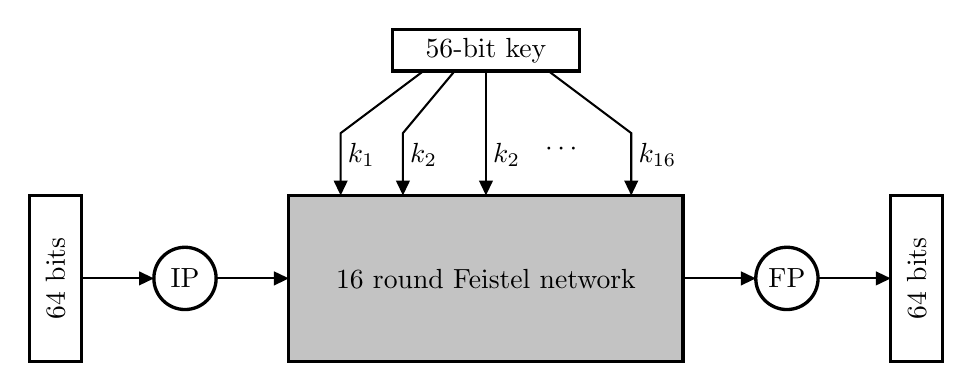
\begin{tikzpicture}[x=0.75pt,y=0.75pt,yscale=-1,xscale=1]
%uncomment if require: \path (0,169); %set diagram left start at 0, and has height of 169

%Shape: Rectangle [id:dp9082761089513578] 
\draw  [line width=1.2]  (0,80) -- (25,80) -- (25,160) -- (0,160) -- cycle ;
%Shape: Circle [id:dp03697940656912868] 
\draw  [line width=1.2]  (60,120) .. controls (60,111.72) and (66.72,105) .. (75,105) .. controls (83.28,105) and (90,111.72) .. (90,120) .. controls (90,128.28) and (83.28,135) .. (75,135) .. controls (66.72,135) and (60,128.28) .. (60,120) -- cycle ;
%Straight Lines [id:da7967662847402655] 
\draw    (25,120) -- (57,120) ;
\draw [shift={(60,120)}, rotate = 180] [fill={rgb, 255:red, 0; green, 0; blue, 0 }  ][line width=0.08]  [draw opacity=0] (7.14,-3.43) -- (0,0) -- (7.14,3.43) -- cycle    ;
%Straight Lines [id:da25423668245796893] 
\draw    (90,120) -- (122,120) ;
\draw [shift={(125,120)}, rotate = 180] [fill={rgb, 255:red, 0; green, 0; blue, 0 }  ][line width=0.08]  [draw opacity=0] (7.14,-3.43) -- (0,0) -- (7.14,3.43) -- cycle    ;
%Shape: Rectangle [id:dp8561305938166983] 
\draw  [fill={rgb, 255:red, 155; green, 155; blue, 155 }  ,fill opacity=0.6 ][line width=1.2]  (125,80) -- (315,80) -- (315,160) -- (125,160) -- cycle ;
%Shape: Circle [id:dp9835625221389512] 
\draw  [line width=1.2]  (350,120) .. controls (350,111.72) and (356.72,105) .. (365,105) .. controls (373.28,105) and (380,111.72) .. (380,120) .. controls (380,128.28) and (373.28,135) .. (365,135) .. controls (356.72,135) and (350,128.28) .. (350,120) -- cycle ;
%Straight Lines [id:da9164504674846901] 
\draw    (315,120) -- (347,120) ;
\draw [shift={(350,120)}, rotate = 180] [fill={rgb, 255:red, 0; green, 0; blue, 0 }  ][line width=0.08]  [draw opacity=0] (7.14,-3.43) -- (0,0) -- (7.14,3.43) -- cycle    ;
%Straight Lines [id:da18967570450355176] 
\draw    (380,120) -- (412,120) ;
\draw [shift={(415,120)}, rotate = 180] [fill={rgb, 255:red, 0; green, 0; blue, 0 }  ][line width=0.08]  [draw opacity=0] (7.14,-3.43) -- (0,0) -- (7.14,3.43) -- cycle    ;
%Shape: Rectangle [id:dp048056129270156456] 
\draw  [line width=1.2]  (415,80) -- (440,80) -- (440,160) -- (415,160) -- cycle ;
%Shape: Rectangle [id:dp764035049296157] 
\draw  [line width=1.2]  (175,0) -- (265,0) -- (265,20) -- (175,20) -- cycle ;
%Straight Lines [id:da0759384102778824] 
\draw    (190,20) -- (150,50) -- (150,77) ;
\draw [shift={(150,80)}, rotate = 270] [fill={rgb, 255:red, 0; green, 0; blue, 0 }  ][line width=0.08]  [draw opacity=0] (7.14,-3.43) -- (0,0) -- (7.14,3.43) -- cycle    ;
%Straight Lines [id:da5205997190861071] 
\draw    (205,20) -- (180,50) -- (180,77) ;
\draw [shift={(180,80)}, rotate = 270] [fill={rgb, 255:red, 0; green, 0; blue, 0 }  ][line width=0.08]  [draw opacity=0] (7.14,-3.43) -- (0,0) -- (7.14,3.43) -- cycle    ;
%Straight Lines [id:da9579629636144731] 
\draw    (220,20) -- (220,77) ;
\draw [shift={(220,80)}, rotate = 270] [fill={rgb, 255:red, 0; green, 0; blue, 0 }  ][line width=0.08]  [draw opacity=0] (7.14,-3.43) -- (0,0) -- (7.14,3.43) -- cycle    ;
%Straight Lines [id:da7033655636977068] 
\draw    (250,20) -- (290,50) -- (290,77) ;
\draw [shift={(290,80)}, rotate = 270] [fill={rgb, 255:red, 0; green, 0; blue, 0 }  ][line width=0.08]  [draw opacity=0] (7.14,-3.43) -- (0,0) -- (7.14,3.43) -- cycle    ;

% Text Node
\draw (12.5,120) node  [rotate=-270] [align=left] {$\displaystyle 64$ bits};
% Text Node
\draw (427.5,120) node  [rotate=-270] [align=left] {$\displaystyle 64$ bits};
% Text Node
\draw (220,120) node   [align=left] {$\displaystyle 16$ round Feistel network};
% Text Node
\draw (220,10) node   [align=left] {$\displaystyle 56$-bit key};
% Text Node
\draw (75,120) node   [align=left] {IP};
% Text Node
\draw (365,120) node   [align=left] {FP};
% Text Node
\draw (152,53.4) node [anchor=north west][inner sep=0.75pt]    {$k_{1}$};
% Text Node
\draw (182,53.4) node [anchor=north west][inner sep=0.75pt]    {$k_{2}$};
% Text Node
\draw (222,53.4) node [anchor=north west][inner sep=0.75pt]    {$k_{2}$};
% Text Node
\draw (292,53.4) node [anchor=north west][inner sep=0.75pt]    {$k_{16}$};
% Text Node
\draw (247,53.4) node [anchor=north west][inner sep=0.75pt]    {$\cdots $};


\end{tikzpicture}
  \caption{完整的DES电路}
  \label{fig:4-9}
\end{figure}

\begin{snote}[密钥扩展函数。]
DES 的密钥扩展函数 $G$ 将 $56$ 比特的密钥 $k$ 作为输入,输出 $16$ 个密钥 $k_1,\dots,k_{16}$,每个 $48$ 比特长。每个密钥 $k_i$ 都由从 $56$ 比特密钥 $k$ 中选出的 $48$ 个比特组成,每个 $k_i$ 都使用 $k$ 中比特的不同子集。
\end{snote}

\begin{snote}[DES 算法。]
完整的 DES 算法架构如图 \ref{fig:4-9} 所示,它包括对 DES 轮密码的 $16$ 次迭代,以及被称为 IP 和 FP 的初始和最后的置换。这些置换只是重新排列了 $64$ 比特的输入和输出,其中,FP 置换是 IP 置换的逆变换。

IP 和 FP 没有任何密码学意义,被包括在算法内的原因至今不明。由于比特置换在软件实现中很慢,但在硬件实现中却很快,一种理论认为,IP 和 FP 是为了故意减慢 DES 的软件实现才被加入的。
\end{snote}

\subsection{对 DES 的穷举搜索:DES 挑战}\label{subsec:4-2-2}

回顾一下,对分组密码 $(E,D)$ 的穷举搜索攻击(\ref{subsubsec:4-1-1-2} 小节)指的是这样的攻击:给予对手少量的明文分组 $x_1,\dots,x_Q\in\mathcal{X}$ 和使用 $\mathcal{K}$ 中的密钥 $k$ 加密它们得到的密文分组 $y_1,\dots,y_Q$。对手尝试所有可能的 $\mathpzc{k}\in\mathcal{K}$,直至找到一个密钥 $k$,能够将所有给定的明文分组映射到给定的密文分组上。如果给定的密文分组足够多,$k$ 就是唯一能够实现这种映射的密钥,而且它终将被对手发现。

对于像 DES 和 AES-128 这样的分组密码,仅需\emph{三}个分组就足以确保有唯一密钥能以较大概率将给定的明文分组映射到给定的密文分组。我们将在 \ref{subsec:4-7-2} 小节讨论理想密码及其特性时看到原因。现在我们只需知道,给定三个明文/密文分组对,攻击者就可以用穷举法找到秘钥 $k$。

在 1974 年设计 DES 时,对大小为 $2^{56}$ 的密钥空间进行穷举搜索攻击被认为是不可行的。但随着计算机硬件的持续发展,人们渐渐发现 $56$ 比特的密钥远远不够。

为了证明对 DES 的穷举搜索是可行的,RSA 数据安全部设置了一连串的挑战,称为 \textbf{DES 挑战}。规则很简单:在一个预先宣布的日期,RSA 数据安全部将会公布三个 DES 输入/输出对。第一个找到相应密钥的小组就能赢得一万美元。为了使挑战更具娱乐性,挑战包含 $n$ 个 DES 输出 $y_1,y_2,\dots,y_n$,其中的前三个输出 $y_1,y_2,y_3$ 是对下面这 $24$ 字节明文消息应用 DES 后得到的结果:
\begin{figure*}[h!]
  \centering
  

\tikzset{every picture/.style={line width=0.75pt}} %set default line width to 0.75pt        

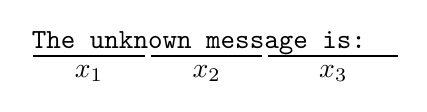
\begin{tikzpicture}[x=0.75pt,y=0.75pt,yscale=-1,xscale=1]
%uncomment if require: \path (0,40); %set diagram left start at 0, and has height of 40

%Straight Lines [id:da041820242795031604] 
\draw    (4,16) -- (58,16) ;
%Straight Lines [id:da47747795120640646] 
\draw    (61,16) -- (114.5,16) ;
%Straight Lines [id:da2450028819137724] 
\draw    (117.5,16) -- (180,16) ;

% Text Node
\draw (2,3) node [anchor=north west][inner sep=0.75pt]   [align=left] {
\texttt{The unknown message is:}
};
% Text Node
\draw (31,19.4) node [anchor=north] [inner sep=0.75pt]    {$x_{1}$};
% Text Node
\draw (87.75,19.4) node [anchor=north] [inner sep=0.75pt]    {$x_{2}$};
% Text Node
\draw (148.75,19.4) node [anchor=north] [inner sep=0.75pt]    {$x_{3}$};


\end{tikzpicture}
\end{figure*}

\noindent
该消息由 $3$ 个 DES 分组构成,每个分组为 $8$ 字节,也就是 $64$ 比特。目标是找到一个 DES 密钥,对于 $i=1,2,3$,该密钥能够将 $x_i$ 映射到 $y_i$。得到密钥后,挑战者就能够使用密钥来解密 $y_4,\dots,y_n$ 编码的秘密消息。

第一个挑战在 1997 年 1 月发布。\textsc{deschall} 项目组用 $96$ 天的时间解决了它。该团队在 $78,000$ 名志愿者的帮助下使用众包搜索的方式进行破解,这些志愿者贡献了他们自己设备的闲置算力。找到秘钥的志愿者获得了 $40\%$ 的奖金。解密后大家得知,$y_4,\dots,y_n$ 对应的明文是``强大的密码学使世界更加安全。" (Strong cryptography makes the world a safer place.)

第二个挑战于 1998 年 1 月发布。\textbf{distributed.net} 项目组使用了类似的但规模更大的众包搜索,仅用时 41 天就解决了该挑战。

1998 年初,电子前沿基金会 (Electronic Frontiers Foundation, EFF) 与 Paul Kocher 签订合同,建造一台专门的设备来进行针对 DES 的穷举密钥搜索。这台机器被称为\textbf{DeepCrack},耗资 25 万美元,包含大约 1900 个专用 DES 芯片,装在六个柜子里。这些芯片并行工作,每个芯片在指定的密钥空间中搜索。当 RSA 数据安全部在 1998 年 7 月发布下一个挑战时,DeepCrack 在 56 小时内就解决了这个挑战,并轻松赢得了一万美元的奖金。这还不足以支付机器的成本,但足以说明 DES 存在致命问题。

最后的挑战是在 1999 年 1 月发布的。在 DeepCrack 和 \emph{distributed.net} 的共同努力下,它在 22 小时内就被破解了。这在 DES 的棺材板上钉上了最后一颗钉子,表明 $56$ 比特的密钥可以在短短几个小时内就被破解。

在这个故事的末尾,2007 年,\textsc{copacobana} 团队建立了一个由现成的 120 块 FPGA 板组成的集群,总成本约为 1 万美元。该集群可以在大约 12.8 天内搜索完整个 $2^{56}$ 的 DES 密钥空间 \cite{guneysu2008cryptanalysis}。

上述所有工作将我们导向一个共同的结论,那就是 $56$ 比特密钥实在太短了。目前的最小安全密钥长度是 $128$ 比特。

\subsubsection{穷举搜索对 AES-128 是否奏效?}\label{subsubsec:4-2-2-1}

让我们把 DES 上的结论推广到 AES。虽然这些估计本身是不精确的,但它们在一定程度上说明了针对 AES 的穷举搜索的复杂性。AES 的密钥空间最小是 $2^{128}$。如果扫描一个 $2^{56}$ 的空间需要 22 小时,那么扫描一个 $2^{128}$ 大小的空间将需要:
\[
(22\;{\rm hours})\times2^{128-56}\approx1.18\times10^{20}\;{\rm years}
\]
即使计算速度和计算资源能提升十亿倍,即使 AES 计算比 DES 计算更快,所需的时间也远超人类的认知范围。因此,我们可以得出这样的结论:对 AES 进行暴力穷举式的搜索攻击是不现实的。然而,正如我们将在 \ref{sec:18-7} 节中讨论的,如果利用时空权衡这一经典思路,我们仍然可以对 AES-128 发起更复杂的暴力攻击。

\subsection{加强密码以抵抗穷举攻击:$3\mathcal{E}$构造}\label{subsec:4-2-3}

事实证明,DES 密码对复杂的攻击有很强的抵抗力。尽管经过了多年的分析,对 DES 最实用的攻击仍然是对整个密钥空间进行暴力穷举搜索。唯一的问题就是,$56$ 比特的密钥空间太小了。

一个自然而然的想法是,我们能否在不改变其内部结构的情况下加强密码的抗穷举攻击能力?最简单的解决方案是使用独立的密钥对密码进行多次迭代。

令 $\mathcal{E}=(E,D)$ 是一个定义在 $(\mathcal{K},\mathcal{X})$ 上的分组密码。我们定义分组密码 $3\mathcal{E}=(E_3,D_3)$ 为:
\[
E_3\big((k_1,k_2,k_3),\;x\big)
:=
E\big(k_3,\;E(k_2,\;E(k_1,x))\big)
\]
$3\mathcal{E}$ 密码的密钥在 $\mathcal{K}^3$ 上。基于 DES 算法的 $3\mathcal{E}$ 密码被称为 \textbf{Triple-DES},它的密钥长度为 $3\times56=168$ 比特。

\begin{snote}[安全性。]
为了分析 $3\mathcal{E}$ 密码的安全性,我们需要一个称为\emph{理想密码模型}的框架。我们将在本章末尾介绍这个框架,并在那一节中分析 $3\mathcal{E}$ 密码的安全性。
\end{snote}

\begin{snote}[Triple-DES 标准。]
NIST 批准 Triple-DES 在 2030 年前可以供政府使用。严格来说,NIST 版本的 Triple-DES 的定义为:
\[
E_3\big((k_1,k_2,k_3),\;x\big)
:=
E\big(k_3,\;D(k_2,\;E(k_1,x))\big)
\]
其原因是,如果设置 $k_1=k_2=k_3$,NIST 的 Triple-DES 就可以被还原为普通 DES,因此 Triple-DES 的硬件实现也可以直接复用于单一 DES 的场景中。这个修改不会影响我们对 Triple-DES 安全性的讨论。练习 \ref{exer:4-5} 中还讨论了 Triple-DES 的另一个变体。
\end{snote}

\subsubsection{$2\mathcal{E}$ 构造是不安全的}

虽然 Triple-DES 不容易被穷举搜索攻击所攻破,但它的性能比单一 DES 慢三倍,如表 \ref{tab:4-1} 所示。

那么为什么不使用 Double-DES 呢?它的密钥长度是 $2\times56=112$ 比特,这已经足以抵抗穷举搜索,而且它的性能也要比 Triple-DES 好得多。

问题在于,Double-DES 并不比单一 DES 更安全。更一般地说,令 $\mathcal{E}=(E,D)$ 是一个具有密钥空间 $\mathcal{K}$ 的分组密码。我们能够证明,定义为:
\[
E_2\big((k_1,k_2),\;x\big)
:=
E\big(k_2,\;E(k_1,x)\big)
\]
的 $2\mathcal{E}=(E_2,D_2)$ 构造不会比 $\mathcal{E}$ 更安全。针对它的攻击策略被称为\textbf{中间相遇 (meet in the middle)}。

假设我们得到了 $Q$ 个明文分组 $x_1,\dots,x_Q$,以及它们的 $2\mathcal{E}$ 加密 $y_i=E_2\big((k_1,k_2),x_i\big)$,其中 $i=1,\dots,Q$。我们下面展示如何在正比于 $|\mathcal{K}|$ 的时间内恢复密钥 $(k_1,k_2)$,即使密钥空间的大小为 $|\mathcal{K}|^2$。和单一 DES 的穷举搜索一样,我们只需少量的明文/密文对,就足以确保以高概率恢复唯一的密钥 $(k_1,k_2)$。事实上,对于像 Double-DES 这样的分组密码来说,$10$ 个分组就足以确保密钥的唯一性了。

\begin{theorem}\label{theo:4-2}
令 $\mathcal{E}=(E,D)$ 是一个定义在 $(\mathcal{K},\mathcal{X})$ 上的分组密码。存在一种算法 $\mathcal{A}_{{\rm E}X}$,它以 $Q$ 个明文/密文对 $(x_i,y_i)\in\mathcal{X}^2$作为输入,其中 $i=1,\dots,Q$,输出一个密钥对 $(\mathpzc{k}_1,\mathpzc{k}_2)\in\mathcal{K}^2$,满足:
\begin{equation}\label{eq:4-9}
y_i=E_2\big((\mathpzc{k}_1,\mathpzc{k}_2),\;x_i\big)
\quad\text{ for all }
i=1,\dots,Q
\end{equation}
其运行时间的主要成分是对算法 $E$ 和算法 $D$ 的总计 $2Q\cdot|\mathcal{K}|$ 次评估的耗时。
\end{theorem}

\begin{figure}
  \centering
  

\tikzset{every picture/.style={line width=0.75pt}} %set default line width to 0.75pt        

\begin{tikzpicture}[x=0.75pt,y=0.75pt,yscale=-1,xscale=1]
%uncomment if require: \path (0,230); %set diagram left start at 0, and has height of 230

%Shape: Rectangle [id:dp3572703895864946] 
\draw  [fill={rgb, 255:red, 255; green, 255; blue, 255 }  ,fill opacity=1 ][line width=1.5] [general shadow={fill=black,shadow xshift=2.25pt,shadow yshift=-2.25pt}] (90,0) -- (170,0) -- (170,80) -- (90,80) -- cycle ;
%Shape: Rectangle [id:dp5171740401100569] 
\draw  [fill={rgb, 255:red, 255; green, 255; blue, 255 }  ,fill opacity=1 ][line width=1.5] [general shadow={fill=black,shadow xshift=2.25pt,shadow yshift=-2.25pt}] (350,0) -- (430,0) -- (430,80) -- (350,80) -- cycle ;
%Straight Lines [id:da9329333357819998] 
\draw    (0,40) -- (87,40) ;
\draw [shift={(90,40)}, rotate = 180] [fill={rgb, 255:red, 0; green, 0; blue, 0 }  ][line width=0.08]  [draw opacity=0] (7.14,-3.43) -- (0,0) -- (7.14,3.43) -- cycle    ;
%Straight Lines [id:da7206318558961886] 
\draw    (170,40) -- (347,40) ;
\draw [shift={(350,40)}, rotate = 180] [fill={rgb, 255:red, 0; green, 0; blue, 0 }  ][line width=0.08]  [draw opacity=0] (7.14,-3.43) -- (0,0) -- (7.14,3.43) -- cycle    ;
%Straight Lines [id:da641366196961717] 
\draw    (430,40) -- (517,40) ;
\draw [shift={(520,40)}, rotate = 180] [fill={rgb, 255:red, 0; green, 0; blue, 0 }  ][line width=0.08]  [draw opacity=0] (7.14,-3.43) -- (0,0) -- (7.14,3.43) -- cycle    ;
%Shape: Circle [id:dp7654966486970967] 
\draw  [fill={rgb, 255:red, 0; green, 0; blue, 0 }  ,fill opacity=1 ] (256,40) .. controls (256,37.79) and (257.79,36) .. (260,36) .. controls (262.21,36) and (264,37.79) .. (264,40) .. controls (264,42.21) and (262.21,44) .. (260,44) .. controls (257.79,44) and (256,42.21) .. (256,40) -- cycle ;
%Straight Lines [id:da9777576592909831] 
\draw [line width=2.25]    (40,110) -- (235,110) ;
\draw [shift={(240,110)}, rotate = 180] [fill={rgb, 255:red, 0; green, 0; blue, 0 }  ][line width=0.08]  [draw opacity=0] (14.29,-6.86) -- (0,0) -- (14.29,6.86) -- cycle    ;
%Straight Lines [id:da8588229226837805] 
\draw [line width=2.25]    (285,110) -- (480,110) ;
\draw [shift={(280,110)}, rotate = 0] [fill={rgb, 255:red, 0; green, 0; blue, 0 }  ][line width=0.08]  [draw opacity=0] (14.29,-6.86) -- (0,0) -- (14.29,6.86) -- cycle    ;
%Shape: Rectangle [id:dp9192230055170565] 
\draw  [line width=1.5]  (210,130) -- (310,130) -- (310,220) -- (210,220) -- cycle ;
%Straight Lines [id:da33498550750905354] 
\draw    (210,150) -- (310,150) ;
%Straight Lines [id:da06955470431670019] 
\draw    (210,170) -- (310,170) ;
%Straight Lines [id:da1280441152779006] 
\draw    (210,190) -- (310,190) ;
%Straight Lines [id:da5216737251933607] 
\draw    (240,130) -- (240,220) ;

% Text Node
\draw (2,36.6) node [anchor=south west] [inner sep=0.75pt]    {$\bar{x}$};
% Text Node
\draw (517,36.6) node [anchor=south west] [inner sep=0.75pt]    {$\bar{y}$};
% Text Node
\draw (130,40) node    {$E(k_{1},\cdot)$};
% Text Node
\draw (390,40) node    {$E(k_{2},\cdot)$};
% Text Node
\draw (42,115) node [anchor=north west][inner sep=0.75pt]   [align=left] {步骤 $1$:};
% Text Node
\draw (382,115) node [anchor=north west][inner sep=0.75pt]   [align=left] {步骤 $2$:};
% Text Node
\draw (225,140) node    {$0$};
% Text Node
\draw (225,160) node    {$1$};
% Text Node
\draw (225,180) node    {$2$};
% Text Node
\draw (275,140) node    {$E(0,\bar{x})$};
% Text Node
\draw (275,160) node    {$E(1,\bar{x})$};
% Text Node
\draw (275,180) node    {$E(2,\bar{x})$};
% Text Node
\draw (225,205) node    {$\vdots$};
% Text Node
\draw (275,205) node    {$\vdots$};
% Text Node
\draw (42,143) node [anchor=west] [inner sep=0.75pt]   [align=left] {构建所有 $E(k_{1},\bar{x})$ 的表格};
% Text Node
\draw (382,135) node [anchor=north west][inner sep=0.75pt]   [align=left] {对每个 $\mathcal{K}$ 中的 $k$};
% Text Node
\draw (382,155) node [anchor=north west][inner sep=0.75pt]   [align=left] {在表中查找 $D(k_{2},\bar{y})$};


\end{tikzpicture}
  \caption{$2\mathcal{E}$上的中间相遇攻击}
  \label{fig:4-10}
\end{figure}

\begin{proof}
令 $\bar{x}:=(x_1,\dots,x_Q)$,$\bar{y}:=(y_1,\dots,y_Q)$。为了简化符号,我们用:
\[
\bar y=E_2\big((\mathpzc{k}_1,\mathpzc{k}_2),\;\bar x)=E(\mathpzc{k}_2,\;E(\mathpzc{k}_1,\bar x)\big)
\]
来描述式 \ref{eq:4-9} 中的 $Q$ 个映射。我们也可以把它写成:
\begin{equation}\label{eq:4-10}
D(\mathpzc{k}_2,\bar y)=E(\mathpzc{k}_1,\bar x)
\end{equation}
为了找到能满足式 \ref{eq:4-10} 的一对 $(\mathpzc{k}_1,\mathpzc{k}_2)$,算法 $\mathcal{A}_{{\rm E}X}$ 进行以下操作:

\vspace*{10pt}

\hspace*{5pt} 步骤 $1$:对于所有的 $\mathpzc{k}_1\in\mathcal{K}$,构建一张包含所有数对 $\big(\mathpzc{k}_1,\;E(\mathpzc{k}_1,\bar x)\big)$ 的表 $T$\\
\hspace*{26pt} 步骤 $2$:对于所有的 $\mathpzc{k}_2\in\mathcal{K}$,进行如下操作:\\
\hspace*{80pt} 计算 $\bar x\leftarrow D(\mathpzc{k}_2,\bar y)$\\
\hspace*{80pt} 查表:如果 $T$ 中包含数对 $(\cdot,\bar x)$,则\\
\hspace*{112pt} 令 $(\mathpzc{k}_1,\bar x)$ 为该数对,输出 $(\mathpzc{k}_1,\mathpzc{k}_2)$ 并停机

\vspace*{10pt}

\noindent
图 \ref{fig:4-10} 描述了这种中间相遇攻击。根据构造,算法输出的数对 $(\mathpzc{k}_1,\mathpzc{k}_2)$ 必然满足式 \ref{eq:4-10},正如定理所要求的那样。

算法 $\mathcal{A}_{{\rm E}X}$ 的步骤 $1$ 需要对 $E$ 进行 $Q\cdot|\mathcal{K}|$ 次评估,而步骤 $2$ 需要对 $D$ 进行 $Q\cdot|\mathcal{K}|$ 次评估。因此,该算法的全部运行时间大约是 $2Q\cdot|\mathcal{K}|$ 次对 $E$ 或 $D$ 进行评估的时间。我们假设向查找表 $T$ 中插入元素和查找元素的时间小于评估算法 $E$ 和 $D$ 的时间。
\end{proof}

如上所述,对于相对较小的 $Q$ 值,绝大多数情况下只有一个密钥对 $(\mathpzc{k}_1,\mathpzc{k}_2)$ 满足式 \ref{eq:4-9},它就会是定理 \ref{theo:4-2} 中算法 $\mathcal{A}_{{\rm E}X}$ 的输出。

定理 \ref{theo:4-2} 中算法 $\mathcal{A}_{{\rm E}X}$ 的运行时间与对 $\mathcal{E}$ 进行穷举搜索攻击的时间差不多,这表明 $2\mathcal{E}$ 并没有增强 $\mathcal{E}$ 对穷举搜索的抵抗力。然而,该定理只考虑了 $\mathcal{A}_{{\rm E}X}$ 的运行时间。需要注意的是,$\mathcal{A}_{{\rm E}X}$ 必须在内存中维护一张很大的查找表,这可能是很困难的。为了攻击 Double-DES,$\mathcal{A}_{{\rm E}X}$ 需要存储一张规模为 $2^{56}$ 的表,其中每个表项包含一个 DES 密钥和一条短的密文。总的来说,这相当于至少 $2^{60}$ 字节,也就是大约一百万 TB。虽然不是完全不可能,但获得如此多的存储可能是相当困难的。但是,攻击者可以通过时空权衡的方式来减少存储上的要求,方法是修改 $\mathcal{A}_{{\rm E}X}$,使其在运行过程中仅保留查找表的 ${1}/{\epsilon}$ 部分,代价是运行时间也要相应地增加一个 ${1}/{\epsilon}$ 因子。


\begin{snote}[Triple-DES 上的中间相遇攻击。]
类似的中间相遇攻击也适用于上一小节中的 $3\mathcal{E}$ 构造。虽然 $3\mathcal{E}$ 的密钥空间为 $\mathcal{K}^3$,但对 $3\mathcal{E}$ 的中间相遇攻击的时间大约为 $|\mathcal{K}|^2$,所需空间为 $|\mathcal{K}|$。在 Triple-DES 的情况下,该攻击需要对 DES 进行大约 $|\mathcal{K}|^2=2^{112}$ 次评估,这在实践中的运行时间实在太长了。因此,Triple-DES 可以抵御这种中间相遇攻击,这也是 Triple-DES 在实践中能够被广泛使用的原因。
\end{snote}

\subsection{案例研究:AES}\label{subsec:4-2-4}

虽然 Triple-DES 是 NIST 批准的密码,但它有一些明显的缺点。首先,Triple-DES 比 DES 慢三倍,在软件实现中表现很差。其次,$64$ 比特的分组长度对于一些重要的应用来说还是不够(即第\ref{chap:6}章中的应用)。到 20 世纪 90 年代中期,所有人都在期待一个新的联邦分组密码标准。

\begin{snote}[AES的历程。]
1997 年,NIST 发起了一个关于新的分组密码标准的提案征求,该标准被称为\textbf{高级加密标准 (Advanced Encryption Standard, AES)}。NIST 要求 AES 密码必须在 $128$ 比特分组上运行,并支持 $128$、$192$ 和 $256$ 比特三种密钥长度。截止到 1997 年 9 月,NIST 收到了 15 份提案,其中许多来自美国以外的国家。在举行了两次公开会议讨论这些提案后,NIST 在 1999 年将名单缩小到五个候选者。随后又进行了一轮激烈的密码分析,最终在 2000 年 4 月举行的 AES3 会议上,最后五个团队的代表分别作了发言,论证他们的标准为什么应该被选为 AES。2000 年 10 月,NIST 宣布一个来自比利时的分组密码 \textbf{Rijndael} 被选为 AES 密码。2001 年 11 月,当 AES 作为 NIST 的标准在 FIPS 197 中公布后,它正式成为了一个官方标准。这结束了长达五年的替换 DES 的标准化过程。

Rijndael 由比利时的密码学家 Joan Daemen 和 Vincent Rijmen 设计 \cite{daemen2002design}。AES 与原始版本的 Rijndael 密码略有不同。例如,Rijndael 支持大小为 $128$、$192$ 或 $256$ 比特的分组,而 AES 只支持 $128$ 比特的分组。
\end{snote}

\subsubsection{AES 算法}

和许多现实世界中的分组密码一样,AES 也是一个迭代密码,它将一个简单的轮密码迭代数次。迭代的次数取决于秘钥的长度:

\begin{center}
\begin{tabular}{c|c|c|c}
\begin{tabular}[c]{@{}c@{}}密码\\ 名称\end{tabular} &
  \begin{tabular}[c]{@{}c@{}}密钥长度\\  (比特)\end{tabular} &
  \begin{tabular}[c]{@{}c@{}}分组长度 \\ (比特)\end{tabular} &
  \begin{tabular}[c]{@{}c@{}}迭代\\ 轮数\end{tabular} \\ \hline\hline
AES-128 & 128 & 128 & 10 \\
AES-192 & 192 & 128 & 12 \\
AES-256 & 256 & 128 & 14 \\ \hline
\end{tabular}
\end{center}
例如,图 \ref{fig:4-11} 展示了一个包含十轮的 AES-128 密码的结构。这里的 $\Pi_{\rm AES}$ 是 $\{0,1\}^{128}$ 上的一个固定置换(一个双射),它不依赖于密钥。每轮的最后一步是将本轮密钥与 $\Pi_{\rm AES}$ 的输出进行异或。这样重复 $9$ 次,直至最后一轮使用一个稍加修改的置换 $\hat\Pi_{\rm AES}$。AES 的逆运算可以通过反向运行上面的步骤来完成。之所以只需要简单地反向就可以,是因为AES的每一步都是很容易反向运行的。

遵循图 \ref{fig:4-11} 所示结构的密码被称为\textbf{交替密钥密码 (alternating key cipher)} 或\textbf{迭代 Even-Mansour 密码 (iterated Even-Mansour cipher)}。如果每轮的置换 $\Pi_{\rm AES}$ 满足某些``理想"假设,这种密码就能够确保安全性。我们会在本章后面的定理 \ref{theo:4-14} 中详细分析这一点。

\begin{figure}
  \centering
  \tikzset{every picture/.style={line width=0.75pt}}

\begin{tikzpicture}[x=0.75pt,y=0.75pt,yscale=-1,xscale=1]

\draw  [->]  (50,195) -- (89,195) ;
\draw  [->]  (370,195) -- (409,195) ;
\draw  [->]  (510,195) -- (549,195) ;
\draw  [->]  (190,195) -- (269,195) ;
\draw  [->]  (240,60) -- (70,110) -- (70,188) ;
\draw  [->]  (265,60) -- (210,110) -- (210,188) ;
\draw  [->]  (279.5,60.75) -- (250,110) -- (250,188) ;
\draw  [->]  (320,60) -- (390,110) -- (390,188) ;
\draw  [->]  (360,60) -- (530,110) -- (530,188) ;

\draw  [fill={rgb, 255:red, 255; green, 255; blue, 255 }  ,fill opacity=1 ][line width=1.2]  (90,155) -- (190,155) -- (190,235) -- (90,235) -- cycle ;
\draw  [fill={rgb, 255:red, 255; green, 255; blue, 255 }  ,fill opacity=1 ][line width=1.2] [general shadow={fill=black,shadow xshift=2.25pt,shadow yshift=-2.25pt}] (0,180) -- (50,180) -- (50,210) -- (0,210) -- cycle ;
\draw  [fill={rgb, 255:red, 255; green, 255; blue, 255 }  ,fill opacity=1 ][line width=1.2]  (270,155) -- (370,155) -- (370,235) -- (270,235) -- cycle ;
\draw  [fill={rgb, 255:red, 255; green, 255; blue, 255 }  ,fill opacity=1 ][line width=1.2]  (410,155) -- (510,155) -- (510,235) -- (410,235) -- cycle ;
\draw  [fill={rgb, 255:red, 255; green, 255; blue, 255 }  ,fill opacity=1 ][line width=1.2] [general shadow={fill=black,shadow xshift=2.25pt,shadow yshift=-2.25pt}] (550,180) -- (600,180) -- (600,210) -- (550,210) -- cycle ;
\draw  [draw opacity=0][fill={rgb, 255:red, 255; green, 255; blue, 255 }  ,fill opacity=1 ] (220,190) -- (240,190) -- (240,200) -- (220,200) -- cycle ;
\draw  [line width=1.2]  (210,35) -- (390,35) -- (390,60) -- (210,60) -- cycle ;

\draw (25,195) node   [align=left] {输入};
\draw (70,194.98) node    {$\bigoplus $};
\draw (210,195) node    {$\bigoplus $};
\draw (390,194.98) node    {$\bigoplus $};
\draw (530,194.5) node    {$\bigoplus $};
\draw (250,195) node    {$\bigoplus $};
\draw (230,195) node    {$\cdots $};
\draw (575,195) node   [align=left] {输出};
\draw (112,178) node [anchor=north west][inner sep=0.75pt]  [font=\small] [align=left] {ByteSub};
\draw (112,193) node [anchor=north west][inner sep=0.75pt]  [font=\small] [align=left] {ShiftRow};
\draw (112,208) node [anchor=north west][inner sep=0.75pt]  [font=\small] [align=left] {MixColumns};
\draw (292,208) node [anchor=north west][inner sep=0.75pt]  [font=\small] [align=left] {MixColumns};
\draw (292,193) node [anchor=north west][inner sep=0.75pt]  [font=\small] [align=left] {ShiftRow};
\draw (292,178) node [anchor=north west][inner sep=0.75pt]  [font=\small] [align=left] {ByteSub};
\draw (412,158.4) node [anchor=north west][inner sep=0.75pt]  [font=\footnotesize]  {$\hat{\Pi }_{\mathrm{AES}} :$};
\draw (272,158.4) node [anchor=north west][inner sep=0.75pt]  [font=\footnotesize]  {$\Pi _{\mathrm{AES}} :$};
\draw (92,158.4) node [anchor=north west][inner sep=0.75pt]  [font=\footnotesize]  {$\Pi _{\mathrm{AES}} :$};
\draw (432,178) node [anchor=north west][inner sep=0.75pt]  [font=\small] [align=left] {ByteSub};
\draw (432,193) node [anchor=north west][inner sep=0.75pt]  [font=\small] [align=left] {ShiftRow};
\draw (140,247) node   [align=left][font=\small] {第 $1$ 轮};
\draw (320,247) node   [align=left][font=\small] {第 $9$ 轮};
\draw (460,247) node   [align=left][font=\small] {第 $10$ 轮};
\draw (300,47.5) node   [align=left] {$128$比特密钥};
\draw (72,113.4) node [anchor=north west][inner sep=0.75pt][font=\small]    {$k_{0}$};
\draw (212,113.4) node [anchor=north west][inner sep=0.75pt][font=\small]    {$k_{1}$};
\draw (252,113.4) node [anchor=north west][inner sep=0.75pt][font=\small]    {$k_{8}$};
\draw (392,113.4) node [anchor=north west][inner sep=0.75pt][font=\small]    {$k_{9}$};
\draw (532,113.4) node [anchor=north west][inner sep=0.75pt][font=\small]    {$k_{10}$};

\end{tikzpicture}
  \caption{AES-128分组密码的示意图}
  \label{fig:4-11}
\end{figure}

\begin{snote}[AES 轮置换。]
置换 $\Pi_{\rm AES}$ 是由集合 $\{0,1\}^{128}$ 上的三个可逆操作序列组成的。输入的 $128$ 比特会被组织成一个 $4\times4$ 的元胞数组,其中每个元胞是 $8$ 比特。然后,以下三个可逆运算会在这个 $4\times4$ 的数组上依次执行:
\begin{enumerate}
	\item $\mathtt{SubBytes}$:令 $S:\{0,1\}^8\to\{0,1\}^8$ 是一个固定置换(一个双射)。这个置换会被应用于所有 $16$ 个元胞上,一次一个元胞。在 AES 标准中,$S$ 被设计成一个包含 $256$ 个表项的硬编码表。在数学上,$S$ 没有不动点,即对于任意的 $x\in\{0,1\}^8$,$S(x)\neq x$ 都成立。$S$ 也没有逆不动点,即对于任意的 $x\in\{0,1\}^8$,$S(x)\neq \bar x$ 也都成立,其中 $\bar x$ 表示 $x$ 的按位补码。这些要求是抵御 \ref{subsec:4-3-1} 小节中将要讨论的某些攻击所必须的。
	\item $\mathtt{ShiftRows}$:这一步对输入的 $4\times4$ 数组的四行进行按行循环移位:第一行不变,第二行向左循环移动 $1$ 字节,第三行向左循环移动 $2$ 字节,第四行向左循环移动 $3$ 字节。更直观地说,这一步进行了下面这样的转换:
	\begin{equation}\label{eq:4-11}
    \begin{pmatrix}
       a_0 & a_1 & a_2 & a_3\\
       a_4 & a_5 & a_6 & a_7\\
       a_8 & a_9 & a_{10} & a_{11}\\
       a_{12} & a_{13} & a_{14} & a_{15}
    \end{pmatrix}
    \Longrightarrow
    \begin{pmatrix}
       a_0 & a_1 & a_2 & a_3\\
       a_5 & a_6 & a_7 & a_4\\
       a_{10} & a_{11} & a_{8} & a_{9}\\
       a_{15} & a_{12} & a_{13} & a_{14}
    \end{pmatrix}
    \end{equation}
    \item $\mathtt{MixColumns}$:在这一步中,$4\times4$ 数组被视为一个矩阵,该矩阵会与一个固定的矩阵相乘,其中的算术是有限域 ${\rm GF}(2^8)$ 上的运算。有限域 ${\rm GF}(2^8)$ 中的元素可以表示成 ${\rm GF}(2)$ 中元素的不大于 $8$ 阶的多项式,其中的乘法以既约多项式 $x^8+x^4+x^3+x+1$ 为模。具体来说,$\mathtt{MixColumns}$ 的变换是这样的:
    \begin{equation}\label{eq:4-12}
    	\begin{pmatrix}	
    		02 & 03 & 01 & 01\\
    		01 & 02 & 03 & 01\\
    		01 & 01 & 02 & 03\\
    		03 & 01 & 01 & 02
    	\end{pmatrix}
    	\times
    	\begin{pmatrix}
    		a_0 & a_1 & a_2 & a_3\\
    		a_5 & a_6 & a_7 & a_4\\
    		a_{10} & a_{11} & a_{8} & a_{9}\\
    		a_{15} & a_{12} & a_{13} & a_{14}
    	\end{pmatrix}
    	\Longrightarrow
    	\begin{pmatrix}
    		a_0' & a_1' & a_2' & a_3'\\
    		a_4' & a_5' & a_6' & a_7'\\
    		a_8' & a_9' & a_{10}' & a_{11}'\\
    		a_{12}' & a_{13}' & a_{14}' & a_{15}'
    	\end{pmatrix}
    \end{equation}
    这里,标量 $01,02,03$ 被解释为 ${\rm GF}(2^8)$ 上的元素,并用它们的二进制表示(比如说,$03$ 代表 ${\rm GF}(2^8)$ 上的元素 $x+1$)。这个固定矩阵在 ${\rm GF}(2^8)$ 上是可逆的,所以整个变换也是可逆的。
\end{enumerate}

图 \ref{fig:4-11} 所示的 AES 电路中使用的置换 $\Pi_{\rm AES}$ 就由 $\mathtt{SubBytes}$、$\mathtt{ShiftRows}$ 和 $\mathtt{MixColumns}$ 这三个置换按顺序排列而成。在最后一轮,AES 会使用一个稍微不同的函数,我们称之为 $\hat\Pi_{\rm AES}$。这个函数大体上与 $\Pi_{\rm AES}$ 相同,只是省略了 $\mathtt{MixColumns}$ 这一步骤,这是为了使 AES 的解密电路看起来与 AES 的加密电路类似。\cite{dunkelman2010effects} 讨论了这种省略带来的安全影响。

因为 $\Pi_{\rm AES}$ 的每一步都是容易逆运算的,所以整个 $\Pi_{\rm AES}$ 置换的全过程也容易逆运算,这也是解密所需要的。
\end{snote}

\begin{snote}[使用预计算表实现 AES。]
AES 的轮函数是由我们之前介绍的置换 $\Pi_{\rm AES}$ 构建的,它包含 $\mathtt{SubBytes}$、$\mathtt{ShiftRows}$ 和 $\mathtt{MixColumns}$ 这三个步骤。但是 AES 的设计者并不是按照这种方式实现 $\Pi_{\rm AES}$ 的,他们提出了一种更高效的方式,能够利用四个固定的查找表 $T_0,T_1,T_2,T_3$ 一次性地完成上面的三个步骤。

为了解释其工作原理,回顾一下,$\Pi_{\rm AES}$ 将一个 $4\times4$ 的矩阵 $A=(a_i)_{i=0,\dots,15}$ 作为输入,并输出一个尺寸相同的矩阵 $A'=\Pi_{\rm AES}(A)$。令 $S[a]$ 为对输入的 $a\in\{0,1\}^8$ 进行 $\mathtt{SubBytes}$ 运算后的结果。类似地,回顾一下,$\mathtt{MixColumns}$ 将当前状态乘以一个固定的 $4\times4$ 矩阵 $M$。令 $M[i]$ 表示 $M$ 的第 $i$ 列,$A'[i]$ 表示 $A'$ 的第 $i$ 列。

现在看一下式 \ref{eq:4-12},我们可以把 $\Pi_{\rm AES}(A)$ 输出的四列表示为:
\begin{equation}\label{eq:4-13}
	\begin{aligned}
		A'[0] & = M[0]\cdot S[a_0]+M[1]\cdot S[a_5]+M[2]\cdot S[a_{10}]+M[3]\cdot S[a_{15}]\\ 
		A'[1] & = M[0]\cdot S[a_1]+M[1]\cdot S[a_6]+M[2]\cdot S[a_{11}]+M[3]\cdot S[a_{12}]\\ 
		A'[2] & = M[0]\cdot S[a_2]+M[1]\cdot S[a_7]+M[2]\cdot S[a_8]+M[3]\cdot S[a_{13}] \\ 
		A'[3] & = M[0]\cdot S[a_3]+M[1]\cdot S[a_4]+M[2]\cdot S[a_9]+M[3]\cdot S[a_{14}]
	\end{aligned}
\end{equation}
其中的加法和乘法都是在域 ${\rm GF}(2^8)$ 上进行的。对于 $i=0,1,2,3$,每一列 $M[i]$ 都是 ${\rm GF}(2^8)$ 上的一个 $4$ 字节向量,而 $S[a_i]$ 是 ${\rm GF}(2^8)$ 上的 $1$ 字节标量。

式 \ref{eq:4-13} 中的每一项都可以用一张固定的预计算表来快速评估。对于 $i=0,1,2,3$,我们定义一张有 $256$ 项的表 $T_i$ 如下:
\[
\text{对于}\;a\in\{0,1\}^8:\quad\quad
T_i[a]:=M[i]\cdot S[a]\quad\in\{0,1\}^{32}
\]
将这些表格接驳到式 \ref{eq:4-13} 上,我们就可以得到一个快速计算 $\Pi_{\rm AES}(A)$ 的方法:
\[
\begin{aligned}
A'[0] & = T_0[a_0]+T_1[a_5]+T_2[a_{10}]+T_3[a_{15}]\\
A'[1] & = T_0[a_1]+T_1[a_6]+T_2[a_{11}]+T_3[a_{12}]\\
A'[2] & = T_0[a_2]+T_1[a_7]+T_2[a_8]+T_3[a_{13}]\\
A'[3] & = T_0[a_3]+T_1[a_4]+T_2[a_9]+T_3[a_{14}]
\end{aligned}
\]
以这种方式实现的 AES 电路就是一个简单的查表序列。由于每张 $T_i$ 表中包含 $256$ 个表项,每个表项大小为 $4$ 字节,所以四张表的总大小也不过 4 KB。$M$ 矩阵的循环结构使我们可以进一步将四张表压缩到 2 KB,而不对性能产生大的影响。

式 \ref{eq:4-13} 的一个例外是 AES 的最后一轮,这一轮中的 $\mathtt{MixColumns}$ 步骤被省略了。为了计算最后一轮,我们需要第五张 $256$ 字节的表 $S$,它只包含 $\mathtt{SubBytes}$ 的操作。

这个 AES 优化并不是必须的。如果环境极度受限以至于没有足够的空间存储 4 KB 的查找表,你也可以直接按照基本原理用代码分别实现 $\Pi_{\rm AES}$ 的三个步骤,这节约了存储空间,但运算速度可能会慢一点。因此,AES 可以同时适用于有算力约束和算力不受限的环境。

必须要注意的是,这种查表优化的 AES 实现很可能会受到缓存定时攻击,我们将在 \ref{subsec:4-3-2} 小节中介绍这种攻击。
\end{snote}


\begin{snote}[AES-128 的密钥扩展方法。]
回顾图 \ref{fig:4-11},我们看到 AES-128 的密钥扩展算法需要生成 $11$ 个轮密钥 $k_0,\dots,k_{10}$,其中的每个轮密钥都是 $128$ 比特。为此,$128$ 比特的 AES 密钥会被分割成四个 $32$ 比特长的字 $w_{0,0},w_{0,1},w_{0,2},w_{0,3}$,这些字构成了第一个轮密钥 $k_0$。其余 $10$ 个轮回密钥按以下顺序产生:对于 $i=1,\dots,10$,$128$比特的轮密钥 $k_i=(w_{i,0},w_{i,1},w_{i,2},w_{i,3})$ 由上一个轮密钥 $k_{i-1}=(w_{i-1,0},w_{i-1,1},w_{i-1,2},w_{i-1,3})$ 产生,方式如下:
 
\vspace*{10pt}

\hspace*{5pt} $w_{i,0}\leftarrow w_{i-1,0}\oplus g_i(w_{i-1,3})$\\
\hspace*{26pt} $w_{i,1}\leftarrow w_{i-1,1}\oplus w_{i,0}$\\
\hspace*{26pt} $w_{i,2}\leftarrow w_{i-1,2}\oplus w_{i,1}$\\
\hspace*{26pt} $w_{i,3}\leftarrow w_{i-1,3}\oplus w_{i,2}$

\vspace*{10pt}

\noindent
这里的函数 $g_i:\{0,1\}^{32}\to\{0,1\}^{32}$ 是 AES 标准中规定的一个固定函数。它对 $4$ 字节输入进行以下三步操作:
(1) 对 $4$ 字节输入进行 $1$ 字节循环左移,
(2) 对得到的 $4$ 字节中的每个字节分别计算 $\mathtt{SubBytes}$,然后
(3) 将最左边的字节与一个固定的轮常数 $c_i$ 进行异或。
轮常数 $c_1,\dots,c_{10}$ 也是在 AES 标准中规定的,其中 $c_i$ 就是 ${\rm GF}(2^8)$ 上的元素 $x^{i-1}$,它被当作一个 $8$ 比特序列处理。

AES-192 和 AES-256 的密钥扩展方法与 AES-128 的类似。对于 AES-192 来说,每次迭代都会产生 $6$ 个 $32$ 比特的字(共计 $192$ 比特),但只有前 $4$ 个字(共计 $128$ 比特)会被用作 AES 的轮密钥。对于 AES-256,每次迭代产生 $8$ 个 $32$ 比特的字(共计 $256$ 比特),也只有前 $4$ 个字(共计 $128$ 比特)会被用作 AES 的轮密钥。

AES 的密钥扩展方法被有意设计成是可逆的:只要给定最后一轮的密钥,我们就可以反过来恢复完整的 AES 秘钥 $k$。这样做的原因是为了确保每个 AES-128 的轮密钥,就其本身而言,具有与 AES-128 的秘钥 $k$ 相同的熵。不幸的是,可逆性也有助于攻击,它可以被用来发起对 AES 的相关密钥攻击和边信道攻击,我们将在之后讨论这些攻击。
\end{snote}

\begin{snote}[AES的安全性。]
AES 算法经受住了针对它的各种复杂的密码分析尝试。截止到成稿时,最有名的攻击有如下这些:
\begin{itemize}
	\item \textbf{密钥恢复}。密钥恢复攻击是指对手在得到若干明文/密文对的情况下,使用如穷举搜索攻击等方式从这些明密文对中恢复密钥的攻击方式。已知最好的对 AES-128 的密钥恢复攻击需要进行 $2^{126.1}$ 次 AES 计算 \cite{bogdanov2011biclique}。这比穷举搜索要快四倍左右,但需要的时间仍然太长了。因此这种攻击对 AES-128 的安全性威胁不大。
	
	对 AES-192 最好的攻击需要进行 $2^{189.74}$ 次 AES 计算,这也只比穷举搜索快了四倍左右。对 AES-256 的最著名的攻击需要 $2^{254.42}$ 次 AES 计算,这比穷举搜索快三倍。这些攻击都不能影响任何一个 AES 变体的安全性。
	\item \textbf{相关密钥攻击(related key attack)}。在 $\ell$ 路相关密钥攻击中,对手得到了 $\ell$ 张明文/密文对的列表:对于 $i=1,\dots,\ell$,第 $i$ 张表是用密钥 $k_i$ 生成的。重点是,所有 $\ell$ 个密钥 $k_1,\dots,k_\ell$ 都必须满足对手选择的一些固定关系。攻击者的目标是恢复其中一个密钥,比如说 $k_1$。在实现良好的密码系统中,密钥总是独立随机生成的,因此不太可能满足攻击者所需的关系。因此,相关密钥攻击通常不会威胁到正确的加密实现。

    AES-256 容易受到相关密钥攻击,该攻击利用了其相对简单的密钥扩展机制 \cite{biryukov2009related}。该攻击需要四个相关密钥 $k_1,k_2,k_3,k_4$,其中的关系是一个简单的异或关系:它要求 $k_1\oplus k_2$,$k_1\oplus k_3$ 和 $k_2\oplus k_4$ 的某些比特被置为特定值。然后给定由这四个密钥产生的明密文对的列表,攻击者可以在 $2^{99.5}$ 时间内恢复这四个密钥。这比在 AES-256 上进行穷举搜索的时间要快得多。虽然这种攻击相当有趣,但它并不能影响 AES-256 在完善的系统中的安全性。
\end{itemize}
\end{snote}

\begin{snote}[AES的硬件实现。]
在 AES 刚被标准化为美国国家加密标准的时候,大多数的实现都还是基于软件的。软件产品对 AES 的广泛采用,促使所有主要的处理器供应商扩展他们的指令集,以增加对 AES 硬件实现的支持。

例如,英特尔在其 Xeon 和 Core 系列处理器中增加了名为 \textbf{AES-NI} 的新指令,以加快在软件中使用 AES 的过程。新指令的工作原理如下:
\begin{itemize}
	\item $\tt{AESKEYGENASSIST}$:运行密钥扩展程序,从 AES 密钥中生成 AES 轮密钥。
	\item $\tt{AESENC}$:运行一轮 AES 轮加密算法。该指令的调用方法是:
	\[
    \tt{AESENC\;\;xmm15,\;\;xmm1}
    \]
    其中 $\tt xmm15$ 寄存器保存 $128$ 比特数据分组,$\tt xmm1$ 寄存器保存该轮的 $128$ 比特轮密钥。得到的 $128$ 比特分组会被写入寄存器 $\tt xmm15$。在 AES 的前九轮中,可以事先将轮密钥加载到寄存器 $\tt{xmm1,\dots,xmm9}$ 中,然后调用九次该指令。
    \item $\tt AESENCLAST$:调用与 $\tt AESENC$ 类似的指令来运行 AES 算法的最后一轮。回顾一下,AES 最后一轮的功能与前面几轮稍有不同,它省略了 $\tt MixColumns$ 这一步。
    \item $\tt AESDEC$ 和 $\tt AESDECLAST$:运行 AES 解密算法,与加密指令类似。
\end{itemize}
这些 AES-NI 硬件指令的速度比极尽所能去优化 AES 的软件实现还要更快。Emilia Käsper 在 2009 年的实验表明,在英特尔 Core 2 处理器上,使用 AES-NI 指令的 AES 需要 $1.35$ 周期/字节(流水线化),而优化的软件实现则需要 $7.59$ 周期/字节。

在英特尔 2015 年推出的 Skylake 处理器中,$\tt AESENC$、$\tt AESDEC$ 和 $\tt AESENCLAST$ 指令各需要四个周期来完成。这些指令是完全流水线式的,因此每个周期都可以发射一条新指令。换句话说,英特尔将 $\tt AESENC$ 的执行划分为四个阶段的流水线,四个 AES 分组可以由流水线的不同阶段同时处理。虽然处理一个 AES-128 分组需要(4 个周期)$\times$(10 轮)$=$($40$ 个周期)($2.5$ 周期/字节),但在一条流水线上处理四个分组只需要 $44$ 个周期($0.69$ 周期/字节)。因此,流水线可以将 AES 的速度提高近 $4$ 倍。正如我们将在下一章看到的,这在选择我们用来加密长消息的确切方法时起到了重要的作用:选择一种能尽可能地利用并行性来保持流水线繁忙的加密方法是最理想的。

除了速度之外,AES 的硬件实现还提供了更好的安全性,因为它可以抵御下一节中将介绍的边信道攻击。
\end{snote}
\section{针对分组密码的复杂攻击}

像 AES 这样被广泛使用的分组密码在被标准化之前都要经过一个漫长的选择过程,并在之后持续受到密码分析的影响。在本节中,我们将调查多年来开发的一些攻击技术。

在 \ref{subsec:4-3-1} 小节,我们将讨论对密码设计的攻击,这些攻击可能会从对明文/密文对的观察中获得关于密钥的信息。与暴力穷举搜索攻击不同,这些\textbf{算法攻击(algorithmic attack)}依赖于对特定分组密码内部结构的巧妙分析。

在 \ref{subsec:4-3-2} 小节,我们将介绍一种非常不同的攻击类别,称为\textbf{边信道攻击(side-channel attack)}。在分析任何密码系统时,我们都会考虑对手与密码系统的用户交互的情况。在这些交互的过程中,对手收集到的信息可能会帮助其破解系统。在本书中,我们通常假设这种信息仅限于用户的输入/输出行为(例如明文/密文对)。然而,这个假设忽略了一个事实,即\textbf{计算本身是一个物理过程}。正如我们将看到的,在某些情况下,对手有可能通过测量计算的物理特性,例如运行时间或功耗,来破解一个密码系统。

另一类对密码系统的物理实现的攻击是\textbf{错误注入攻击(fault-injection attack)},我们将在 \ref{subsec:4-3-3} 小节讨论。最后,在 \ref{subsec:4-3-4} 小节,我们还会考虑另一类算法攻击,即对手可以利用\textbf{量子力学}定律来加快其计算速度。

这些巧妙的攻击导出了两个非常重要的观点:
\begin{enumerate}
	\item 密码学的普通用户应该只使用像 AES 这样的标准化算法,而不是去设计他们自己的分组密码。
	\item 最好不要自己实现算法,因为自己的实现很可能容易受到边信道攻击。最好是使用已经被广泛验证的成熟密码库。
\end{enumerate}
为了进一步强调这些观点,我们鼓励任何第一次了解 AES 内部工作原理的人作出以下娱乐性的承诺,它最早由杰夫·莫瑟(Jeff Moser)提出:
\begin{quote}
我保证,一旦我看到AES到底有多简单,我就不会在生产代码中去实现它,就算它真的很有趣。这个承诺将一直有效,直到我了解了所有关于边信道攻击及其反制对策的知识,以至于我对自己实现AES失去兴趣。
\end{quote}

\subsection{算法攻击}\label{subsec:4-3-1}

攻击分组密码的设计是一个庞大的领域,其中包含许多复杂的技术:线性密码分析、差分密码分析、滑动攻击、飞去来器攻击等等。在此,我们简要介绍一种称为\emph{线性密码分析}的技术,该技术已被成功用于破解 DES 密码。这种技术是由日本密码学家松井充(Matsui Mitsuru)提出的,它解释了这个问题,即为什么我们一直说设计有效的密码是非常具有挑战性的一项工作。另外,这种方法已经被证明对 AES 不起作用。

\begin{snote}[线性密码分析。]
令 $(E,D)$ 是一个数据分组和密钥都是比特序列的分组密码,即 $\mathcal{M}=\mathcal{C}=\{0,1\}^n$,$\mathcal{K}=\{0,1\}^h$。

对于一个比特序列 $m\in\{0,1\}^n$ 和一组比特位置 $S\subseteq\{0,\dots,n-1\}$,我们用 $m[S]$ 表示 $S$ 中对应位置的比特的异或。也就是说,如果 $S=\{i_1,\dots,i_\ell\}$,则 $m[S]:=m[i_1]\oplus\dots\oplus m[i_\ell]$。

如果存在比特位置集合 $S_0,S_1\subseteq\{0,\dots,n-1\}$ 和 $S_2\subseteq\{0,\dots,h-1\}$ 使得对于\emph{所有的}密钥 $k\in\mathcal{K}$ 和\emph{随机挑选的} $m\in\mathcal{M}$,都有:
\begin{equation}\label{eq:4-14}
\Pr[m[S_0]\oplus E(k,m)[S_1]=k[S_2]]\geq\frac{1}{2}+\epsilon
\end{equation}
我们就称分组密码 $(E,D)$ 具有\textbf{线性关系 (linear relation)}。其中的 $\epsilon$ 是一个不可忽略不计的值,称为\textbf{偏差 (bias)}。对于一个``理想的"密码,明文和密文表现地就像两个相互独立的序列一样,因此式 \ref{eq:4-14} 中的关系 $m[S_0]\oplus E(k,m)[S_1]=k[S_2]$ 恰好以 $1/2$ 的概率成立,因此有 $\epsilon=0$。令人惊讶的是,DES 密码就有一个线性关系,其偏差 $\epsilon$ 虽小但不可忽略不计。

让我们看看线性关系是如何导致攻击的。考虑一个密码 $(E,D)$,它有一个如式 \ref{eq:4-14} 那样的线性关系,对于某个不可忽略不计的 $\epsilon>0$ 成立。我们假设线性关系是明确的,所以攻击者知道关系中使用的集合 $S_0$,$S_1$ 和 $S_2$。假设对于某个未知的密钥 $k\in\mathcal{K}$,攻击者能够获得许多明文/密文对 $(m_i,c_i)$,$i=1,\dots,t$。我们假设消息 $m_1,\dots,m_t$ 是从 $\mathcal{M}$ 中独立均匀采样的,并且 $c_i=E(k,m_i)$ 对于 $i=1,\dots,t$ 成立。利用这些信息,假设攻击者得到了足够多的明文/密文对,它就可以了解关于密钥 $k$ 的一个比特的信息,即 $k[S_2]\in\{0,1\}$。下面的定理说明了这一点。
\end{snote}

\begin{lemma}\label{lemma:4-3}
假设 $(E, D)$ 是一个满足式 \ref{eq:4-14} 的分组密码。令 $m_1,\dots,m_t$ 是从消息空间 $\mathcal{M}$ 中均匀独立采样得到的消息,令 $c_i:=E(k,m_i)$ 对 $i=1,\dots,t$ 成立。那么:
\begin{equation}\label{eq:4-15}
\Pr
\Bigm[
k[S_2]={\rm Majority}^t_{i=1}(m_i[S_0]\oplus c_i[S_1])
\Bigm]
\geq1-e^{-{t\epsilon^2}/{2}}
\end{equation}
\end{lemma}


这里,$\rm Majority$ 表示对给定的比特进行多数投票;例如,对于输入 $(0,0,1)$,$\rm Majority$ 的结果就是 $0$;对于 $(0,1,1)$,结果就是 $1$。直接应用经典切尔诺夫约束(Chernoff bound)就可以证明该引理。

式 \ref{eq:4-15} 中的下界表明,一旦给定的明文/密文对的数量超过 ${4}/{\epsilon^2}$,$\rm Majority$ 的输出等于 $k[S_2]$ 的概率就会超过 $86\%$。这样,攻击者就可以从给定的明文/密文对中计算出 $k[S_2]$,并获得关于密钥的一个比特的信息。虽然仅一比特的信息看起来可能不多,但它是迈向更强攻击的垫脚石,而后者可能就能暴露整个密钥。

\begin{snote}[对 DES 的线性密码分析。]
松井充表明,DES 密码中的 $14$ 轮加密中存在一个线性关系,其中的偏差至少有 $\epsilon\geq2^{-21}$。事实上,我们可以得到两个线性关系:其中一个利用 DES 加密电路的线性性质,另一个则利用解密电路的线性性质。对于一个 $64$ 比特的明文 $m$,令 $m_{\rm L}$ 和 $m_{\rm R}$ 分别表示 $m$ 的左 $32$ 比特和右 $32$ 比特。同样地,对于一个 $64$ 比特的密文 $c$,令 $c_{\rm L}$ 和 $c_{\rm R}$ 分别表示 $c$ 的左 $32$ 比特和右 $32$ 比特。那么 DES 的中包含的两个线性关系是:
\begin{equation}\label{eq:4-16}
	\begin{aligned}
		m_{\rm R}[17,18,24]\oplus c_{\rm L}[7,18,24,29]\oplus c_{\rm R}[15] & = k[S_{\rm e}]\\
		c_{\rm R}[17,18,24]\oplus m_{\rm L}[7,18,24,29]\oplus m_{\rm R}[15] & = k[S_{\rm d}]
	\end{aligned}
\end{equation}
其中 $S_{\rm e}$ 和 $S_{\rm d}$ 是 $56$ 比特密钥 $k$ 的某两个比特位置。当应用到 $14$ 轮 DES 中时,上面两个关系的偏差都是 $\epsilon\geq2^{-21}$。

通过将 DES 的首轮和末轮(即第$1$轮和第$16$轮)纳入这它们,这两个关系就可以被扩展到全部 $16$ 轮 DES 中。令 $k_1$ 是第一轮密钥,$k_{16}$ 是最后一轮密钥。根据 DES 轮函数的定义,我们从式 \ref{eq:4-16} 可以得到全部 $16$ 轮 DES 电路的以下关系:
\begin{align}
	\Big(m_{\rm L}\oplus F(k_1,m_{\rm R})\Big)[17,18,24]\oplus c_{\rm R}[7,18,24,29]\oplus\Big(c_{\rm L}\oplus F(k_{16},c_{\rm R})\Big)[15]=k[S_{\rm e}'] \label{eq:4-17}\\
	\Big(c_{\rm L}\oplus F(k_{16},c_{\rm R})\Big)[17,18,24]\oplus m_{\rm R}[7,18,24,29]\oplus\Big(m_{\rm L}\oplus F(k_1,m_{\rm R})\Big)[15]=k[S_{\rm d}'] \label{eq:4-18}
\end{align}
其中 $S_{\rm e}'$ 和 $S_{\rm d}'$ 是 $56$ 比特密钥 $k$ 中某两个比特的位置,即$S_{\rm e}', S_{\rm d}'\in\{0,\dots,55\}$。

我们首先考察式 \ref{eq:4-17} 中的关系。$F(k_1,m_{\rm R})$ 的第 $17,18,24$ 比特是同一个的 S 盒的结果,因此它们只取决于 $k_1$ 的 $6$ 个比特。类似地,$F(k_{16},c_{\rm R})[15]$ 只取决于 $k_{16}$ 的 $6$ 个比特。因此,式 \ref{eq:4-17} 的左手边只取决于密钥 $k$ 的 $12$ 比特,我们用 $k^{(12)}$ 表示这 $12$ 个比特。我们知道,当这 $12$ 比特被设定为正确的值时,式 \ref{eq:4-17} 的左手边在计算随机的明文/密文对时相对于 $k[S_{\rm e}']$ 表现出约 $2^{-21}$ 的偏差。而当这 $12$ 比特被设定为错误的值时,式 \ref{eq:4-17} 中的偏差就小得多。正如我们将要看到的,这个结论已经在实验中得到了验证。

这一观察让攻击者能以下面介绍的方式恢复密钥 $k$ 的 $12$ 比特 $k^{(12)}$。给定一个由 $t$ 个明文/密文对组成的列表 $L$(例如 $t=2^{43}$),攻击者进行以下操作:
\begin{itemize}
    \item 步骤 $1$:对于密钥比特 $k^{(12)}$ 的 $2^{12}$ 的候选情况中的每一个,计算式 \ref{eq:4-17} 中的偏差。也就是说,对 $L$ 中的所有 $t$ 个明文/密文对计算式 \ref{eq:4-17} 的左手边,令 $t_0$ 为表达式结果为 $0$ 的次数。偏差的计算方法是$\epsilon=|(t_0/t)-(1/2)|$。这就产生了一个由 $2^{12}$ 个偏差组成的向量,每一个 $k^{(12)}$ 的 $12$ 比特候选值都对应着一个偏差。
	\item 步骤 $2$:将 $2^{12}$ 个候选值按其偏差从大到小排序。如果给定的明文/密文对的列表 $L$ 足够大,那么偏差最高的 $12$ 位候选值就最有可能等于 $k^{(12)}$,这样就可以恢复密钥中的 $12$ 比特。一旦知道了 $k^{(12)}$,我们就可以用引理 \ref{lemma:4-3} 确定 $k[S_{\rm e}']$ 这个比特,从而得到密钥 $k$ 中共计 $13$ 个比特。
\end{itemize}
攻击者可以用完全相同的方法由式 \ref{eq:4-18} 得到 $k$ 的另外 $13$ 个比特,这样就一共得到了 $26$ 比特。剩余的 $56-26=30$ 个比特就可以通过暴力穷举搜索来恢复。

单纯地计算步骤 $1$ 中的偏差需要耗时 $2^{12}\times t$:对于每个 $k^{(12)}$ 的候选值,我们必须在 $L$ 中的所有 $t$ 个明文/密文对上计算式 \ref{eq:4-17}。但下面的思路能将工作时间减少到大约 $t$。对于一个给定的数对 $(m,c)$,式 \ref{eq:4-17} 的左手边只需 $(m,c)$ 中的 $13$ 个比特就能计算出来:计算 $F(k_1,m_{\rm R})[17,18,24]$ 需要 $m$ 的 $6$ 个比特,计算 $F(k_{16},c_{\rm R})[15]$ 需要 $c$ 的 $6$ 个比特,最后还需要 $m_{\rm L}[17,18,24]\oplus c_{\rm R}[7,18,24,29]\oplus c_{\rm L}[15]$ 这 $1$ 个比特。这 $13$ 个比特足以对任何候选密钥计算式 \ref{eq:4-17} 的左手边。两个在这 $13$ 比特上达成一致的明文/密文对将总是导出式 \ref{eq:4-17} 中的相同值。我们把这 $13$ 个比特称为明文/密文对的\emph{类型(type)}。

在计算步骤 $1$ 中的偏差之前,我们需要建立一个大小为 $2^{13}$ 的表,用来计算 $L$ 中每种类型的明文/密文对的数量。对于 $b\in\{0,1\}^{13}$,表项 $b$ 是类型为 $b$ 的明文/密文对的数量。构建这张表需要耗时 $t$,但一旦构建了这张表,计算步骤 $1$ 中的所有偏差可以在 $2^{12}\times 2^{13}=2^{25}$ 的时间内完成,这远远小于 $t$。因此,步骤 $1$ 中的主要工作其实是计算每种类型的明文/密文对的数量。

松井充表明,给定一个包含 $2^{43}$ 项明文/密文对的列表,这种攻击成功的概率为 $85\%$,需要约 $2^{43}$ 次 DES 电路的计算。Junod 的实验结果表明,在 $2^{43}$ 个明文/密文对中,步骤 $1$ 中的前 $2700$ 个最有可能的候选值中就有很大概率包含密钥正确的 $26$ 比特。换句话说,为了恢复全部 $56$ 比特的密钥,对剩余 $30$ 比特的穷举搜索平均只需进行 $2700\approx 2^{11.4}$ 次。总的来说,攻击 DES 耗时的主要部分是对 DES 电路进行平均大约 $2^{30}\times 2^{11.4}=2^{41.4}$ 次的评估。
\end{snote}

\begin{snote}[教训。]
针对 DES 的线性密码分析是之所以能够实现,是因为它的第五个 $S$ 盒 $S_5$ 恰好能在某种程度上被一个线性函数逼近。$S_5$ 的线性性质导致 DES 密码中包含线性关系,而它可以被利用来恢复秘钥。这种攻击只需 $2^{41}$ 次 DES 运算,远远少于穷举搜索所需的 $2^{56}$ 次。然而,与穷举搜索不同,这种攻击需要大量的明文/密文对:所需的 $2^{43}$ 对明文数据相当于 $64$ \emph{兆字节}。尽管如此,这还是说明了设计安全的分组密码是多么困难,以及为什么应该只使用标准化的和经过充分论证的密码。

多年来,线性密码分析已被推广到允许在明文、密文和密钥比特之间存在更复杂的非线性关系。这些推广之后被用来对付其他的分组密码,如 LOKI91 和 Q。
\end{snote}

\subsection{边信道攻击}\label{subsec:4-3-2}

边信道攻击的攻击对象并不是作为数学对象的密码系统。相反,它们利用的是其物理实现中不经意间泄露的信息。

考察一个攻击者,它在观察密码系统对机密数据的操作,比如对密钥的操作。攻击者可以获取比系统的输入/输出行为多得多的信息。两个重要的例子是:
\begin{itemize}
	\item \textbf{时间边信道}:在一个易受攻击的实现中,加密一个明文分组所需的时间可能取决于密钥的值。因此,通过测量加密的时间,攻击者就能获取关于密钥的信息。
	\item \textbf{功耗边信道}:在一个易受攻击的实现中,硬件在加密一个明文分组时使用的电量可能取决于密钥的值。想从智能卡等设备中提取密钥,攻击者可以在设备运行时测量其功耗情况,从而了解密钥的相关信息。
\end{itemize}
许多其他的边信道也被用来实现攻击,比如设备在加密时发出的电磁辐射、热量乃至声音。

\subsubsection{计时攻击}

计时攻击是对密码学实现的一个重大威胁。远程网络攻击者可以测量计时信息,他可以与受害者服务器交互,并测算服务器对特定请求的响应时间。对于一个存在漏洞的实现,其响应时间就可以透露密钥的信息。与受害者同在一台本地设备工作的攻击者也同样能获得计时信息,比如一个低权限的进程可能会以这种方式从高权限的进程中提取密钥。在这种情况下,攻击者可以对其目标进行非常精确的时间测量。本地的和远程的计时攻击都已经被充分地研究与展示了。

在本小节中,我们会介绍针对 AES 的计时攻击,该攻击利用了受害者设备上的内存缓存行为。我们假设对手可以准确地测算受害者的运行时间,因为它可以请求受害者用 AES 加密一个明文分组。我们提出的攻击利用了机器分层存储结构中的缓存设计所导致的时间变化现象。

现代处理器使用分层的缓存结构来加快对内存的访问速度。缓存中速度最快的一层称为 L1 缓存,它的容量最小(比如$64$ KB)。数据以 $64$ 字节分组的形式(称为缓存行)被加载到 L1 缓存中。注意,将一行数据加载到 L1 缓存中比读取已在缓存中的一行耗时更多。

这种缓存引起的时间差异导致了基于快速查找表的 AES 实现很容易受到密钥恢复攻击,而忽略这种缓存效应的 AES 实现会受到毁灭性的打击。

回顾一下基于查找表的 AES 实现。除了最后一轮,其他轮都使用了四张表 $T_0,T_1,T_2,T_3$。由于最后一轮不包括 $\mathtt{MixColumns}$ 运算,所以这一轮的计算使用另一张 $S$ 表。假设当 AES 的每次执行开始时,$S$ 表尚不在 L1 缓存中,那么在第一次读取表项时,表的其中一部分就会被加载到 L1 缓存中。因此,第一次的读取会很慢,但随后对同一条目的读取会快很多,因为数据已经被缓存了。由于 $S$ 表只在 AES 的最后一轮使用,所以在最后一轮之前,$S$ 表中的任何部分都不会被加载到缓存中。

令 $A=(a_i)_{i=0,\dots,15}$ 表示最后一轮的 $4\times4$ 输入,令 $(w_i)_{i=0,...,15}$ 表示最后一轮的 $4\times4$ 密钥,那么 AES 的最终输出可以表示为以下的 $4\times4$ 矩阵:
\begin{equation}\label{eq:4-19}
	C=(c_{i,j})=
	\begin{pmatrix}
		S[a_0]+w_0 & S[a_1]+w_1 & S[a_2]+w_2 & S[a_3]+w_3\\
		S[a_5]+w_4 & S[a_6]+w_5 & S[a_7]+w_6 & S[a_4]+w_7\\
		S[a_{10}]+w_8 & S[a_{11}]+w_9 & S[a_8]+w_{10} & S[a_9]+w_{11}\\
		S[a_{15}]+w_{12} & S[a_{12}]+w_{13} & S[a_{13}]+w_{14} & S[a_{14}]+w_{15}
	\end{pmatrix}
\end{equation}
攻击者能够得到这个最终输出的 $C$。

为了实施攻击,考虑输出矩阵 $C$ 中的两个连续项,例如 $c_0=S[a_0]+w_0$ 和 $c_1=S[a_1]+w_1$。将两项相减,我们可以发现,当 $a_0=a_1$ 时,有以下关系成立:
\[
c_0-c_1=w_0-w_1
\]
因此,在令 $\Delta:=w_0-w_1$ 的情况下,只要有 $a_0=a_1$,就有 $c_0-c_1=\Delta$ 成立。此外,当 $a_0\neq a_1$ 时,$S$ 表的结构能确保 $c_0-c_1\neq\Delta$。

这里的关键点是,只要 $a_0=a_1$,读取 $S[a_0]$ 时就会把 $S$ 的 $a_0$ 项加载到 L1 缓存中,这样 $S[a_1]$ 对这一项的第二次访问就会快很多。然而,如果 $a_0\neq a_1$,有可能两次读取时缓存都不会命中,这样两次都会很慢。因此,当 $a_0=a_1$ 时,整个 AES 密码的预期运行时间要比 $a_0\neq a_1$ 时略少。

攻击者现在的计划就是在许多随机的输入分组上运行受害者的 AES 实现,并测量其运行时间。对于每个 $\Delta\in\{0,1\}^8$,攻击者创建一张表 $L_\Delta$,其中包含所有满足 $c_0-c_1=\Delta$ 的输出密文。随后,对于每个 $\Delta$,攻击者考察计算 $L_\Delta$ 中所有密文的平均时间。只要样本足够多,对于满足 $\Delta=w_0-w_1$ 的 $\Delta$ 值,攻击者必然可以得到最低的平均运行时间。因此,计时信息就揭示了关于最后一轮密钥的一个线性关系:$w_0-w_1=\Delta$。

假设 AES 实现以某种顺序计算式 \ref{eq:4-19} 中的各项。对 $C$ 中的不同连续项 $c_i$ 和 $c_{i+1}$ 重复上述计时过程,可以发现最后一轮密钥的每两个连续字节之间都存在 ${\rm GF}(2^8)$ 上的差异。那么,如果最后一轮密钥的第一个字节是已知的,那么最后一轮密钥的所有剩余字节都可以从已知的差异中计算出来。此外,由于 AES-128 的密钥扩展是可逆的,因此从最后一轮密钥中重建 AES-128 的密钥是一件很简单的事情。

为了完成攻击,攻击者只需尝试最后一个轮密钥的第一个字节的所有 $256$ 个可能值。对于每个候选值,攻击者都会得到一个可能的 AES-128 密钥。攻击者可以把这个密钥用在一些已知的明文/密文对上,以此来验证它的正确性。一旦找到一个正确的 AES-128 密钥,攻击者就获得了所需的密钥。

这种攻击是由约瑟夫·博诺 (Joseph Bonneau) 和伊利亚·米罗诺夫 (Ilya Mironov) 提出的,它在实践中效果相当好。他们在 Pentium IV Xeon 上的实验对大约 $2^{20}$ 次加密算法进行计时测算,成功地恢复了一个 AES 密钥。该攻击只需要几分钟的时间就能完成。我们注意到,Pentium IV Xeon 使用的是 $32$ 字节的高速缓存总线,因此 $S$ 表会被分成八行。

\begin{snote}[缓和措施。]
抵抗针对 AES 的计时攻击的最简单方法是使用 AES-NI 指令在硬件中实现 AES。这些指令比软件实现的速度更快,并且不管密钥和输入分组怎么变化,加解密所需要的时间总是相同的。

在没有内置 AES 指令的处理器上,我们不得不使用 AES 的软件实现。防范高速缓存计时攻击的一个方法是使用 AES 的无表实现。有几种这样的 AES 实现,它们使用一种叫做\textbf{比特切割 (bit-slicing)} 的技术,在软件中提供合理的性能,并且可以抵抗计时攻击。

另一种方法是在每次调用 AES 之前将表 $T_0,T_1,T_2,T_3$ 和 $S$ 都预先加载到 L1 缓存中,这可以防止基于缓存的计时攻击。但前提是,当 AES 执行时,必须确保这些表不会被从 L1 缓存中清除出去。而确保这些表能按照设想留在 L1 缓存中,在现代处理器上是不容易的。因为中断可能会在 AES 执行过程中把缓存行清除出高速缓存,而\emph{超线程}技术也允许多个线程同时运行在同一个物理内核上,当一个线程把 AES 表加载到 L1 缓存中后,另一个线程所执行的其他程序也可能在无意中将其清除。

还有一种方法是将 AES 的执行时间拉到最大来防止计时攻击,但这显然对性能影响很大。

最后,我们要强调的是,简单地在每次 AES 执行后添加随机数量的无效指令来填充运行时间并不能防止计时攻击,因为只要攻击者获得更多样本,他就可以通过计算平均值将这些无效的扰动清除出去。
\end{snote}

\subsubsection{针对 AES 实现的功耗攻击}

一个设备在运行过程中所消耗的电量也可以泄露设备内部工作的信息,包括存储在设备上的密钥。让我们看看攻击者如何利用功耗测量来快速提取物理设备上的密钥。

作为一个例子,考察一种带有嵌入式芯片的信用卡,该芯片中包含一个 AES 密钥。为了进行购买,用户将信用卡插入一个销售终端设备。终端机向信用卡提供交易细节,而信用卡则使用内嵌的 AES 密钥来授权该交易。我们还会在之后的章节中更详细地讨论这个过程。

由于嵌入式芯片必须从终端获取电源(它是无源的),因此终端很容易测量芯片在特定时间间隔内的功耗。特别地,攻击者可以在运行 AES 算法时测量所消耗的电量。图 \ref{fig:4-12-a} 展示了一个测试设备在四次运行 AES-128 算法时的耗电量($x$轴是时间,$y$轴是功率),其中每个驼峰就代表 AES 的一次运行,而每个驼峰中的十个尖峰就代表着 AES-128 中的十轮计算。

\begin{snote}[简单功耗分析。]
假设某种密码实现中包含了一个分支指令,它取决于密钥中的一个比特。比如说,当密钥的最小有效比特 (least significant bit, LSB) 为 $1$ 时就执行该分支,否则就不执行该分支。由于执行分支比不执行分支要消耗更多的电量,所以当该比特为 $1$ 时,功耗轨迹图会在该点处显示一个尖峰,否则就没有尖峰。攻击者可以简单地在功耗轨迹图的适当位置寻找一个尖峰,以此来了解关键比特的情况。通过考察多个依赖密钥中特定比特的分支指令,攻击者就能够恢复出密钥的大部分信息。这种攻击方式对某些密码系统的简单实现非常有效(比如 RSA,我们将在之后的章节中介绍)。

上一段所介绍的攻击方式称为\textbf{简单功耗分析 (simple power analysis, SPA)},它对 AES 并不起作用,因为在加密过程中,AES 轮密钥会被简单地异或到密码状态中。而异或指令所消耗的功率只在很小程度上取决于其操作数,因此无法透露关于密钥的有用信息。因此 AES 能够抵抗这种简单功耗分析,这也是它的一个重要优点。
\end{snote}

\begin{figure}
  \centering
  \subfigure[四次迭代 AES 的功耗]{
  	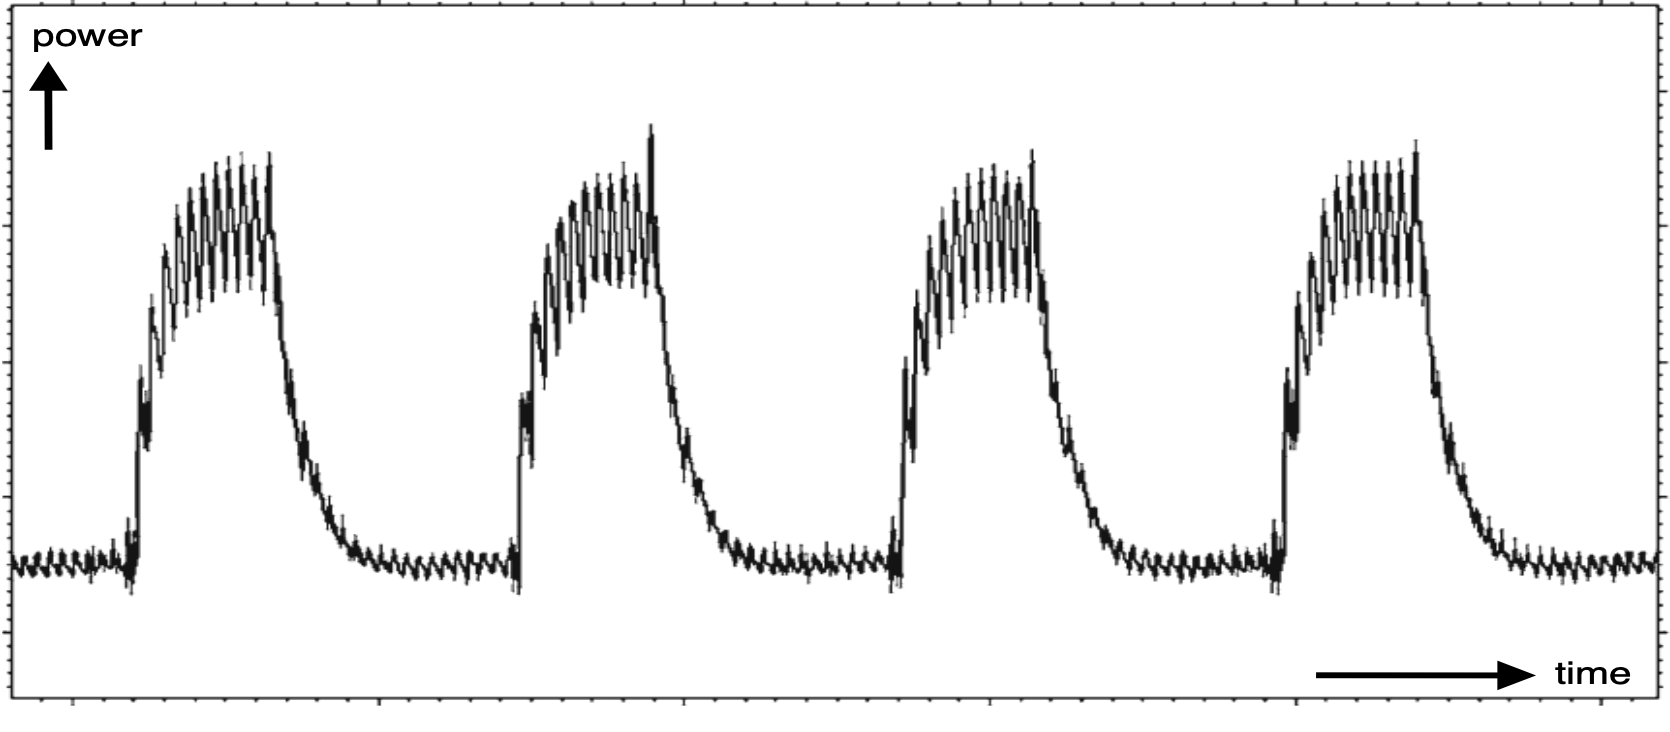
\includegraphics[width=0.4\linewidth]{figures/chapter4/fig12-a.png}
  	\label{fig:4-12-a}
  }
  \quad\quad\quad
  \subfigure[S盒LSB的输出为$0$和为$1$的情况]{
  	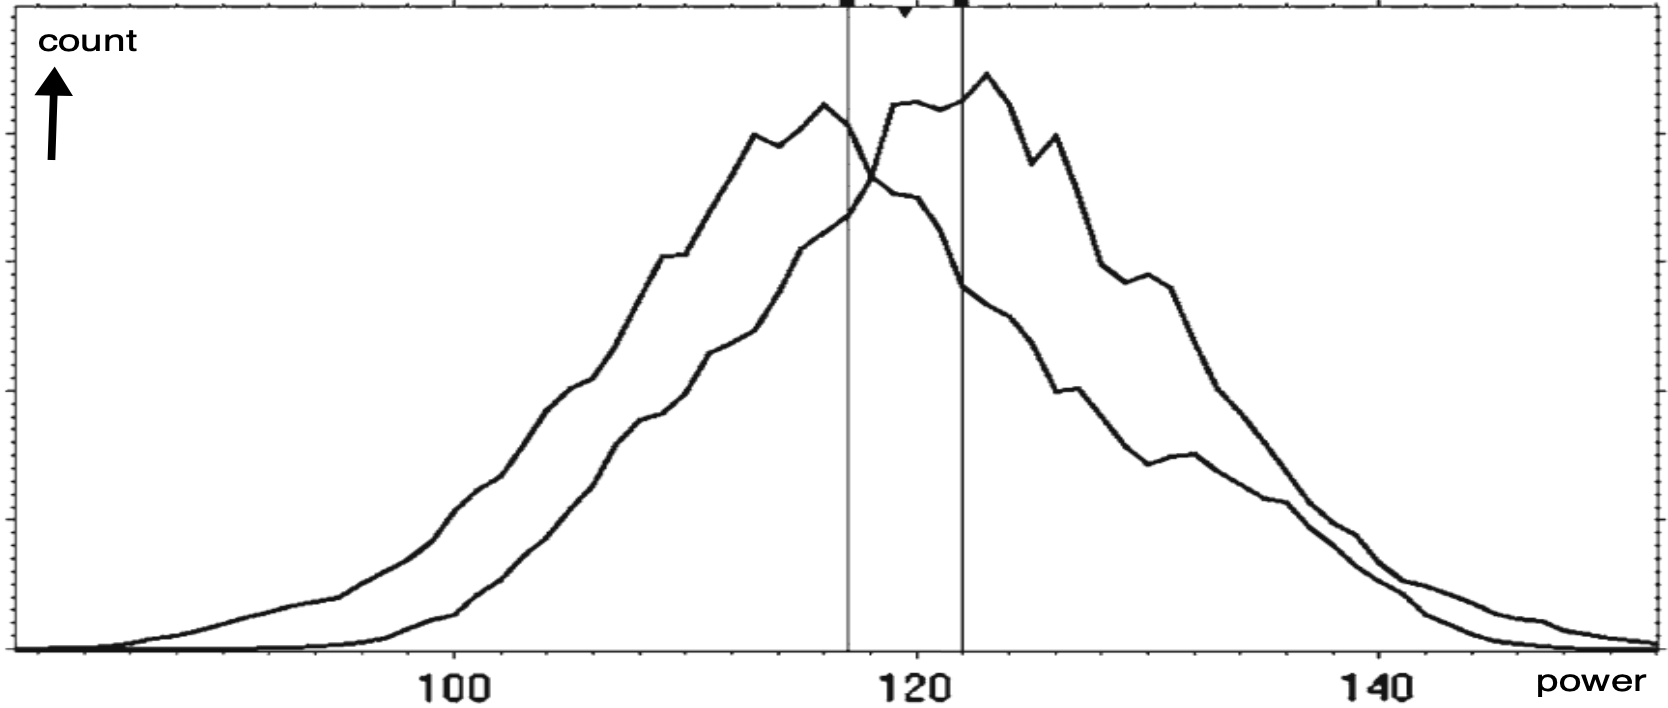
\includegraphics[width=0.4\linewidth]{figures/chapter4/fig12-b.png}
  	\label{fig:4-12-b}
  }
  
  \subfigure[功耗差分]{
  	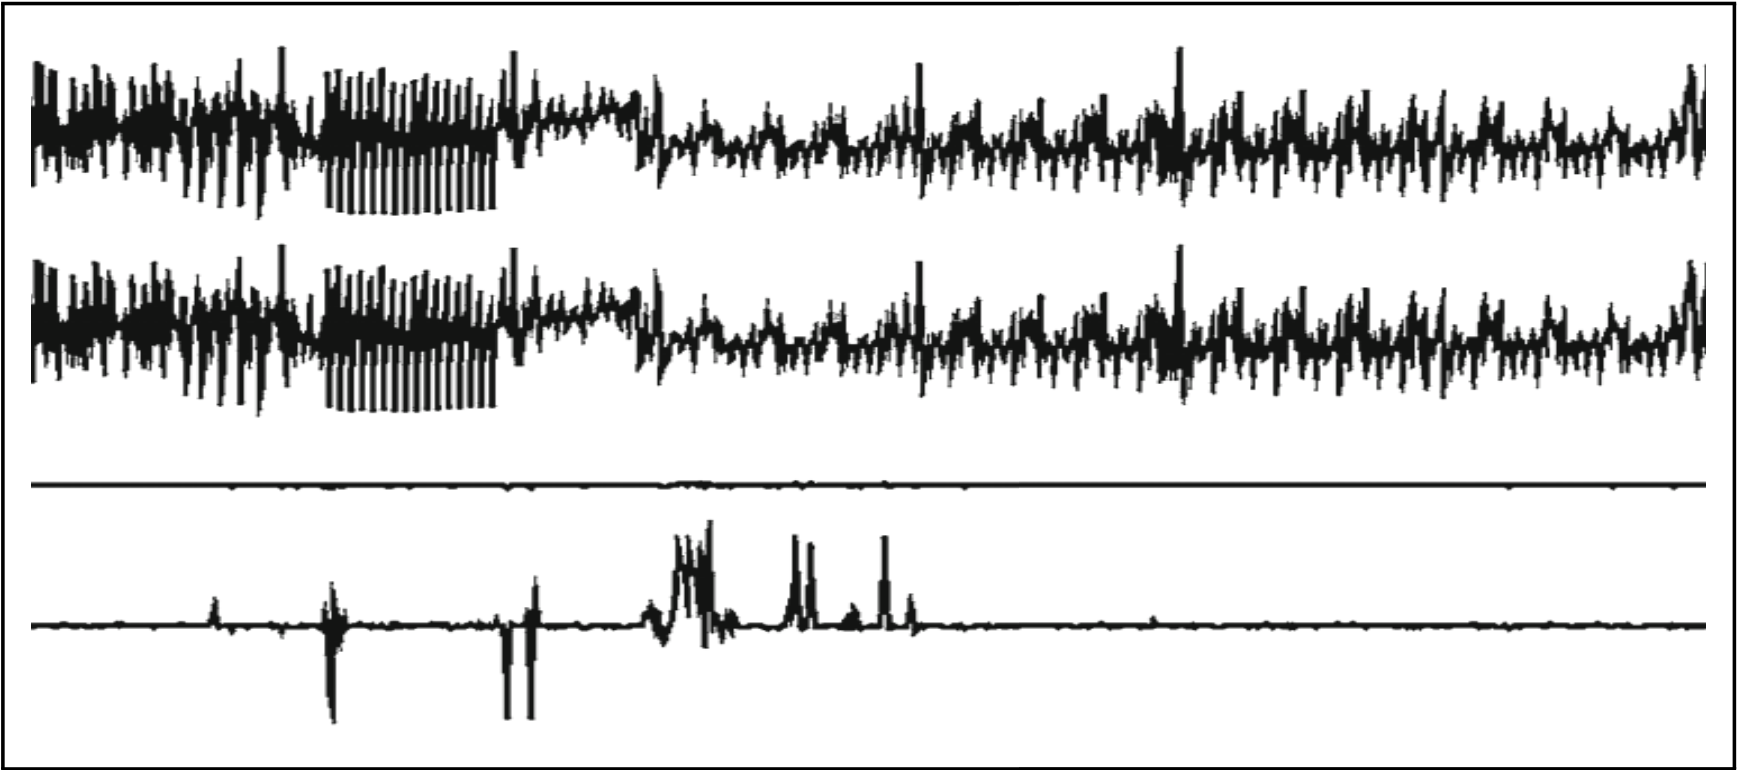
\includegraphics[width=0.4\linewidth]{figures/chapter4/fig12-c.png}
  	\label{fig:4-12-c}
  }
  \quad\quad\quad
  \subfigure[密钥$k=101,\dots,105$时的差分]{
  	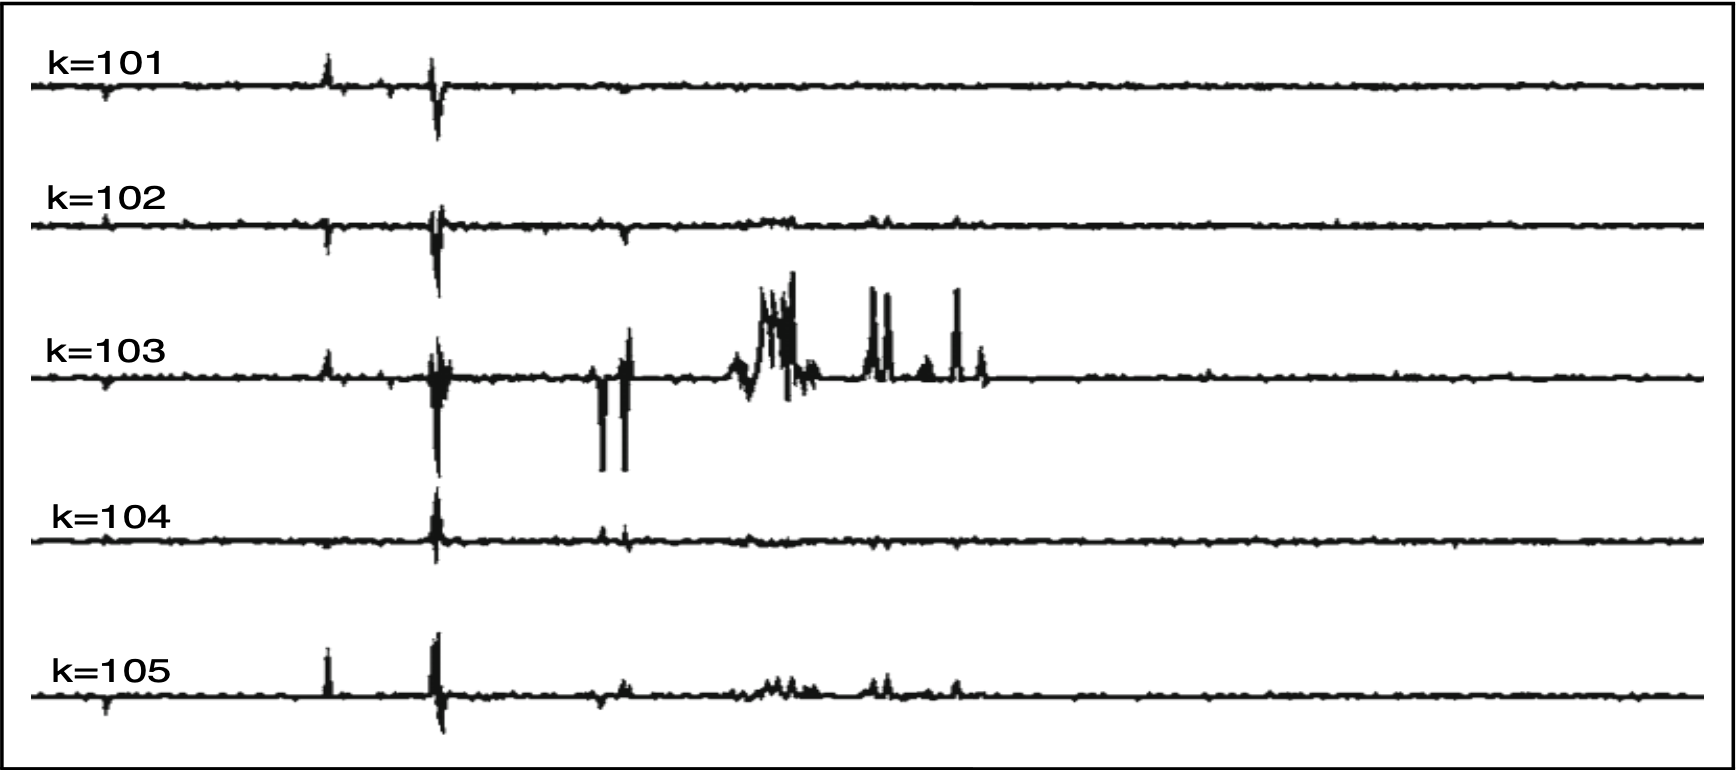
\includegraphics[width=0.4\linewidth]{figures/chapter4/fig12-d.png}
  	\label{fig:4-12-d}
  }
  \caption{针对AES的功耗分析}
\end{figure}

\begin{snote}[差分功耗分析。]
尽管 AES 对简单功耗攻击有抵抗能力,但一种更复杂的功耗攻击就能从一些简陋的 AES 算法实现中提取出 AES 密钥。随机选择一个 AES 密钥 $k$,并用它加密 $4000$ 条随机的明文。对于我们的测试设备来说,所产生的 $4000$ 个功耗轨迹图看起来非常不同,这表明在输入是随机明文的情况下,功耗轨迹与输入是相关的。

接下来,考虑第一轮中第一个 S 盒的输出,我们把这个输出称为 $T$。我们假设,S 盒查询的功耗取决于被查询的位置。也就是说,我们猜测 $T$ 的值与查表操作的功耗相关。

为了验证这个假设,我们根据 $T$ 的最小有效比特将 $4000$ 次的功率轨迹图分成两堆,第 $1$ 堆中 $T$ 的最小有效比特都为 $1$,第 $0$ 堆中 $T$ 的最小有效比特都为 $0$。考察加密信用卡在计算第一个 S 盒的输出时,每堆的功耗情况:
\begin{itemize}
	\item 第 $1$ 堆 (LSB $=1$):平均功耗 $116.9$ 个单位,标准差为 $10.7$
	\item 第 $0$ 堆 (LSB $=0$):平均功耗 $121.9$ 个单位,标准差为 $9.7$
\end{itemize}
图 \ref{fig:4-12-b} 展示了这两种功耗分布。这两个分布很接近,但有明显的不同。因此,只要有足够多的独立样本,我们就可以将两种分布区别开来。

为了利用这一观察,我们考察图 \ref{fig:4-12-c}。图中的第一行显示的是第 $1$ 堆中所有功耗轨迹的平均功耗情况。第二行显示的是第 $0$ 堆中所有功耗轨迹的平均功耗情况。最下面一行表示两条平均功耗轨迹的差分。我们可以发现,差分轨迹的第一个尖峰恰好位于计算第一个 S 盒输出时,而该尖峰的大小与图 \ref{fig:4-12-b} 中所显示的平均数之差完全对应。我们将这条差分轨迹称为\textbf{功耗差分 (power differential)}。

为了攻击目标设备,攻击者必须首先用一个干净的设备进行实验:攻击者将选定的密钥加载到设备中,并计算出设备的功耗差分轨迹,如图 \ref{fig:4-12-b} 所示。接下来,假设攻击者获得了一个带有未知的嵌入式密钥的设备,它就可以用以下方法提取密钥:
 
\vspace*{5pt}

\hspace*{5pt} 首先,对 $4000$ 条随机明文测量加密操作的功耗轨迹\\
\hspace*{26pt} 然后,对密钥首字节的每个候选值 $k\in\{0,1\}^8$,进行如下操作:\\
\hspace*{50pt} 根据 $T$ 的首个比特将 $4000$ 个样本分成两堆\\
\hspace*{75pt} (这是用目前对 $k$ 的猜测和 $4000$ 个已知的明文完成的)\\
\hspace*{50pt} 如果得到的功率差分轨迹与预先计算的曲线相匹配:\\
\hspace*{75pt} 输出 $k$ 作为密钥的首字节并停机

\vspace*{5pt}

\noindent
图 \ref{fig:4-12-d} 展示了这种攻击的效果。当使用密钥首字节的正确值(即 $k=103$)时,我们就能得到正确的功耗差分轨迹。而当使用错误的猜测($k=101,102,104,105$ 等)时,功耗差分与预期的轨迹不相符。

对 AES-128 密钥的所有 $16$ 个字节反复进行这一操作,就可以恢复整个密钥。
\end{snote}

\begin{snote}[缓和措施。]
针对功耗分析的一个常见的防御措施是进行硬件微调。从概念上讲,在执行 AES 之前,硬件会抽取固定数量的电力给电容器充电,然后利用电容器中的电力运行整个 AES 算法。一旦 AES 完成,留在电容器中的多余电量就会被丢弃。下一次应用 AES 时会再次给电容器充电,如此反复。这种概念设计(在实践中正确地实施需要一定程度的工作)旨在确保设备的功耗与设备中嵌入的密钥完全无关。

另一种缓和措施承认,每次运行解密算法都会泄露关于密钥的一些有限信息。这种措施提出在每次调用算法后重新随机化密钥,这样攻击者就不能将他从每次执行中获取到的信息结合起来。这种方法在一个被称为\textbf{抗泄露密码学 (leakage-resilient cryptography)}的领域中得到了广泛的研究。
\end{snote}

\subsection{针对AES的错误注入攻击}\label{subsec:4-3-3}

另一类攻击称为\textbf{错误注入攻击 (fault injection attack)},它试图故意在硬件运行密码系统时引入错误。攻击者可以利用畸形的输出来了解有关密钥的信息。注入错误可以通过对目标硬件进行超频,用激光加热,或对目标芯片进行电磁干扰来实现。

错误注入攻击已经被用来破解脆弱的 AES 实现,方法是迫使AES引擎在加密一个明文分组时发生故障。由此产生的畸变密文可以揭示有关密钥的信息。错误注入攻击也常被用在公钥密码场景中,我们将在 \ref{sec:17-6} 节回来详细地讨论它们,在那里,我们将介绍使用错误注入攻击完全破解 RSA 的一些实现的方法。

对错误注入攻击的一种防御措施是检查计算的结果。例如,AES 算法可以检查计算出的密文在解密后能否还原到给定的明文。如果检查失败,硬件就会抛出一个错误,并丢弃计算出的密文。但这种措施会将 AES 的性能降至原先的一半,因此不适合在实践中使用。

\subsection{量子穷举搜索攻击}\label{subsec:4-3-4}

到目前为止,我们描述的攻击都工作在经典计算机上。然而我们的物理世界是由量子力学定律所支配的。从理论上讲,人类可以构建基于量子力学定律的计算机,而这种计算机的计算能力要远超现在的经典计算机。尽管目前还没有人成功建造量子计算机,但第一台量子计算机的建成可能只是一个时间问题。

量子计算机对密码学有重大影响,因为它们可以被用来加速某些攻击,甚至完全打破一些系统。回顾一下,在经典的穷举搜索中,攻击者会得到一些用某个密钥 $k\in\mathcal{K}$ 创建的明文/密文对。攻击者会尝试所有的密钥,直到他找到一个能将给定的明文映射到给定的密文的密钥。在一台经典计算机上,这需要的时间与 $|\mathcal{K}|$ 成正比。


\begin{snote}[量子穷举搜索。]
令人惊讶的是,在量子计算机上,同样的穷举搜索的耗时只与 $\sqrt{|\mathcal{K}|}$ 成正比。这意味着对于像 AES-128 这样的分组密码,穷举搜索只需要大约 $\sqrt{2^{128}}=2^{64}$ 次计算。而使用经典计算机已经可以在合理的时间内完成 $2^{64}$ 步的计算,所以一旦量子计算机建成,它们也将能够进行这种规模的计算。因此,一旦量子计算机被制造出来,AES-128 将被认为是不安全的。

上述讨论表明,一个分组密码想要抵御量子穷举搜索攻击,其密钥空间 $|\mathcal{K}|$ 必须至少有 $2^{256}$ 那么大。此时,量子穷举搜索的时间是 $2^{128}$ 数量级的。量子计算机的这种威胁是 AES 支持 $256$ 比特密钥的原因之一。当然,我们不能保证没有更快的量子算法来破解 AES-256,但至少量子穷举搜索是不可能的。
\end{snote}

\begin{snote}[格罗弗算法。]
量子穷举搜索算法是量子计算中一个更一般结论的特例,该结论由洛夫·格罗弗 (Lov Grover) 提出。该结论表明:假设我们有一个函数 $f:\mathcal{K}\to\{0,1\}$,对于某个 $k_0\in\mathcal{K}$,$f$ 的定义如下:
\begin{equation}\label{eq:4-20}
f(k)=\left\{
\begin{array}{ll}
1, & k=k_0\\
0, & k\neq k_0
\end{array}
\right.
\end{equation}
我们的目标是在只能黑箱访问 $f$(即只能在不同的输入情况下查询$f$的输出)的情况下找到 $k_0$。在经典计算机上,没有任何其他方法的效率高于穷举所有的 $k\in\mathcal{K}$,在最糟糕的情况下,这需要对 $f$ 进行 $|\mathcal{K}|$ 数量级的查询。

格罗弗算法表明,在量子计算机上只需 $O\big(\sqrt{|K|}\cdot{\rm time}(f)\big)$ 步就可以找到 $k_0$,其中 ${\rm time}(f)$ 表示计算 $f(x)$ 的耗时。这是个结论是普适的,它对任何形如式 \ref{eq:4-20} 的函数 $f$ 都成立。该结论可以用于加速一般的硬优化问题,是量子计算机的杀手锏。

在给定若干明文/密文对的情况下,为了破解一个像 AES-128 这样的分组密码,我们定义函数:
\[
f_{\rm AES}(k)=\left\{
\begin{array}{ll}
1, & {\rm AES}(k,\overline m)=\bar c\\
0, & {\rm AES}(k,\overline m)\neq\bar c
\end{array}
\right.
\]
其中 $\overline m=(m_0,\dots,m_Q)$,$\bar c=(c_0,\dots,c_Q)$ 是给定的明文和密文分组。假设给定足够多的分组,则必有唯一密钥 $k_0\in\mathcal{K}$ 满足 ${\rm AES}(k_0,\overline m)=\bar c$。而格罗弗算法可以在 $\sqrt{|\mathcal{K}|}$ 数量级的时间内找到这个密钥。
\end{snote}
\section{伪随机函数:基本定义与性质}

虽然安全的分组密码是许多密码系统的组成部分,但一个与之密切相关的概念,即伪随机函数(PRF),被证明是许多应用中的正确工具。PRF在概念上比分组密码更加简单,正如我们将看到的,它们有着广泛的应用。PRF和分组密码密切相关,在某些假设下,我们可以用安全的分组密码作为安全伪随机函数的替身。这种性质非常有益,因为正如我们在上一节所看到的,我们已经有了许多非常实用的、貌似安全的分组密码。

\subsection{定义}

\textbf{伪随机函数 (Pseudo-random function, PRF)} $F$ 是一种确定性算法,它有两个输入:一个密钥 $k\in\mathcal{K}$ 和一个\textbf{输入数据分组} $x\in\mathcal{X}$;它的输出 $y:=F(k,x)\in\mathcal{Y}$ 被称为\textbf{输出数据分组}。我们称 $F$ \textbf{定义在} $(\mathcal{K},\mathcal{X},\mathcal{Y})$ \textbf{上}。

直观地讲,我们对伪随机函数的安全概念表明,对于一个随机选择的密钥 $k$,函数 $F(k,\cdot)$ 对于所有实际目的都应该是一个``看起来像"随机分布的一个从 $\mathcal{X}$ 到 $\mathcal{Y}$ 的映射。为了使这一概念更加精确,我们首先引入一些符号:
\[
{\rm Funs}[\mathcal{X},\mathcal{Y}]
\]
表示\emph{所有}函数 $f:\mathcal{X}\to\mathcal{Y}$ 构成的集合。这是一个非常大的集合,事实上:
\[
|{\rm Funs}[\mathcal{X},\mathcal{Y}]|=|\mathcal{Y}|^{|\mathcal{X}|}
\]

我们可以定义如下的攻击游戏:

\begin{game}[伪随机函数]\label{game:4-2}
对于一个给定的定义在 $(\mathcal{K},\mathcal{X},\mathcal{Y})$ 上的 PRF $F$,对于一个给定对手 $\mathcal{A}$,我们定义两个实验:实验$0$和实验$1$。对于$b=0,1$,我们定义:\\
\noindent\textbf{实验$b$:}
\begin{itemize}
	\item 挑战者按照如下方式选定 $f\in{\rm Funs}[\mathcal{X},\mathcal{Y}]$:
	\vspace{1pt}
	
	\hspace*{5pt} 如果 $b=0$:选取 $k\overset{\rm R}\leftarrow\mathcal{K}$,令 $f\leftarrow F(k,\cdot)$;\\
	\hspace*{5pt} 如果 $b=1$:选取 $f\overset{\rm R}\leftarrow{\rm Funs}[\mathcal{X},\mathcal{Y}]$。
	\item 对手向挑战者提交一连串的查询。\\
	对于 $i=1,2,\dots$,第 $i$ 次查询是一个输入数据分组 $x_i\in\mathcal{X}$。\\
	挑战者计算 $y_i\leftarrow f(x_i)\in\mathcal{Y}$,并将 $y_i$ 交给对手。
	\item 对手计算并输出一个比特 $\hat{b}\in\{0,1\}$。
\end{itemize}
对于 $b=0,1$,令 $W_b$ 为 $\mathcal{A}$ 在实验 $b$ 中输出 $1$ 的事件。我们将 $\mathcal{A}$ 相对于 $F$ 的\textbf{优势}定义为:
\begin{equation}\label{eq:4-21}
{\rm PRF\mathsf{adv}}[\mathcal{A}, F]:=
\Big\lvert
{\rm Pr}[W_0]-{\rm Pr}[W_1]
\Big\rvert
\end{equation}
如果对手 $\mathcal{A}$ 最多发出 $Q$ 次查询,我们就称 $\mathcal{A}$ 是一个 \textbf{$Q$ 次查询伪随机函数对手($Q$-query PRF adversary)}。
\end{game}

\begin{definition}[安全的 PRF]\label{def:4-2}
如果对于所有的有效对手 $\mathcal{A}$,${\rm PRF\mathsf{adv}}[\mathcal{A},F]$ 的值都可忽略不计,我们就称伪随机函数 $F$ 是\textbf{安全的}。
\end{definition}

需要再次强调,在攻击游戏 \ref{game:4-2} 中,对手所做的查询可以是自适应的:对手可以根据挑战者之前应答的内容来构造每个新的查询(见练习 \ref{exer:4-6})。

正如 \ref{subsec:2-2-5} 小节所讨论的,攻击游戏 \ref{game:4-2} 可以被重构为一个``比特猜测"游戏。在该游戏中,挑战者并不运行两个独立的实验,而是随机选择一个 $b\in\{0,1\}$,然后针对对手 $\mathcal{A}$ 运行实验 $b$。在这个游戏中,我们令 $\mathcal{A}$ 的比特猜测优势 ${\rm PRF\mathsf{adv}}^*[\mathcal{A}, F]$ 为 $|{\rm Pr}[\hat{b}=b]-{1}/{2}|$。那么,\ref{subsec:2-2-5} 小节中的推广结论(即式 \ref{eq:2-11})在此也适用:
\begin{equation}
{\rm PRF\mathsf{adv}}[\mathcal{A}, F]=2\cdot {\rm PRF\mathsf{adv}}^*[\mathcal{A}, F]
\end{equation}

\begin{snote}[弱安全的伪随机函数。]
对于某些使用 PRF 的构造来说,PRF 满足比定义 \ref{def:4-2} 更弱的安全属性也就足够了。我们说,如果对手的查询受到严格限制,但仍没有有效对手能够将 PRF 与随机函数区分开来时,我们就说该 PRF 是\emph{弱安全的}。所谓的查询的严格限制,指的是对手只能在域中的\emph{随机}点上查询函数。将对手的查询限制在随机输入上,就有可能更容易建立弱安全的 PRF。在练习 \ref{exer:4-2} 中,我们会研究弱安全但不完全安全的自然 PRF 构造。

我们通过稍微修改攻击游戏 \ref{game:4-2} 来定义弱安全的 PRF。假设 $F$ 是一个定义在 $(\mathcal{K},\mathcal{X},\mathcal{Y})$ 上的 PRF。现在,我们修改对手 $\mathcal{A}$ 与挑战者的交互方式:每当对手 $\mathcal{A}$ 查询函数时,挑战者都选择一个随机数 $x\in\mathcal{X}$,并将 $x$ 与 $f(x)$ 都发送给对手。换句话说,对手 $\mathcal{A}$ 看到的是函数 $f$ 在 $\mathcal{X}$ 上的一个\emph{随机}点上的评估结果,并且需要判断该函数是真正的随机函数还是一个伪随机函数。我们将对手 $\mathcal{A}$ 在该游戏中的优势定义为 ${\rm wPRF\mathsf{adv}}[\mathcal{A}, F]$,如式 \ref{eq:4-21} 所示。
\end{snote}

\begin{definition}[弱安全的 PRF]\label{def:4-3}
如果对于所有的有效对手 $\mathcal{A}$, ${\rm wPRF\mathsf{adv}}[\mathcal{A}, F]$ 的值都可忽略不计,我们就称伪随机函数 $F$ 是\textbf{弱安全的}。
\end{definition}

\subsection{随机函数的有效实现}\label{subsec:4-4-2}

同 \ref{subsec:4-1-2} 小节一样,我们可以通过一个\textbf{忠实的侏儒}来实现攻击游戏 \ref{game:4-2} 的实验 $1$ 中挑战者使用的从 ${\rm Funs}[\mathcal{X},\mathcal{Y}]$ 中选出的随机函数。同分组密码的情况一样,挑战者会跟踪输入/输出对 $(x_i,y_i)$。当挑战者收到第 $i$ 次查询 $x_i$ 时,它需要验证是否存在某个 $j < i$ 使得 $x_i=x_j$ 成立。如果存在,它就令 $y_i\leftarrow y_j$(这确保挑战者确实实现了一个函数),否则就从集合 $\mathcal{Y}$ 中随机选择一个 $y_i$;最后,挑战者将 $y_i$ 发送给对手。我们可以把挑战者的这种实现逻辑表述如下:

\vspace{5pt}

\hspace*{5pt} 当从对手 $\mathcal{A}$ 处收到第 $i$ 个查询 $x_i\in\mathcal{X}$ 时:\\
\hspace*{50pt} 如果存在某个 $j<i$ 使得 $x_i=x_j$ 成立:\\
\hspace*{75pt} 令 $y_i\leftarrow y_j$\\
\hspace*{75pt} 否则,选取 $y_i\overset{\rm R}\leftarrow\mathcal{Y}$\\
\hspace*{50pt} 将 $y_i$ 发送给 $\mathcal{A}$。\\

\subsection{什么时候一个安全的分组密码是安全的PRF?}

在本小节的开始,我们提出一个问题:什么时候一个安全分组密码才是一个安全的 PRF?在回答这个问题时,我们要介绍一种在整个密码学中被大量使用的证明技术。

令 $\mathcal{E}=(E,D)$ 是一个定义在 $(\mathcal{K},\mathcal{X})$ 上的分组密码,并令 $N:=|\mathcal{X}|$。我们可以自然地把 $\mathcal{E}$ 看作是一个定义在 $(\mathcal{K},\mathcal{X},\mathcal{X})$ 上的 PRF。现在假设 $\mathcal{E}$ 是一个安全分组密码,也就是说,不存在有效对手能够有效地将 $\mathcal{E}$ 与随机置换区分开来。这是否意味着 $\mathcal{E}$ 也是一个安全的 PRF 呢?也即,这是否意味着不存在有效对手可以有效地将 $\mathcal{E}$ 与随机函数区分开来?

这个问题的答案是``是",前提是 $N$ 是超多项式的。在论证这个问题之前,我们需要先论证,当 $N$ 很小的时候,上述问题的答案``否"。

考虑一个 PRF 对手,它对 $\mathcal{E}$ 进行攻击游戏 \ref{game:4-2} 中所描述的攻击,令 $f$ 是挑战者选择的函数:在实验 $0$ 中,$f=E(k,\cdot)$,其中 $k\in\mathcal{K}$ 为一随机值;而在实验 $1$ 中,$f$ 是从 ${\rm Funs}[\mathcal{X},\mathcal{Y}]$ 中随机选出的。假设 $N$ 是如此之小,以至于一个有效对手可以对所有的 $x\in\mathcal{X}$ 计算 $f(x)$ 的值。此外,如果对手 $\mathcal{A}$ 看到了两个不同的 $x,x'\in\mathcal{X}$ 使得 $f(x)=f(x')$,它就输出 $1$,否则就输出 $0$。显然,在实验 $0$ 中,$\mathcal{A}$ 输出 $1$ 的概率为 $0$,因为此时 $f=E(k,\cdot)$ 是一个置换。然而,在实验 $1$ 中,$\mathcal{A}$ 能以 $1-{N!}/{N^N}\geq{1}/{2}$ 的概率输出 $1$。因此我们有 ${\rm PRF\mathsf{adv}}[\mathcal{A}, F]\geq{1/2}$,所以 $\mathcal{E}$ 不是一个安全的 PRF。

上述论证可以用生日悖论来完善(见附录 \ref{sec:B-1} 节)。对于任何多项式边界的 $Q$,我们可以定义一个有效 PRF 对手 $\mathcal{A}$,它对 $\mathcal{E}$ 进行攻击游戏 \ref{game:4-2} 中的攻击,流程如下所述。对手 $\mathcal{A}$ 只需向挑战者发出 $Q$ 个不同的查询,当且仅当它能得到两个不同的值 $x,x'\in\mathcal{X}$ (从给挑战者的$Q$个值中选出)使得 $f(x)=f(x')$时,输出 $1$。同样,在实验 $0$ 中,$\mathcal{A}$ 输出 $1$ 的概率为 $0$。然而,根据定理 \ref{theo:B-1},在实验 $1$ 中,$\mathcal{A}$ 输出 $1$ 的概率至少为 $\min\{{Q(Q-1)}/{4N},0.63\}$。因此,只需进行 $O(N^{1/2})$ 次查询,对手就可以很容易地看到,置换的行为并不像是一个随机函数。

事实证明,``生日攻击"是所有对手所能达到的最好情况。当 $N$ 是超多项式的时候,这种攻击就变得不再可行了。

\begin{theorem}[PRF 切换引理]\label{theo:4-4}
令 $\mathcal{E}=(E,D)$ 是一个定义在 $(\mathcal{K},\mathcal{X})$ 上的分组密码,并令 $N:=|\mathcal{X}|$。令 $\mathcal{A}$ 是一个对手,它最多向挑战者发起 $Q$ 次查询。则有:
\[
\Big\lvert
{\rm BC\mathsf{adv}}[\mathcal{A},\mathcal{E}]-{\rm PRF\mathsf{adv}}[\mathcal{A},\mathcal{E}]
\Big\rvert
\leq{Q^2}/{2N}
\]
\end{theorem}

在证明这个定理之前,我们先导出下面的一个简单的推论。

\begin{corollary}\label{cor:4-5}
令 $\mathcal{E}=(E,D)$ 是一个定义在 $(\mathcal{K},\mathcal{X})$ 上的分组密码,并假设 $N:=|\mathcal{X}|$ 是超多项式的。那么,当且仅当 $\mathcal{E}$ 是一个安全的 PRF 时,$\mathcal{E}$ 是一个安全的分组密码。
\end{corollary}

\begin{proof}
根据定义,如果 $\mathcal{A}$ 是一个有效对手,它向挑战者发出的最大查询次数 $Q$ 是多项式边界的。因此,根据定理 \ref{theo:4-4},我们有:
\[
\Big\lvert
{\rm BC\mathsf{adv}}[\mathcal{A},\mathcal{E}]-{\rm PRF\mathsf{adv}}[\mathcal{A},\mathcal{E}]
\Big\rvert
\leq{Q^2}/{2N}
\]
由于 $N$ 是超多项式的,$Q$ 是多项式边界的,所以 $\frac{Q^2}{2N}$ 是可以忽略不计的(见事实 \ref{fact:2-6})。由此可见,当且仅当 ${\rm PRF\mathsf{adv}}[\mathcal{A},\mathcal{E}]$ 可忽略不计时,${\rm BC\mathsf{adv}}[\mathcal{A},\mathcal{E}]$ 才是可以忽略不计的。
\end{proof}

实际上,定理 \ref{theo:4-4} 的证明与分组密码和 PRF 无关,它实际上是一个关于随机置换和随机函数的论证。让我们定义一个新的攻击游戏,用以测试对手区分随机置换与随机函数的能力。

\begin{game}[置换 \emph{vs.} 函数]\label{game:4-3}
对于一个给定有限集 $\mathcal{X}$ 和一个给定对手 $\mathcal{A}$,我们定义两个实验:实验$0$和实验$1$。对于$b=0,1$,我们定义:\\
\textbf{实验$b$:}
\begin{itemize}
	\item 挑战者按照如下方式选定 $f\in{\rm Funs}[\mathcal{X},\mathcal{X}]$:
	\vspace{1pt}
	
	\hspace*{5pt} 如果 $b=0$:选取 $f\overset{\rm R}\leftarrow{\rm Perms}[\mathcal{X}]$;\\
	\hspace*{5pt} 如果 $b=1$:选取 $f\overset{\rm R}\leftarrow{\rm Funs}[\mathcal{X},\mathcal{X}]$。
	\item 对手向挑战者提交一连串的查询。\\
	对于 $i=1,2,\dots$,第 $i$ 次查询是一个输入数据分组 $x_i\in\mathcal{X}$。\\
	挑战者计算 $y_i\leftarrow f(x_i)\in\mathcal{Y}$,并将 $y_i$ 交给对手。
	\item 对手计算并输出一个比特 $\hat{b}\in\{0,1\}$。
\end{itemize}
对于 $b=0,1$,令 $W_b$ 为 $\mathcal{A}$ 在实验 $b$ 中输出 $1$ 的事件。我们将 $\mathcal{A}$ 相对于 $\mathcal{X}$ 的\textbf{优势}定义为:
\[
{\rm PF\mathsf{adv}}[\mathcal{A}, \mathcal{X}]:=
\Big\lvert
{\rm Pr}[W_0]-{\rm Pr}[W_1]
\Big\rvert
\]
\end{game}

\begin{theorem}\label{theo:4-6}
令 $\mathcal{X}$ 是一个大小为 $N$ 的有限集,$\mathcal{A}$ 是一个对手,它最多向挑战者发起 $Q$ 次查询,则有:
\[
{\rm PF\mathsf{adv}}[\mathcal{A},\mathcal{X}]\leq{Q^2}/{2N}
\]
\end{theorem}


我们首先表明,上面的定理很容易推出定理 \ref{theo:4-4}。

\begin{proof}[定理 \ref{theo:4-4} 的证明]
令 $\mathcal{E}=(E,D)$ 是一个定义在 $(\mathcal{K},\mathcal{X})$ 上的分组密码。令 $\mathcal{A}$ 是一个对手,它最多向挑战者发起 $Q$ 次查询。我们定义游戏 $0$、游戏 $1$ 和游戏 $2$,它们都在 $\mathcal{A}$ 和挑战者之间进行。对于 $j=0,1,2$,我们定义 $p_j$ 为 $\mathcal{A}$ 在游戏 $j$ 中输出 $1$ 的概率。在每个游戏中,挑战者根据特定的分布选择一个函数 $f:\mathcal{X}\to\mathcal{X}$,并以 $f(x)$ 来应答 $\mathcal{A}$ 的每个查询 $x\in\mathcal{X}$。

\noindent\textbf{游戏 $\mathbf{0}$}:该游戏中的挑战者令 $f:=E(k,\cdot)$,其中 $k\in\mathcal{K}$ 是随机选出的。

\noindent\textbf{游戏 $\mathbf{1}$}:该游戏中的挑战者随机选择 $f\in{\rm Perms}[\mathcal{X}]$。

\noindent\textbf{游戏 $\mathbf{2}$}:该游戏中的挑战者随机选择 $f\in{\rm Funs}[\mathcal{X},\mathcal{X}]$。

注意到,根据定义,有:
\[
\begin{aligned}
	& |p_1-p_0| = {\rm BC\mathsf{adv}}[\mathcal{A},\mathcal{E}]\\
	& |p_2-p_0| = {\rm PRF\mathsf{adv}}[\mathcal{A},\mathcal{E}]
\end{aligned}
\]
而根据定理 \ref{theo:4-6},有:
\[
|p_2-p_1|={\rm PF\mathsf{adv}}[\mathcal{A},\mathcal{X}]\leq{Q^2}/{2N}
\]
将上两式结合,我们得到:
\[
\big\lvert
{\rm BC\mathsf{adv}}[\mathcal{A},\mathcal{E}]-{\rm PRF\mathsf{adv}}[\mathcal{A},\mathcal{E}]
\big\rvert
=
\big\lvert
|p_1-p_0|-|p_2-p_0|
\big\rvert
\leq|p_2-p_1|\leq{Q^2}/{2N}
\]

这就证明了该定理。
\end{proof}

所以,剩下工作的就是证明定理 \ref{theo:4-6}。在此之前,我们要说明一个非常简单但非常有用的结论:

\begin{theorem}[差分引理]\label{theo:4-7}
令 $Z$,$W_0$,$W_1$ 是定义在某个概率空间上的事件。假设当且仅当 $W_1\land\bar Z$ 发生时,$W_0\land\bar Z$ 才发生,则我们有:
\[
|\Pr[W_0]-\Pr[W_1]|\leq\Pr[Z]
\]
\end{theorem}

\begin{proof}
这就是一个简单的计算。我们有:
\[
\begin{aligned}
|\Pr[W_0]-\Pr[W_1]|
&=|\Pr[W_0\land Z]+\Pr[W_0\land\bar Z]-\Pr[W_1\land Z]-\Pr[W_1\land\bar Z]|\\
&=|\Pr[W_0\land Z]-\Pr[W_1\land Z]|\\
&\leq \Pr[Z]
\end{aligned}
\]
其中第二个等式来自 $W_0\land\bar{Z} \Longleftrightarrow W_1\land\bar{Z}$ 的假设,所以,一个特殊结论就是 $\Pr[W_0\land\bar{Z}]=\Pr[W_1\land\bar{Z}]$。最后的不等式来自于这样一个事实,即 $\Pr[W_0\land Z]$ 和 $\Pr[W_1\land Z]$ 都是介于 $0$ 和 $\Pr[Z]$ 之间的值。
\end{proof}
 
在我们对差分定理的大多数应用中,$W_0$ 代表一个给定对手在对某个挑战者的游戏中输出 $1$ 的事件,而 $W_1$ 则是同一个对手在对另一个挑战者的游戏中输出 $1$ 的事件。为了应用差分定理,我们定义这两个游戏,使它们都在相同的基础概率空间上运行。这意味着我们假设对手和挑战者在两个游戏中所做的随机选择都是一样的,两个游戏的不同之处仅在于挑战者针对来自对手的查询给出反馈的策略。

\begin{proof}[定理 \ref{theo:4-6} 的证明]
考虑一个对手 $\mathcal{A}$,它对 $\mathcal{X}$ 进行攻击游戏 \ref{game:4-3} 中的攻击,其中 $N:=|\mathcal{X}|$,并假设 $\mathcal{A}$ 最多向挑战者发起 $Q$ 次查询。考虑这个攻击游戏的实验 $0$。利用 \ref{subsec:4-4-2} 小节讨论的``忠实的侏儒"的思想,我们可以通过跟踪输入/输出对 $(x_i,y_i)$ 来实现实验 $0$;此外,为 $y_i$ 选择初始的``默认"值 $z_i$ 是很方便的,$z_1,\dots,z_Q$ 可以从 $\mathcal{X}$ 中均匀独立随机选出;这些``默认"值在必要时可以被覆写,以确保挑战者定义的是一个随机置换。下面是详细的过程:

\vspace{5pt}

\hspace*{5pt} 选取 $z_1,\dots,z_Q\overset{\rm R}\leftarrow\mathcal{X}$\\
\hspace*{26pt} 当收到 $\mathcal{A}$ 的第 $i$ 个查询 $x_i$ 时:\\
\hspace*{50pt} 如果存在某个 $j<i$ 使得 $x_i=x_j$,则:\\
\hspace*{75pt} 令 $y_i\leftarrow y_j$\\
\hspace*{50pt} 否则:\\
\hspace*{75pt} 令 $y_i\leftarrow z_i$\\
\hspace*{1pt} ($*$)
\hspace*{53pt} 如果 $y_i\in\{y_1,\dots,y_{i-1}\}$,则选取 $y_i\overset{\rm R}\leftarrow\mathcal{X}\setminus\{y_1,\dots,y_{i-1}\}$;\\
\hspace*{50pt} 将 $y_i$ 发送给 $\mathcal{A}$。

\vspace{5pt}

标有 ($*$) 的那行用于测试是否需要覆盖默认值 $z_i$,确保没有任何输出值被用于两个不同的输入值。

令 $W_0$ 为 $\mathcal{A}$ 在该游戏中输出 $1$ 的事件,我们称之为游戏 $0$。

我们现在修改上述挑战者的实现,得到另一个新的游戏:

\vspace{5pt}

\hspace*{5pt} 选取 $z_1,\dots,z_Q\overset{\rm R}\leftarrow\mathcal{X}$\\
\hspace*{26pt} 当收到 $\mathcal{A}$ 的第 $i$ 个查询 $x_i$ 时:\\
\hspace*{50pt} 如果存在某个 $j<i$ 使得 $x_i=x_j$,则:\\
\hspace*{75pt} 令 $y_i\leftarrow y_j$\\
\hspace*{50pt} 否则:\\
\hspace*{75pt} 令 $y_i\leftarrow z_i$\\
\hspace*{50pt} 将 $y_i$ 发送给 $\mathcal{A}$。

\vspace{5pt}

我们所做的只是在原来的挑战者逻辑中删除了标有 ($*$) 的那行,这使得我们``忠实的侏儒"变成了一个``健忘的侏儒",它忘记了检查输出值是否存在重复。

令 $W_1$ 为 $\mathcal{A}$ 在与这个修改后的挑战者进行的游戏中输出 $1$ 的事件,我们称之为游戏 $1$。

请注意,游戏 $1$ 等同于攻击游戏 \ref{game:4-3} 的实验 $1$;特别地,$\Pr[W_1]$ 等于 $\mathcal{A}$ 在攻击游戏 \ref{game:4-3} 的实验 $1$ 中输出 $1$ 的概率。因此,我们有:
\[
{\rm PF\mathsf{adv}}[\mathcal{A},\mathcal{X}]=|\Pr[W_0]-\Pr[W_1]|
\]

我们现在应用差分引理。为此,上述两个游戏都被假设运行在相同的基础概率空间上。在这两个游戏中,对手和挑战者所做的所有随机选择都是一样的,唯一不同的是挑战者用来给出应答的规则。特别地,这意味着 $\mathcal{A}$ 的随机选择和挑战者选择的值 $z_1,\dots,z_Q$ 不仅具有相同的分布,而且在两个游戏中都是\emph{确确实实的相同值}。

定义 $Z$ 为存在某个 $i\neq j$ 使得 $z_i=z_j$ 成立的事件。现在,假设我们运行游戏 $0$ 和游戏 $1$,而事件 $Z$ 没有发生。这意味着 $z_i$ 的值都是不同的。现在,由于对手的随机选择在两个游戏中都是相同的,它在两个游戏中的第一次查询也是相同的,因此挑战者的应答在两个游戏中也是相同的。对手的第二次查询(是其随机选择和挑战者第一次应答的函数)在两个游戏中也都是一样的。由于我们假设 $Z$ 没有发生,挑战者的应答在两个游戏中是相同的。继续这个论证,我们可以看到,对手的每次查询和挑战者的每个应答在两个游戏中都是一样的,因此对手的输出在两个游戏中都是一样的。因此,如果 $Z$ 没有发生,对手在游戏 $0$ 中输出 $1$,那么它在游戏 $1$ 中也会输出 $1$。同样地,如果 $Z$ 没有发生,而对手在游戏 $1$ 中输出 $1$,那么它在游戏 $0$ 中也会输出 $1$。更简洁地说,当且仅当 $W_1\land\bar{Z}$ 发生时,我们有 $W_0\land\bar{Z}$ 发生。因此,差分引理适用于该场景,我们得到:
\[
|\Pr[W_0]-\Pr[W_1]|\leq\Pr[Z]
\]

剩下的就是确定 $\Pr[Z]$ 的上界。这可由联合约束得到:对于任意不同索引对 $(i,j)$,必有$\Pr[z_i=z_j]={1}/{N}$,由于这样的索引对至多有 ${Q^2}/{2}$ 对,因此有:
\[
\Pr[Z]\leq{Q^2}/{2N}
\]
因此该定理得证。
\end{proof}

尽管还有其他的策略可以用来证明前面的定理(见练习 \ref{exer:4-24}),但我们在上面的证明中所使用的\textbf{健忘的侏儒}技术是非常有用的,我们将在后面的文章中多次看到它。

\subsection{使用 PRF 构建 PRG}\label{subsec:4-4-4}

由一个 PRF 构造一个 PRG 是很容易的。令 $F$ 是一个定义在 $(\mathcal{K},\mathcal{X},\mathcal{Y})$ 上的 PRF,$l\geq1$ 是一个多项式边界的值,令 $x_1,\dots,x_l$ 是 $\mathcal{X}$ 中任意固定且互不相同的元素(这要求$|\mathcal{X}|\geq l$)。我们定义一个具有种子空间 $\mathcal{K}$ 和输出空间 $\mathcal{Y}^l$ 的 PRG 如下:对于 $k\in\mathcal{K}$:
\[
G(k):=
\big(
F(k,x_1),\dots,F(k,x_l)
\big)
\]

\begin{theorem}\label{theo:4-8}
如果 $F$ 是一个安全的 PRF,那么上述 PRG $G$ 就是一个安全的 PRG。
\begin{quote}
特别地,对于每一个就 $G$ 进行攻击游戏 \ref{game:3-1} 的 PRG 对手 $\mathcal{A}$,都存在一个就 $F$ 进行攻击游戏 \ref{game:4-2} 的 PRF 对手 $\mathcal{B}$,其中 $\mathcal{B}$ 是一个围绕 $\mathcal{A}$ 的基本包装器,满足:
\end{quote}
\[
\mathrm{PRG}\mathsf{adv}[\mathcal{A},G]= 
\mathrm{PRF}\mathsf{adv}[\mathcal{B},F]
\]
\end{theorem}

\begin{proof}
令 $\mathcal{A}$ 是一个有效 PRG 对手,它对 $G$ 进行攻击游戏 \ref{game:3-1} 中的攻击。我们描述一个相应的 PRF 对手 $\mathcal{B}$,它对 $F$ 进行攻击游戏 \ref{game:4-2} 中的攻击。对手 $\mathcal{B}$ 的工作方式如下:
\begin{quote}
$\mathcal{B}$ 向它的挑战者发起查询 $x_1,\dots,x_\ell$ 并获得应答 $y_1,\dots,y_\ell$。然后,对手 $\mathcal{B}$ 扮演 $\mathcal{A}$ 的挑战者的角色,向 $\mathcal{A}$ 发送 $(y_1,\dots,y_\ell)$。最后,对手 $\mathcal{B}$ 原样输出 $\mathcal{A}$ 所输出的所有东西。
\end{quote}

从构造上看,对于 $b=0,1$,$\mathcal{B}$ 在攻击游戏 \ref{game:4-2} 的实验 $b$ 相对于 $F$ 输出 $1$ 的概率恰好等于 $\mathcal{A}$ 在攻击游戏 \ref{game:3-1} 的实验 $b$ 相对于 $G$ 输出 $1$ 的概率,因此定理立即得证。
\end{proof}

\subsubsection{确定性计数器模式}

上述构造为我们提供了另一种从安全分组密码中建立语义安全密码的方法。假设 $\mathcal{E}=(E,D)$ 是一个定义在 $(\mathcal{K},\mathcal{X})$ 上的分组密码,其中 $\mathcal{X}=\{0,1\}^n$。令 $N:=|\mathcal{X}|=2^n$,假设 $N$ 是超多项式的,并且 $\mathcal{E}$ 是一个安全的分组密码。那么根据定理 \ref{theo:4-4},加密函数 $\mathcal{E}$ 是一个定义在 $(\mathcal{K},\mathcal{X},\mathcal{X})$ 上的安全 PRF。然后我们可以将定理 \ref{theo:4-8} 应用于 $\mathcal{E}$  以得到一个安全 PRG,最后将定理 \ref{theo:3-1} 应用于这个 PRG,最终得到一个语义安全的流密码。

让我们详细考察这个流密码。这个密码 $\mathcal{E}'=(E',D')$ 具有密钥空间 $\mathcal{K}$ 以及消息和密文空间 $\mathcal{X}^{\leq\ell}$,其中 $\ell$ 是一个多项式边界的值,特别是 $\ell\leq N$。我们可以将 $x_1,\dots,x_\ell$ 定义为 $\mathcal{X}$ 上任何方便的元素;特别地,我们可以把 $x_i$ 定义为 $i-1$ 的 $n$ 比特二进制编码,我们将其表示为 $\langle i-1\rangle_n$。则 $\mathcal{E}'$ 的加密和解密流程如下:
\begin{itemize}
	\item 对于 $k\in\mathcal{K}$ 和 $m\in\mathcal{X}^{\leq l}$,记 $v:=|m|$,我们定义:
	\[
	E'(k,m)=(E(k,\langle0\rangle_n)\oplus m[0],\dots,E(k,\langle v-1\rangle_n)\oplus m[v-1])
	\]
	\item 对于 $k\in\mathcal{K}$ 和 $c\in\mathcal{X}^{\leq l}$,记 $v:=|c|$,我们定义:
	\[
	D'(k,c)=(E(k,\langle0\rangle_n)\oplus c[0],\dots,E(k,\langle v-1\rangle_n)\oplus c[v-1])
	\]
\end{itemize}

分组密码的这种操作模式被称为\textbf{确定性计数器模式 (deterministic couter mode)},如图 \ref{fig:4-13} 所示。与 ECB 模式不同,该模式中,解密算法 $D$ 从未被使用。将定理 \ref{theo:4-4},定理 \ref{theo:4-8} 和定理 \ref{theo:3-1} 结合起来,我们可以看到,密码 $\mathcal{E}'$ 是语义安全的;特别地,对于任何有效的语义安全对手 $\mathcal{A}$,都存在一个有效分组密码对手 $\mathcal{B}$,满足:
\begin{equation}\label{eq:4-23}
{\rm SS\mathsf{adv}}[\mathcal{A},\mathcal{E}']\leq2\cdot{\rm BC\mathsf{adv}}[\mathcal{B},\mathcal{E}]+{\ell^2}/{N}
\end{equation}

显然,确定性计数器模式相比 ECB 模式的优势在于它在是语义安全的,而且不需要对消息空间做出任何限制。唯一的缺点是,由于式 \ref{eq:4-23} 中存在 ${\ell^2}/{N}$ 项,对于非常长的消息,它的安全性可能会大大降低。因此,限制 ${\ell^2}/{2N}$ 的大小是非常重要的。考虑以下对 $\mathcal{E}'$ 的攻击。设 $m_0$ 为由 $\ell$ 个零分组组成的消息,$m_1$ 为由 $\ell$ 个随机分组组成的消息。如果攻击游戏 \ref{game:2-1} 中的挑战者使用 $\mathcal{E}'$ 对 $m_0$ 进行加密,那么密文将不包含任何重复分组。然而,根据生日悖论(见定理 \ref{theo:B-1}),如果挑战者加密 $m_1$,那么密文包含重复分组的概率至少为 $\min\{{\ell(\ell-1)}/{4N},0.63\}$。因此,以这种方式构造 $m_0$ 和 $m_1$,并在且仅在密文包含重复分组时输出 $1$ 的对手 $\mathcal{A}$,其优势随 $\ell$ 二次增长,且在 $\ell\approx N^{1/2}$ 时不可忽略不计。

\begin{figure}
  \centering
  \subfigure[加密]{\tikzset{every picture/.style={line width=0.75pt}}

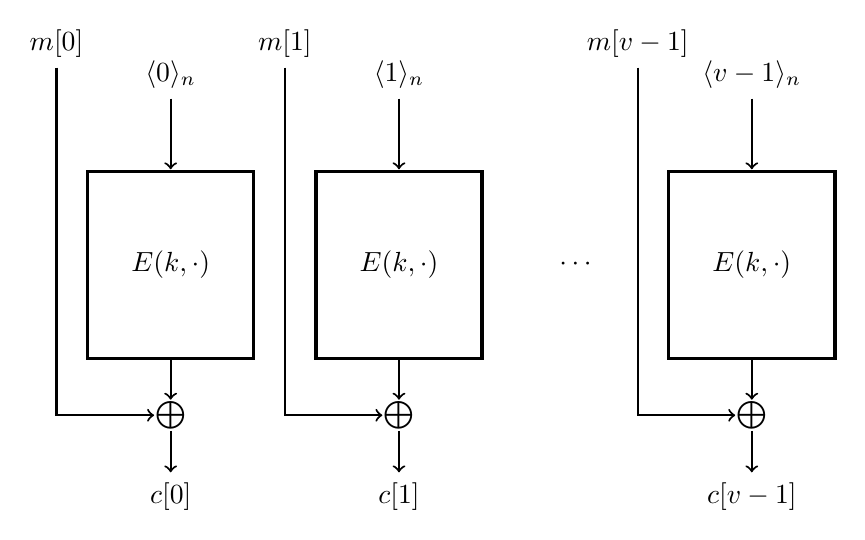
\begin{tikzpicture}[x=0.75pt,y=0.75pt,yscale=-1,xscale=1]

\draw  [line width=1.2]  (30,80) -- (110,80) -- (110,170) -- (30,170) -- cycle ;
\draw  [line width=1.2]  (140,80) -- (220,80) -- (220,170) -- (140,170) -- cycle ;
\draw  [line width=1.2]  (310,80) -- (390,80) -- (390,170) -- (310,170) -- cycle ;

\draw  [->]  (70,45) -- (70,79) ;
\draw  [->]  (180,45) -- (180,79) ;
\draw  [->]  (350,45) -- (350,79) ;
\draw  [->]  (70,170) -- (70,190) ;
\draw  [->]  (70,205) -- (70,225) ;
\draw  [->]  (180,170) -- (180,190) ;
\draw  [->]  (180,205) -- (180,225) ;
\draw  [->]  (350,170) -- (350,190) ;
\draw  [->]  (350,205) -- (350,225) ;
\draw  [->]  (15,30) -- (15,197.5) -- (62,197.5) ;
\draw  [->]  (125,30) -- (125,197.5) -- (172,197.5) ;
\draw  [->]  (295,30) -- (295,197.5) -- (342,197.5) ;

\draw (70,125) node    {$E( k,\cdot )$};
\draw (15,26.6) node [anchor=south] [inner sep=0.75pt]    {$m[ 0]$};
\draw (70.03,228.4) node [anchor=north] [inner sep=0.75pt]    {$c[ 0]$};
\draw (180,125) node    {$E( k,\cdot )$};
\draw (125,26.6) node [anchor=south] [inner sep=0.75pt]    {$m[ 1]$};
\draw (180,228.4) node [anchor=north] [inner sep=0.75pt]    {$c[ 1]$};
\draw (350,125) node    {$E( k,\cdot )$};
\draw (295,26.6) node [anchor=south] [inner sep=0.75pt]    {$m[ v-1]$};
\draw (350,228.4) node [anchor=north] [inner sep=0.75pt]    {$c[ v-1]$};
\draw (265,125) node    {$\cdots $};
\draw (70,197.5) node    {$\bigoplus $};
\draw (180,197.5) node    {$\bigoplus $};
\draw (350,197.5) node    {$\bigoplus $};
\draw (70,41.6) node [anchor=south] [inner sep=0.75pt]    {$\langle 0\rangle _{n}$};
\draw (180,41.6) node [anchor=south] [inner sep=0.75pt]    {$\langle 1\rangle _{n}$};
\draw (350,41.6) node [anchor=south] [inner sep=0.75pt]    {$\langle v-1\rangle _{n}$};

\end{tikzpicture}}
  
  \,
  
  \,
  
  \subfigure[解密]{\tikzset{every picture/.style={line width=0.75pt}}

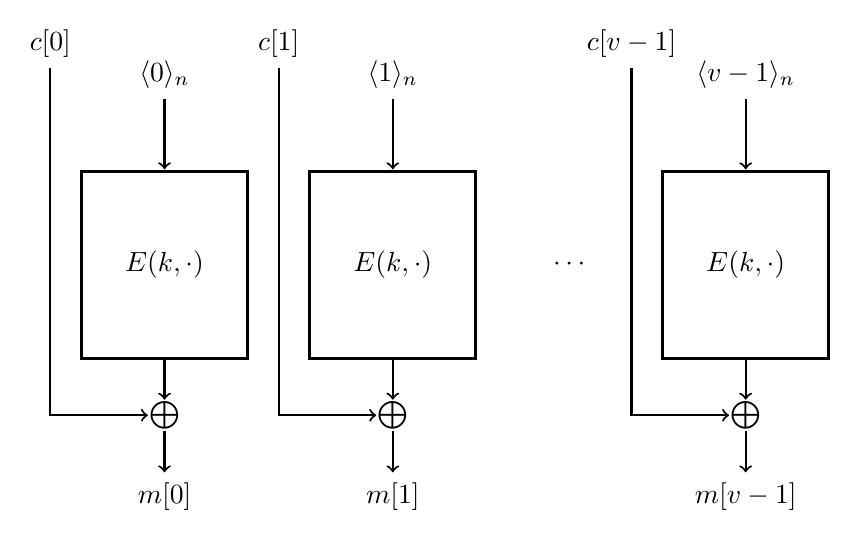
\begin{tikzpicture}[x=0.75pt,y=0.75pt,yscale=-1,xscale=1]

\draw  [line width=1.2]  (30,80) -- (110,80) -- (110,170) -- (30,170) -- cycle ;
\draw  [line width=1.2]  (140,80) -- (220,80) -- (220,170) -- (140,170) -- cycle ;
\draw  [line width=1.2]  (310,80) -- (390,80) -- (390,170) -- (310,170) -- cycle ;

\draw  [->]  (70,45) -- (70,79) ;
\draw  [->]  (180,45) -- (180,79) ;
\draw  [->]  (350,45) -- (350,79) ;
\draw  [->]  (70,170) -- (70,190) ;
\draw  [->]  (70,205) -- (70,225) ;
\draw  [->]  (180,170) -- (180,190) ;
\draw  [->]  (180,205) -- (180,225) ;
\draw  [->]  (350,170) -- (350,190) ;
\draw  [->]  (350,205) -- (350,225) ;
\draw  [->]  (15,30) -- (15,197.5) -- (62,197.5) ;
\draw  [->]  (125,30) -- (125,197.5) -- (172,197.5) ;
\draw  [->]  (295,30) -- (295,197.5) -- (342,197.5) ;

\draw (70,125) node    {$E( k,\cdot )$};
\draw (15,26.6) node [anchor=south] [inner sep=0.75pt]    {$c[ 0]$};
\draw (70.03,228.4) node [anchor=north] [inner sep=0.75pt]    {$m[ 0]$};
\draw (180,125) node    {$E( k,\cdot )$};
\draw (125,26.6) node [anchor=south] [inner sep=0.75pt]    {$c[ 1]$};
\draw (180,228.4) node [anchor=north] [inner sep=0.75pt]    {$m[ 1]$};
\draw (350,125) node    {$E( k,\cdot )$};
\draw (295,26.6) node [anchor=south] [inner sep=0.75pt]    {$c[ v-1]$};
\draw (350,228.4) node [anchor=north] [inner sep=0.75pt]    {$m[ v-1]$};
\draw (265,125) node    {$\cdots $};
\draw (70,197.5) node    {$\bigoplus $};
\draw (180,197.5) node    {$\bigoplus $};
\draw (350,197.5) node    {$\bigoplus $};
\draw (70,41.6) node [anchor=south] [inner sep=0.75pt]    {$\langle 0\rangle _{n}$};
\draw (180,41.6) node [anchor=south] [inner sep=0.75pt]    {$\langle 1\rangle _{n}$};
\draw (350,41.6) node [anchor=south] [inner sep=0.75pt]    {$\langle v-1\rangle _{n}$};

\end{tikzpicture}}
  \caption{确定性计数器模式的加密和解密}
  \label{fig:4-13}
\end{figure}

\subsection{数学细节}

同之前一样,我们使用 \ref{sec:2-3} 中定义的术语对 PRF 给出一个更精确的数学定义。

\begin{definition}[伪随机函数]
一个\textbf{伪随机函数}包含一个算法 $F$,以及三个具有系统参数化 $P$ 的空间族:
\[
\mathbf{K}=\{\mathcal{K}_{\lambda,\Lambda}\}_{\lambda,\Lambda},\quad
\mathbf{X}=\{\mathcal{X}_{\lambda,\Lambda}\}_{\lambda,\Lambda},\quad
\mathbf{Y}=\{\mathcal{Y}_{\lambda,\Lambda}\}_{\lambda,\Lambda}
\]
它们满足:
\begin{enumerate}
	\item $\mathbf{K}$,$\mathbf{X}$ 和 $\mathbf{Y}$ 是可有效识别的。
	\item $\mathbf{K}$ 和 $\mathbf{Y}$ 是可有效采样的。
	\item 算法 $F$ 是一个确定性算法,对于输入 $\lambda\in\mathbb{Z}_{\geq1}$,$\Lambda\in{\rm Supp}(P(\lambda))$,$k\in\mathcal{K}_{\lambda,\Lambda}$ 和 $x\in\mathcal{X}_{\lambda,\Lambda}$,其运行时间以 $\lambda$ 的一个多项式为界,并且输出 $\mathcal{Y}_{\lambda,\Lambda}$ 中的一个元素。
\end{enumerate}
\end{definition}
和之前一样,在定义安全性时,攻击游戏是由安全参数和系统参数决定的,而优势是安全参数的一个函数。
\section{使用 PRF 构建分组密码}\label{sec:4-5}

在本节中,我们将展示如何基于任何安全的 PRF 构建一个安全的分组密码,其输入空间和输出空间都是 $\{0,1\}^n$,其中 $2^n$ 是超多项式的。该构造被称为卢比-拉克福(Luby-Rackoff)构造。该结论本身主要具有理论意义,因为实践中通常使用另一种更特别的方式来构造分组密码;然而,这个结论有时候会被看作是一些实际的分组密码被设计成费斯妥网络的理由(见 \ref{subsec:4-2-1} 小节)。

令 $F$ 是一个定义在 $(\mathcal{K},\mathcal{X},\mathcal{X})$ 上的 PRF,其中 $\mathcal{X}=\{0,1\}^n$。我们下面构造一个分组密码 $\mathcal{E}=(E,D)$,其密钥空间为 $\mathcal{K}^3$,数据分组空间为 $\mathcal{X}^2$。

给定一个密钥 $(k_1,k_2,k_3)\in\mathcal{K}^3$ 和一个数据分组 $(u,v)\in\mathcal{X}^2$,加密算法 $E$ 运行如下:

\vspace{5pt}

\hspace*{5pt} $w\leftarrow u\oplus F(k_1,v)$\\
\hspace*{26pt} $x\leftarrow v\oplus F(k_2,w)$\\
\hspace*{26pt} $y\leftarrow w\oplus F(k_3,x)$\\
\hspace*{26pt} 输出 $(x,y)$

\vspace{5pt}

\noindent
给定一个密钥 $(k_1,k_2,k_3)\in\mathcal{K}^3$ 和一个密文分组 $(x,y)\in\mathcal{X}^2$,解密算法 $D$ 运行如下:

\vspace{5pt}

\hspace*{5pt} $w\leftarrow y\oplus F(k_3,x)$\\
\hspace*{26pt} $v\leftarrow x\oplus F(k_2,w)$\\
\hspace*{26pt} $u\leftarrow w\oplus F(k_1,v)$\\
\hspace*{26pt} 输出 $(u,v)$

\vspace{5pt}

\noindent
图 \ref{fig:4-14} 展示了密码 $\mathcal{E}$ 的工作流程。

\begin{figure}
  \centering
  \subfigure[加密]{\tikzset{every picture/.style={line width=0.75pt}}

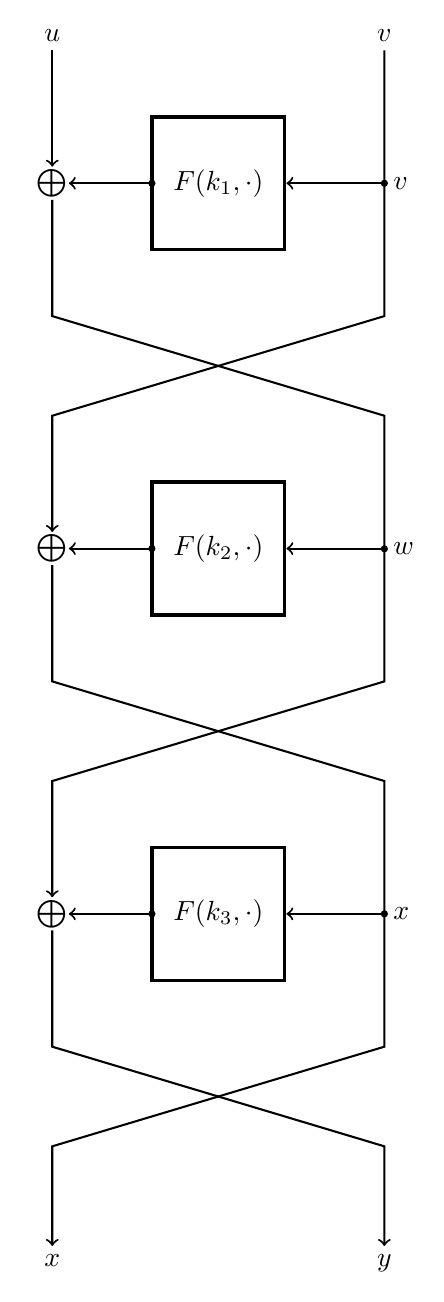
\begin{tikzpicture}[x=0.75pt,y=0.75pt,yscale=-0.8,xscale=0.8]


\draw  [line width=1.2]  (80,80) -- (160,80) -- (160,160) -- (80,160) -- cycle ;
\draw  [line width=1.2]  (80,300) -- (160,300) -- (160,380) -- (80,380) -- cycle ;
\draw  [line width=1.2]  (80,520) -- (160,520) -- (160,600) -- (80,600) -- cycle ;

\draw  [->]  (20,40) -- (20,110) ;
\draw  [->]  (20,130) -- (20,200) -- (220,260) -- (220,420) -- (20,480) -- (20,550) ;
\draw  [->]  (20,570) -- (20,640) -- (220,700) -- (220,760) ;
\draw  [->]  (220,40) -- (220,200) -- (20,260) -- (20,330) ;
\draw  [->]  (20,350) -- (20,420) -- (220,480) -- (220,640) -- (20,700) -- (20,760) ;

\draw  [->]  (80,120) -- (30,120) ;
\draw  [->]  (220,120) -- (161,120) ;
\draw  [->]  (80,340) -- (30,340) ;
\draw  [->]  (220,340) -- (161,340) ;
\draw  [->]  (80,560) -- (30,560) ;
\draw  [->]  (220,560) -- (161,560) ;

\draw  [fill={rgb, 255:red, 0; green, 0; blue, 0 }  ,fill opacity=1 ] (218.5,120) .. controls (218.5,119.17) and (219.17,118.5) .. (220,118.5) .. controls (220.83,118.5) and (221.5,119.17) .. (221.5,120) .. controls (221.5,120.83) and (220.83,121.5) .. (220,121.5) .. controls (219.17,121.5) and (218.5,120.83) .. (218.5,120) -- cycle ;
\draw  [fill={rgb, 255:red, 0; green, 0; blue, 0 }  ,fill opacity=1 ] (78.5,120) .. controls (78.5,119.17) and (79.17,118.5) .. (80,118.5) .. controls (80.83,118.5) and (81.5,119.17) .. (81.5,120) .. controls (81.5,120.83) and (80.83,121.5) .. (80,121.5) .. controls (79.17,121.5) and (78.5,120.83) .. (78.5,120) -- cycle ;
\draw  [fill={rgb, 255:red, 0; green, 0; blue, 0 }  ,fill opacity=1 ] (78.5,340) .. controls (78.5,339.17) and (79.17,338.5) .. (80,338.5) .. controls (80.83,338.5) and (81.5,339.17) .. (81.5,340) .. controls (81.5,340.83) and (80.83,341.5) .. (80,341.5) .. controls (79.17,341.5) and (78.5,340.83) .. (78.5,340) -- cycle ;
\draw  [fill={rgb, 255:red, 0; green, 0; blue, 0 }  ,fill opacity=1 ] (218.5,340.15) .. controls (218.5,339.33) and (219.17,338.65) .. (220,338.65) .. controls (220.83,338.65) and (221.5,339.33) .. (221.5,340.15) .. controls (221.5,340.98) and (220.83,341.65) .. (220,341.65) .. controls (219.17,341.65) and (218.5,340.98) .. (218.5,340.15) -- cycle ;
\draw  [fill={rgb, 255:red, 0; green, 0; blue, 0 }  ,fill opacity=1 ] (218.5,560) .. controls (218.5,559.17) and (219.17,558.5) .. (220,558.5) .. controls (220.83,558.5) and (221.5,559.17) .. (221.5,560) .. controls (221.5,560.83) and (220.83,561.5) .. (220,561.5) .. controls (219.17,561.5) and (218.5,560.83) .. (218.5,560) -- cycle ;
\draw  [fill={rgb, 255:red, 0; green, 0; blue, 0 }  ,fill opacity=1 ] (78.5,560) .. controls (78.5,559.17) and (79.17,558.5) .. (80,558.5) .. controls (80.83,558.5) and (81.5,559.17) .. (81.5,560) .. controls (81.5,560.83) and (80.83,561.5) .. (80,561.5) .. controls (79.17,561.5) and (78.5,560.83) .. (78.5,560) -- cycle ;

\draw (20,120) node  [font=\large]  {$\bigoplus $};
\draw (20,340) node  [font=\large]  {$\bigoplus $};
\draw (20,560) node  [font=\large]  {$\bigoplus $};
\draw (120,120) node    {$F( k_{1} ,\cdot )$};
\draw (120,340) node    {$F( k_{2} ,\cdot )$};
\draw (120,560) node    {$F( k_{3} ,\cdot )$};
\draw (20,36.6) node [anchor=south] [inner sep=0.75pt]    {$u$};
\draw (220,36.6) node [anchor=south] [inner sep=0.75pt]    {$v$};
\draw (223.5,120) node [anchor=west] [inner sep=0.75pt]    {$v$};
\draw (223.5,340.15) node [anchor=west] [inner sep=0.75pt]    {$w$};
\draw (223.5,560) node [anchor=west] [inner sep=0.75pt]    {$x$};
\draw (20,763.4) node [anchor=north] [inner sep=0.75pt]    {$x$};
\draw (220,763.4) node [anchor=north] [inner sep=0.75pt]    {$y$};


\end{tikzpicture}}
  \quad\quad\quad\quad
  \subfigure[解密]{

\tikzset{every picture/.style={line width=0.75pt}} %set default line width to 0.75pt        

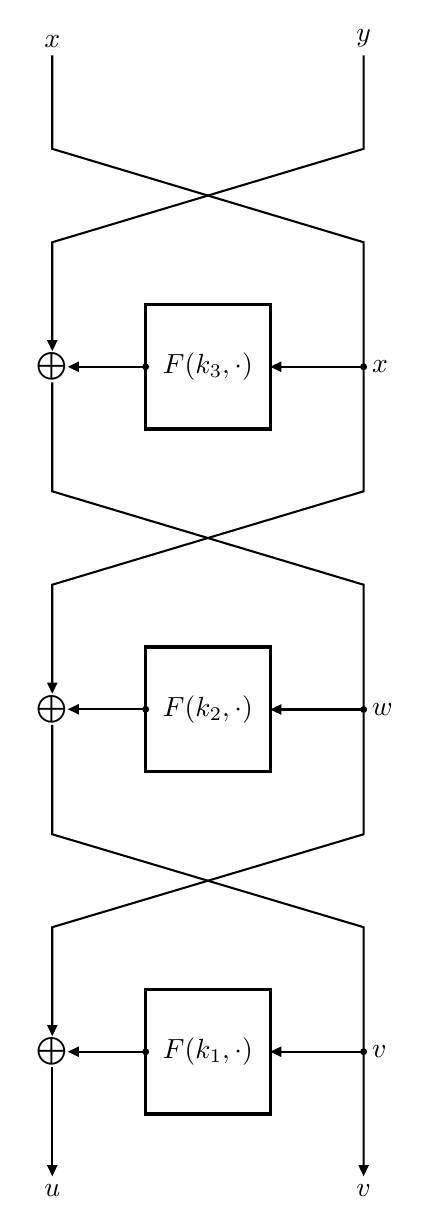
\begin{tikzpicture}[x=0.75pt,y=0.75pt,yscale=-0.75,xscale=0.75]
%uncomment if require: \path (0,809); %set diagram left start at 0, and has height of 809

%Shape: Rectangle [id:dp08810068320716669] 
\draw  [line width=1.2]  (80,200) -- (160,200) -- (160,280) -- (80,280) -- cycle ;
%Straight Lines [id:da7148920386750357] 
\draw    (20,249.96) -- (20,320) -- (220,380) -- (220,540.31) -- (20,600) -- (20,667) ;
\draw [shift={(20,670)}, rotate = 270] [fill={rgb, 255:red, 0; green, 0; blue, 0 }  ][line width=0.08]  [draw opacity=0] (7.14,-3.43) -- (0,0) -- (7.14,3.43) -- cycle    ;
%Shape: Rectangle [id:dp05753096156132376] 
\draw  [line width=1.2]  (80,420) -- (160,420) -- (160,500) -- (80,500) -- cycle ;
%Shape: Rectangle [id:dp5426589489554612] 
\draw  [line width=1.2]  (80,640) -- (160,640) -- (160,720) -- (80,720) -- cycle ;
%Straight Lines [id:da36785755794381103] 
\draw    (20,40) -- (20,100) -- (220,160) -- (220,320) -- (20,380) -- (20,447) ;
\draw [shift={(20,450)}, rotate = 270] [fill={rgb, 255:red, 0; green, 0; blue, 0 }  ][line width=0.08]  [draw opacity=0] (7.14,-3.43) -- (0,0) -- (7.14,3.43) -- cycle    ;
%Straight Lines [id:da5270839120181066] 
\draw    (220,40) -- (220,100) -- (20,160) -- (20,227) ;
\draw [shift={(20,230)}, rotate = 270] [fill={rgb, 255:red, 0; green, 0; blue, 0 }  ][line width=0.08]  [draw opacity=0] (7.14,-3.43) -- (0,0) -- (7.14,3.43) -- cycle    ;
%Straight Lines [id:da30154795477439555] 
\draw    (20,690) -- (20,757) ;
\draw [shift={(20,760)}, rotate = 270] [fill={rgb, 255:red, 0; green, 0; blue, 0 }  ][line width=0.08]  [draw opacity=0] (7.14,-3.43) -- (0,0) -- (7.14,3.43) -- cycle    ;
%Straight Lines [id:da9103919429832117] 
\draw    (20,470) -- (20,540.31) -- (220,600) -- (220,757) ;
\draw [shift={(220,760)}, rotate = 270] [fill={rgb, 255:red, 0; green, 0; blue, 0 }  ][line width=0.08]  [draw opacity=0] (7.14,-3.43) -- (0,0) -- (7.14,3.43) -- cycle    ;
%Straight Lines [id:da3209792329411032] 
\draw    (220,240) -- (163,240) ;
\draw [shift={(160,240)}, rotate = 360] [fill={rgb, 255:red, 0; green, 0; blue, 0 }  ][line width=0.08]  [draw opacity=0] (7.14,-3.43) -- (0,0) -- (7.14,3.43) -- cycle    ;
%Straight Lines [id:da07595236987438247] 
\draw    (80,240) -- (33,240) ;
\draw [shift={(30,240)}, rotate = 360] [fill={rgb, 255:red, 0; green, 0; blue, 0 }  ][line width=0.08]  [draw opacity=0] (7.14,-3.43) -- (0,0) -- (7.14,3.43) -- cycle    ;
%Straight Lines [id:da8515371795008031] 
\draw    (220,460.15) -- (163,460.15) ;
\draw [shift={(160,460.15)}, rotate = 360] [fill={rgb, 255:red, 0; green, 0; blue, 0 }  ][line width=0.08]  [draw opacity=0] (7.14,-3.43) -- (0,0) -- (7.14,3.43) -- cycle    ;
%Straight Lines [id:da08233223837321657] 
\draw    (220,680) -- (163,680) ;
\draw [shift={(160,680)}, rotate = 360] [fill={rgb, 255:red, 0; green, 0; blue, 0 }  ][line width=0.08]  [draw opacity=0] (7.14,-3.43) -- (0,0) -- (7.14,3.43) -- cycle    ;
%Straight Lines [id:da3216064715402762] 
\draw    (80,460) -- (33,460) ;
\draw [shift={(30,460)}, rotate = 360] [fill={rgb, 255:red, 0; green, 0; blue, 0 }  ][line width=0.08]  [draw opacity=0] (7.14,-3.43) -- (0,0) -- (7.14,3.43) -- cycle    ;
%Straight Lines [id:da0911188498517359] 
\draw    (80,680) -- (33,680) ;
\draw [shift={(30,680)}, rotate = 360] [fill={rgb, 255:red, 0; green, 0; blue, 0 }  ][line width=0.08]  [draw opacity=0] (7.14,-3.43) -- (0,0) -- (7.14,3.43) -- cycle    ;
%Shape: Circle [id:dp5566373818887096] 
\draw  [fill={rgb, 255:red, 0; green, 0; blue, 0 }  ,fill opacity=1 ] (218.5,240) .. controls (218.5,239.17) and (219.17,238.5) .. (220,238.5) .. controls (220.83,238.5) and (221.5,239.17) .. (221.5,240) .. controls (221.5,240.83) and (220.83,241.5) .. (220,241.5) .. controls (219.17,241.5) and (218.5,240.83) .. (218.5,240) -- cycle ;
%Shape: Circle [id:dp14089569320942252] 
\draw  [fill={rgb, 255:red, 0; green, 0; blue, 0 }  ,fill opacity=1 ] (78.5,240) .. controls (78.5,239.17) and (79.17,238.5) .. (80,238.5) .. controls (80.83,238.5) and (81.5,239.17) .. (81.5,240) .. controls (81.5,240.83) and (80.83,241.5) .. (80,241.5) .. controls (79.17,241.5) and (78.5,240.83) .. (78.5,240) -- cycle ;
%Shape: Circle [id:dp9889295507534646] 
\draw  [fill={rgb, 255:red, 0; green, 0; blue, 0 }  ,fill opacity=1 ] (78.5,460) .. controls (78.5,459.17) and (79.17,458.5) .. (80,458.5) .. controls (80.83,458.5) and (81.5,459.17) .. (81.5,460) .. controls (81.5,460.83) and (80.83,461.5) .. (80,461.5) .. controls (79.17,461.5) and (78.5,460.83) .. (78.5,460) -- cycle ;
%Shape: Circle [id:dp6544997090075493] 
\draw  [fill={rgb, 255:red, 0; green, 0; blue, 0 }  ,fill opacity=1 ] (218.5,460.15) .. controls (218.5,459.33) and (219.17,458.65) .. (220,458.65) .. controls (220.83,458.65) and (221.5,459.33) .. (221.5,460.15) .. controls (221.5,460.98) and (220.83,461.65) .. (220,461.65) .. controls (219.17,461.65) and (218.5,460.98) .. (218.5,460.15) -- cycle ;
%Shape: Circle [id:dp16907136977415704] 
\draw  [fill={rgb, 255:red, 0; green, 0; blue, 0 }  ,fill opacity=1 ] (218.5,680) .. controls (218.5,679.17) and (219.17,678.5) .. (220,678.5) .. controls (220.83,678.5) and (221.5,679.17) .. (221.5,680) .. controls (221.5,680.83) and (220.83,681.5) .. (220,681.5) .. controls (219.17,681.5) and (218.5,680.83) .. (218.5,680) -- cycle ;
%Shape: Circle [id:dp3827346476021749] 
\draw  [fill={rgb, 255:red, 0; green, 0; blue, 0 }  ,fill opacity=1 ] (78.5,680) .. controls (78.5,679.17) and (79.17,678.5) .. (80,678.5) .. controls (80.83,678.5) and (81.5,679.17) .. (81.5,680) .. controls (81.5,680.83) and (80.83,681.5) .. (80,681.5) .. controls (79.17,681.5) and (78.5,680.83) .. (78.5,680) -- cycle ;

% Text Node
\draw (20,240) node   {$\bigoplus $};
% Text Node
\draw (20,460) node   {$\bigoplus $};
% Text Node
\draw (20,680) node   {$\bigoplus $};
% Text Node
\draw (120,240) node    {$F( k_{3} ,\cdot )$};
% Text Node
\draw (120,460) node    {$F( k_{2} ,\cdot )$};
% Text Node
\draw (120,680) node    {$F( k_{1} ,\cdot )$};
% Text Node
\draw (20,36.6) node [anchor=south] [inner sep=0.75pt]    {$x$};
% Text Node
\draw (220,36.6) node [anchor=south] [inner sep=0.75pt]    {$y$};
% Text Node
\draw (223.5,240) node [anchor=west] [inner sep=0.75pt]    {$x$};
% Text Node
\draw (223.5,460.15) node [anchor=west] [inner sep=0.75pt]    {$w$};
% Text Node
\draw (223.5,680) node [anchor=west] [inner sep=0.75pt]    {$v$};
% Text Node
\draw (220,763.4) node [anchor=north] [inner sep=0.75pt]    {$v$};
% Text Node
\draw (20,763.4) node [anchor=north] [inner sep=0.75pt]    {$u$};


\end{tikzpicture}}
  \caption{使用卢比-拉克福构造进行加密和解密}
  \label{fig:4-14}
\end{figure}

容易看出,$\mathcal{E}$ 是一个分组密码。可以认为算法 $E$ 由三``轮"运算组成。对于 $k\in\mathcal{K}$,我们定义``轮函数"为:
\[
\begin{aligned}
\phi_k:\quad\mathcal{X}^2 & \to \mathcal{X}^2\\
(a,b) & \mapsto (b,a\oplus F(k,b))
\end{aligned}
\]

不难看出,对于任意固定的 $k$,函数 $\phi_k$ 都是 $\mathcal{X}^2$ 上的一个置换。事实上,如果令 $\sigma(a,b):=(b,a)$,则有:
\[
\phi_k^{-1}=\sigma\circ\phi_k\circ\sigma
\]
此外,我们可以发现:
\[
E((k_1,k_2,k_3),\cdot)=\phi_{k_3}\circ\phi_{k_2}\circ\phi_{k_1} 
\]
和:
\[
D((k_1,k_2,k_3),\cdot)=\phi^{-1}_{k_1}\circ\phi^{-1}_{k_2}\circ\phi^{-1}_{k_3}=\sigma\circ\phi_{k_1}\circ\phi_{k_2}\circ\phi_{k_3}\circ\sigma
\]

\begin{theorem}
如果 $F$ 是一个安全 PRF,且 $N:=|\mathcal{X}|=2^n$ 是超多项式的,那么由 $F$ 构建的卢比-拉克福密码 $\mathcal{E}=(E,D)$ 是一个安全的分组密码。
\begin{quote}
特别地,对于每一个如攻击游戏 \ref{game:4-1} 中那样攻击 $\mathcal{E}$ 的 $Q$ 次查询BC对手 $\mathcal{A}$,都存在一个就 $F$ 进行攻击游戏 \ref{game:4-2} 的 PRF 对手 $\mathcal{B}$,其中 $\mathcal{B}$ 是一个围绕 $\mathcal{A}$ 的基本包装器,满足:
\end{quote}
\[
{\rm BC\mathsf{adv}}[\mathcal{A},\mathcal{E}]\leq3\cdot{\rm PRF\mathsf{adv}}[\mathcal{B},F]+\frac{Q^2}{N}+\frac{Q^2}{2N^2}
\]
\end{theorem}

\begin{proof}[证明思路]
根据推论 \ref{cor:4-5},由于我们假设 $N$ 是超多项式的,所以只需要证明 $\mathcal{E}$ 是一个安全 PRF 即可。因此,我们想要证明,如果对手在攻击游戏 \ref{game:4-2} 的实验 $0$ 中针对 $\mathcal{E}$ 进行游戏,挑战者的回应实际上``看起来像"完全随机的比特序列。我们可以假设对手永远不会发起两次相同的查询。此外,由于 $F$ 是一个 PRF,我们可以用真随机函数 $f_1$,$f_2$ 和 $f_3$ 来代替伪随机函数 $F(k_1,\cdot)$,$F(k_2,\cdot)$ 和 $F(k_3,\cdot)$,而对手应该很难注意到这种区别。

因此,现在给定一个查询 $(u_i,v_i)$,挑战者按如下方式计算应答 $(x_i,y_i)$:

\vspace{5pt}

\hspace*{5pt} $w_i\leftarrow u_i\oplus f_1(v_i)$\\
\hspace*{26pt} $x_i\leftarrow v_i\oplus f_2(w_i)$\\
\hspace*{26pt} $y_i\leftarrow w_i\oplus f_3(x_i)$

\vspace{5pt}

一个粗略、直观的论证是这样的。假设没有任何两个 $w_i$ 值是相同的,那么 $f_2$ 的所有输出都是随机且相互独立的。由此,我们可以论证 $x_i$ 也是随机且相互独立的。因此 $f_3$ 的输入存在相同值的概率可忽略不计。由此,我们可以得出结论,$y_i$ 们基本上都是随机且相互独立的。

因此,如果我们能证明所有的 $w_i$ 都是不同的,情况就会很好。而 $w_i$ 是由随机函数 $f_1$ 间接得到的,所以只要小心一点,确实可以论证 $w_i$ 中存在相同值的概率可忽略不计。
\end{proof}

\begin{proof}
假设 $\mathcal{A}$ 是一个有效BC对手,它对 $\mathcal{E}$ 进行攻击游戏 \ref{game:4-1} 中的攻击,并且对挑战者发起最多 $Q$ 次查询。我们想证明 ${\rm BC\mathsf{adv}}[\mathcal{A},\mathcal{E}]$ 可忽略不计。要做到这一点,我们首先要证明 ${\rm PRF\mathsf{adv}}[\mathcal{A}, E]$ 是可忽略不计的,然后基于 PRF 切换引理(即定理 \ref{theo:4-4})和 $N$ 是超多项式的假设中得出结果。

简便起见,我们用一个具备以下特性的对手 $\mathcal{A}_0$ 来代替 $\mathcal{A}$:
\begin{itemize}
	\item $\mathcal{A}_0$ 总是对其挑战者进行恰好 $Q$ 次查询;
	\item $\mathcal{A}_0$ 不会多次进行相同的查询;
	\item $\mathcal{A}_0$ 和 $\mathcal{A}$ 一样有效(更确切地说,$\mathcal{A}_0$ 是一个围绕 $\mathcal{A}$ 的基本包装器);
	\item ${\rm PRF\mathsf{adv}}[\mathcal{A}_0, E]={\rm PRF\mathsf{adv}}[\mathcal{A}, E]$。
\end{itemize}
对手 $\mathcal{A}_0$ 只是简单地运行与$\mathcal{A}$相同的协议;然而,它保留了一张查询/应答表,以避免重复查询;此外,如有必要,$\mathcal{A}_0$ 会``填充" $\mathcal{A}$ 的执行次数,以确保发起查询的次数正好是 $Q$。

该证明的总体策略如下。首先,我们将游戏 $0$ 定义为 $\mathcal{A}_0$ 与攻击游戏 \ref{game:4-2} 的实验 $0$ 的挑战者之间就 $E$ 进行的游戏。然后,我们再定义几个游戏:游戏 $1$,游戏 $2$ 和游戏 $3$。每一个游戏都是在 $\mathcal{A}_0$ 和不同的挑战者之间进行的;此外,游戏 $3$ 中的挑战者等同于攻击游戏 \ref{game:4-2} 的实验 $1$ 的挑战者。另外,对于 $j=0,\dots,3$,我们定义 $W_j$ 为 $\mathcal{A}_0$ 在游戏 $j$ 中输出 $1$ 的事件。我们将表明,对于 $j=1,\dots,3$,$|\Pr[W_j]-\Pr[W_{j-1}]|$ 的值可忽略不计,由此,我们可以得到:
\[
|\Pr[W_3]-\Pr[W_0]|={\rm PRF\mathsf{adv}}[\mathcal{A}_0, E]
\]
也是可忽略不计的。

\vspace{5pt}

\noindent
\textbf{游戏 $\mathbf{0}$}。
我们首先详细描述游戏 $0$ 中的挑战者:

\vspace{5pt}

\hspace*{5pt} 选取 $k_1,k_2,k_3\overset{\rm R}\leftarrow\mathcal{K}$\\
\hspace*{26pt} 当收到第 $i$ 个查询 $(u_i,v_i)\in\mathcal{X}^2\;\;(i=1,\dots,Q)$ 时,计算:\\
\hspace*{50pt} $w_i\leftarrow u_i\oplus F(k_1,v_i)$\\
\hspace*{50pt} $x_i\leftarrow v_i\oplus F(k_2,w_i)$\\
\hspace*{50pt} $y_i\leftarrow w_i\oplus F(k_3,x_i)$\\
\hspace*{50pt} 将 $(x_i,y_i)$ 发送给对手。

\vspace{5pt}

\noindent
回顾一下,对手 $\mathcal{A}_0$ 保证总是会发起 $Q$ 次不同的查询 $(u_1,v_1),\dots,(u_Q,v_Q)$;也就是说,$(u_i,v_i)$ \emph{作为数对}是各不相同的;所以对于 $i\neq j$,我们可能有 $u_i=u_j$ 或 $v_i=v_j$,但是两者不能同时成立。

\vspace{5pt}

\noindent
\textbf{游戏 $\mathbf{1}$}。
我们接下来打``PRF牌",即用真随机函数 $f_1$,$f_2$ 和 $f_3$ 来代替三个伪随机函数 $F(k_1,\cdot)$,$F(k_2,\cdot)$ 和 $F(k_3,\cdot)$。因此,我们在游戏 $1$ 中的挑战者运行如下:

\vspace{5pt}

\hspace*{5pt} 选取 $f_1,f_2,f_3\overset{\rm R}\leftarrow{\rm Funs}[\mathcal{X},\mathcal{X}]$\\
\hspace*{26pt} 当收到第 $i$ 个查询 $(u_i,v_i)\in\mathcal{X}^2\;\;(i=1,\dots,Q)$ 时,计算:\\
\hspace*{50pt} $w_i\leftarrow u_i\oplus f_1(v_i)$\\
\hspace*{50pt} $x_i\leftarrow v_i\oplus f_2(w_i)$\\
\hspace*{50pt} $y_i\leftarrow w_i\oplus f_3(x_i)$\\
\hspace*{50pt} 将 $(x_i,y_i)$ 发送给对手。

\vspace{5pt}

如练习 4.26 中将要讨论的,我们可以将三个伪随机函数 $F(k_1,\cdot)$,$F(k_2,\cdot)$ 和 $F(k_3,\cdot)$ 建模为一个单一的 PRF $F'$,称其为 $F$ 的 $3$ 次并行组合:PRF $F'$ 定义在 $(\mathcal{K}^3,\{1,2,3\}\times\mathcal{X},\mathcal{X})$ 上,且 $F'((k_1,k_2,k_3),(s,x)):=F(k_s,x)$。我们很容易构造一个和 $\mathcal{A}_0$ 一样有效的对手 $\mathcal{B}'$,使得:
\begin{equation}\label{eq:4-24}
|\Pr[W_1]-\Pr[W_0]|={\rm PRF\mathsf{adv}}[\mathcal{B}', F']
\end{equation}
对手 $\mathcal{B}'$ 简单地运行 $\mathcal{A}_0$,并原样输出 $\mathcal{A}_0$ 所输出的任何东西。当 $\mathcal{A}_0$ 用一个数对 $(u_i,v_i)$ 查询其挑战者时,对手 $\mathcal{B}'$ 通过计算:

\vspace{5pt}

\hspace*{5pt} $w_i\leftarrow u_i\oplus f'(1,v_i)$\\
\hspace*{26pt} $x_i\leftarrow v_i\oplus f'(2,w_i)$\\
\hspace*{26pt} $y_i\leftarrow w_i\oplus f'(3,x_i)$

\vspace{5pt}

\noindent
来得到要交给 $\mathcal{A}_0$ 的应答 $(x_i,y_i)$。这里,$f'$ 表示 $\mathcal{B}'$ 的挑战者在攻击游戏 \ref{game:4-2} 中就 $F'$ 所选择的函数。很明显,$\mathcal{B}'$ 在该攻击游戏的实验 $0$ 中以概率 $\Pr[W_0]$ 输出 $1$,而在实验 $1$ 中以概率 $\Pr[W_1]$ 输出 $1$,由此可得式 \ref{eq:4-24}。

根据练习 4.26,存在一个和 $\mathcal{B}'$ 一样有效的对手 $\mathcal{B}$,满足:
\begin{equation}\label{eq:4-25}
{\rm PRF\mathsf{adv}}[\mathcal{B}', F']= 3\cdot {\rm PRF\mathsf{adv}}[\mathcal{B}, F]
\end{equation}

\noindent
\textbf{游戏 $\mathbf{2}$}。
接下来我们做一个纯粹的概念上的改变:我们用 \ref{subsec:4-4-2} 小节中讨论的``忠实的侏儒"来实现随机函数 $f_2$ 和 $f_3$。这样做并不是为了提高效率,而是为了给我们做准备,以便之后在游戏 $3$ 中能够做出更实质性(也更易分析)的修改。我们在这个游戏中的挑战者的工作方式如下:

\vspace{5pt}

\hspace*{5pt} 选取 $f_1\overset{\rm R}\leftarrow{\rm Funs}[\mathcal{X},\mathcal{X}]$\\
\hspace*{26pt} 选取 $X_1,\dots,X_Q\overset{\rm R}\leftarrow\mathcal{X}$\\
\hspace*{26pt} 选取 $Y_1,\dots,Y_Q\overset{\rm R}\leftarrow\mathcal{X}$\\
\hspace*{26pt} 当收到第 $i$ 个查询 $(u_i,v_i)\in\mathcal{X}^2\;\;(i=1,\dots,Q)$ 时:\\
\hspace*{50pt} 计算 $w_i\leftarrow u_i\oplus f_1(v_i)$\\
\hspace*{50pt} 令 $x_i'\leftarrow X_i$;
				\framebox[\width]{~如果存在 $j<i$ 使得 $w_i=w_j$,则令 $x_i'\leftarrow x_j'$;}
				令 $x_i\leftarrow v_i\oplus x_i'$\\
\hspace*{50pt} 令 $y_i'\leftarrow Y_i$;
				\framebox[\width]{~如果存在 $j<i$ 使得 $x_i=x_j$,则令 $y_i'\leftarrow y_j'$;}
				令 $y_i\leftarrow w_i\oplus y_i'$\\
\hspace*{50pt} 将 $(x_i,y_i)$ 发送给对手。

\vspace{5pt}

\noindent
这个的想法是,$x_i'$ 的值代表 $f_2(w_i)$。默认情况下,$x_i'$ 等于随机值 $X_i$;然而,如果存在某个 $j<i$ 使得 $w_i=w_j$,上面被框住的逻辑就会覆写这个默认值。同样地,$y_i'$ 的值代表 $f_3(x_i)$。在默认情况下,$y_i'$ 等于随机值 $Y_i$,但如有必要,框住的逻辑就会覆写默认值。

由于游戏 $2$ 中的挑战者完全等同于游戏 $1$ 中的挑战者,我们有:
\begin{equation}\label{eq:4-26}
\Pr[W_2]=Pr[W_1]
\end{equation}

\noindent
\textbf{游戏 $\mathbf{3}$}。
我们现在采用``健忘的侏儒"技术,如之前在定理 \ref{theo:4-6} 的证明中介绍的那样。我们的想法是简单地消除挑战者在游戏 $2$ 中进行的的重复检查。挑战者在游戏 $3$ 中的运行流程如下:

\vspace{5pt}

\hspace*{5pt} 选取 $f_1\overset{\rm R}\leftarrow{\rm Funs}[\mathcal{X},\mathcal{X}]$\\
\hspace*{26pt} 选取 $X_1,\dots,X_Q\overset{\rm R}\leftarrow\mathcal{X}$\\
\hspace*{26pt} 选取 $Y_1,\dots,Y_Q\overset{\rm R}\leftarrow\mathcal{X}$\\
\hspace*{26pt} 当收到第 $i$ 个查询 $(u_i,v_i)\in\mathcal{X}^2\;\;(i=1,\dots,Q)$ 时:\\
\hspace*{50pt} 计算 $w_i\leftarrow u_i\oplus f_1(v_i)$\\
\hspace*{50pt} 令 $x_i'\leftarrow X_i$;令 $x_i\leftarrow v_i\oplus x_i'$\\
\hspace*{50pt} 令 $y_i'\leftarrow Y_i$;令 $y_i\leftarrow w_i\oplus y_i'$\\
\hspace*{50pt} 将 $(x_i,y_i)$ 发送给对手。

\vspace{5pt}

请注意,这一描述与游戏 $2$ 中对挑战者的描述完全相同,我们只是简单地抹去了后者中被框住的逻辑。

为了分析,我们把游戏 $2$ 和游戏 $3$ 看作是运行在相同的基础概率空间上。这个概率空间是取决于以下因素:
\begin{itemize}
	\item 对手所做的随机选择,我们用 $Coins$ 表示,以及
	\item 挑战者所做的随机选择,即 $f_1,X_1,\dots,X_Q$ 和 $Y_1,\dots,Y_Q$。
\end{itemize}
这两个游戏间的不同之处在于挑战者针对对手查询给出应答的策略。

\vspace{5pt}

\noindent
\textbf{声称$\mathbf{1}$:}
\emph{在游戏 3 中,随机变量 $Coins,f_1,x_1,y_1,\dots,x_Q,y_Q$ 是相互独立的。}为了证明这一声称,根据构造,随机变量:
\[
Coins,\quad
f_1,\quad
X_1,\dots,X_Q,\quad
Y_1,\dots,Y_Q
\]
是相互独立的。现在以 $Coins$ 和 $f_1$ 的任何固定值为条件。第一个查询 $(u_1,v_1)$ 现在是固定的,因此 $w_1$ 也是固定的;然而,在这个条件概率空间中,$X_1$ 和 $Y_1$ 仍然在 $\mathcal{X}$ 上均匀独立分布,因此 $x_1$ 和 $y_1$ 也是均匀且独立分布的。我们继续论证,以 $x_1,y_1$ 的固定值为条件(除了 $Coins$ 和 $f_1$ 的固定值之外),观察到现在 $u_2$,$v_2$ 和 $w_2$ 也是固定的,并且 $x_2$ 和 $y_2$ 是均匀独立分布的。我们应该可以清楚的看到,通过归纳法就可以证明声称 $1$ 成立。

令 $Z_1$ 表示在游戏 $3$ 中存在某个 $i\neq j$ 使得 $w_i=w_j$ 成立的事件,$Z_2$ 表示在游戏 $3$ 中存在某个 $i\neq j$ 使得 $x_i=x_j$ 成立的事件,令 $Z:=Z_1\lor Z_2$。请注意,事件 $Z$ 的定义基于游戏 $3$ 中变量 $w_i$ 和 $x_i$ 的取值。事实上,变量 $w_i$ 和 $z_i$ 在游戏 $2$ 和游戏 $3$ 中的计算方式可能不一样,所以我们在游戏 $3$ 中显式地用它们的值来定义事件 $Z$。尽管如此,我们可以直接看到,如果 $Z$ 没有发生,游戏 $2$ 和游戏 $3$ 的进程是相同的。特别是:

\vspace{5pt}

\noindent
\textbf{声称$\mathbf{2}$:}
\emph{当且仅当事件 $W_3\land\bar Z$ 发生时,事件 $W_2\land\bar Z$ 发生。}为了证明该声称,考虑事件 $Z$ 不发生的情况下,变量:
\[
Coins,\quad
f_1,\quad
X_1,\dots,X_Q,\quad
Y_1,\dots,Y_Q
\]
的任何固定值。只要说明 $\mathcal{A}_0$ 的输出在游戏 $2$ 和游戏 $3$ 中都是一样的就足够了。由于查询 $(u_1,v_1)$ 只取决于 $Coins$,我们可以看到变量 $u_1,v_1$,以及 $w_1,x_1,y_1$ 在两个游戏中都有相同的值。由于查询 $(u_2,v_2)$ 只取决于 $Coins$ 和 $(x_1,y_1)$,因此变量 $u_2,v_2$ 以及 $w_2$ 在两个游戏中都有相同的值;而由于 $Z$ 未发生,我们可知 $w_2\neq w_1$,因此变量 $x_2$ 在两个游戏中都有相同的值;同样,由于 $Z$ 未发生,因此有 $x_2\neq x_1$,所以变量 $y_2$ 在两个游戏中有相同值。以此类推,我们可以看到对于 $i=1,\dots,Q$,变量 $u_i,v_i,w_i,x_i,y_i$ 在两个游戏中都有相同值。由于 $\mathcal{A}_0$ 的输出是这些变量和 $Coins$ 的函数,所以它在两个游戏中的输出也是相同的。因此声称 $2$ 得证。

声称 $2$,连同差分引理(即定理 \ref{theo:4-7})和联合约束可以导出:
\begin{equation}\label{eq:4-27}
|\Pr[W_3]-\Pr[W_2]|\leq\Pr[Z]\leq\Pr[Z_1]+\Pr[Z_2]
\end{equation}

由于 $x_1,\dots,x_Q$ 是相互独立的(见声称$1$),显然有:
\begin{equation}\label{eq:4-28}
\Pr[Z_2]\leq\frac{Q^2}{2}\cdot\frac{1}{N}
\end{equation}
因为 $Z_2$ 是少于 ${Q^2}/{2}$ 个事件的联合,其中每个事件发生的概率为 ${1}/{N}$。

下面我们分析事件 $Z_1$。我们声称:
\begin{equation}\label{eq:4-29}
\Pr[Z_1]\leq\frac{Q^2}{2}\cdot\frac{1}{N}
\end{equation}
为了证明这一点,只需证明它是以 $Coins,x_1,y_1,\dots,x_Q,y_Q$ 的任何固定值为条件。如果这些值是固定的,那么 $u_1,v_1,\dots,u_Q,v_Q$ 也是固定的。然而,根据独立性(见声称 $1$),变量 $f_1$ 在这个条件概率空间的 ${\rm Funs}[\mathcal{X},\mathcal{X}]$ 上仍然是均匀分布的。现在,考虑任何一对固定索引 $i,j$,其中 $i\neq j$。首先假设 $v_i=v_j$,那么,由于 $\mathcal{A}_0$ 从来不会发起两次相同的查询,我们必有 $u_i\neq u_j$,而且很容易看到,对于任何 $f_1$ 的选择,都有 $w_i\neq w_j$。接下来,假设 $v_i\neq v_j$,那么 $f_1(v_i)$ 和 $f_1(v_j)$ 的值在这个条件概率空间的 $\mathcal{X}$ 上是均匀独立分布的,且在该条件概率空间上有:
\[
\Pr[f_1(v_i)\oplus f_1(v_j)=u_i\oplus u_j]=\frac{1}{N}
\]

因此,我们证明了在游戏 $3$ 中,对于任意满足 $i\neq j$ 的索引对 $i,j$,有:
\[
\Pr[w_i=w_j]\leq\frac{1}{N}
\]
那么由联合约束,就可以得到式 \ref{eq:4-29}。

作为声称 $1$ 的另一个结论,我们观察到,就 $\mathcal{E}$ 而言,游戏 $3$ 等同于攻击游戏 \ref{game:4-2} 的实验 $1$。由此,连同式 \ref{eq:4-24},\ref{eq:4-25},\ref{eq:4-26},\ref{eq:4-27},\ref{eq:4-28} 和\ref{eq:4-29},我们可以得到以下结论:
\[
{\rm PRF\mathsf{adv}}[\mathcal{A}_0,E]\leq3\cdot{\rm PRF\mathsf{adv}}[\mathcal{B},F]+\frac{Q^2}{N}
\]
最后,将定理 \ref{theo:4-4} 应用于数据分组空间大小为 $N^2$ 的密码 $\mathcal{E}$,我们就有:
\[
{\rm BC\mathsf{adv}}[\mathcal{A},\mathcal{E}]\leq3\cdot{\rm PRF\mathsf{adv}}[\mathcal{B},F]+\frac{Q^2}{N}+\frac{Q^2}{2N^2}
\]
于是该定理得证。
\end{proof}
\section{树构造:从 PRG 到 PRF}\label{sec:4-6}

事实证明,给定一个合适的、安全的 PRG,我们可以用一种叫做\textbf{树构造 (tree construction)}的技术来构建一个安全的 PRF。将这一结果与 \ref{sec:4-5} 节中的卢比-拉克福构造相结合,我们可以看到,我们可以基于任何一个安全 PRG 构造出一个安全的分组密码。虽然这一结果具有一定的理论意义,但这种构造并不十分高效,而且在实践中也没有被真正使用。然而,我们注意到,这种构造的一种简单推广在实际的消息认证方案中发挥着重要的作用,我们将在 \ref{subsec:6-4-2} 小节中讨论这个问题。

我们从一个定义在 $(\mathcal{S},\mathcal{S}^2)$ 上的伪随机数生成器 $G$ 开始。也就是说,$G$ 的种子空间是一个集合 $\mathcal{S}$,而输出空间是所有种子对的集合 $\mathcal{S}^2$。比如,$G$ 可以将 $n$ 比特序列拉伸为 $2n$ 比特的序列\footnote[2]{事实上,我们甚至可以从一个 PRG 开始,将 $n$ 比特的序列拉伸为 $(n+1)$ 比特,然后应用定理 \ref{theo:3-3} 中分析的$n$次串行组合构造来获得一个合适的 $G$。}。方便的做法是将其表示成$G(s) = (G_0(s),G_1(s))$;也就是说,$G_0(s)\in\mathcal{S}$ 表示 $G(s)$ 的第一个组成部分,$G_1(s)$ 表示 $G(s)$ 的第二个组成部分。我们将基于 $G$ 构造一个伪随机函数 $F$,其密钥空间为 $\mathcal{S}$,输入空间为 $\{0,1\}^\ell$(其中 $\ell$ 是一个任意的、多项式边界的值),输出空间为 $\mathcal{S}$。

我们首先定义一个算法 $G^*$,它接受 $s\in\mathcal{S}$ 和 $x=(a_1,\dots,a_n)\in\{0,1\}^n$ 作为输入,其中对于 $i=1,\dots,n$ 有 $a_i\in\{0,1\}$,输出一个元素 $t\in\mathcal{S}$,其工作原理如下:

\vspace{5pt}

\hspace*{5pt} 令 $t\leftarrow s$\\
\hspace*{26pt} 对于 $i=1,\dots,n$:\\
\hspace*{50pt} 令 $t\leftarrow G_{a_i}(t)$\\
\hspace*{26pt} 输出 $t$。

\vspace{5pt}

\noindent
对于 $s\in\mathcal{S}$ 和 $x\in\{0,1\}^\ell$,我们定义:
\[
F(s,x):=G^*(s,x)
\]
我们将用这种方式从 $G$ 派生出来的 PRF $F$ 称为\textbf{树构造}。

不妨将输入 $x\in\{0,1\}^\ell$ 的各个比特想象成一棵高为 $\ell$,有 $2^\ell$ 个叶子结点的完全二叉树上的一条由根结点到叶子结点的追踪路径。我们将这棵树称为\textbf{评估树 (evaluation tree)},比特为 $0$ 意味着左子树,为 $1$ 则意味着右子树。这样一来,树中的任何结点都可以由一个长度最多为 $\ell$ 的比特序列唯一寻址;长度为 $j\leq\ell$ 的比特序列能够寻址到树中第 $j$ 层中的结点:空序列可以寻址到根结点(位于第$0$层),长度为 $1$ 的序列可以寻址到根结点的两个子结点(位于第$1$层),以此类推。评估树中的所有结点都可以使用以下规则,用 $\mathcal{S}$ 中的元素来标记:
\begin{itemize}
	\item 树根结点的标签为 $s$;
	\item 任何其他的结点都是由其父结点的标签$t$\textbf{派生}而来,方法如下:如果该结点是左子结点,则其标签为$G_0(t)$,如果该结点是右子结点,则其标签为$G_1(t)$。
\end{itemize}
那么 $F(s,x)$ 的值就对应由 $x$ 寻址的叶子结点的标签,如图 \ref{fig:4-15} 所示。

\begin{figure}
  \centering
  

\tikzset{every picture/.style={line width=0.75pt}} %set default line width to 0.75pt        

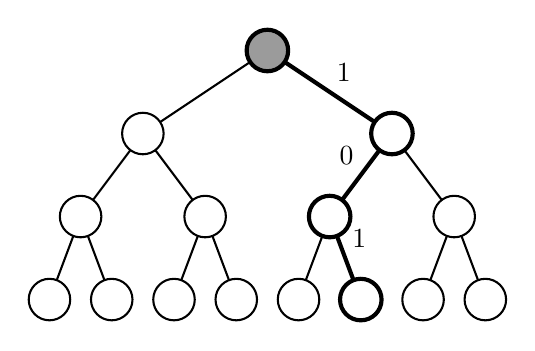
\begin{tikzpicture}[x=0.75pt,y=0.75pt,yscale=-1,xscale=1]
%uncomment if require: \path (0,201); %set diagram left start at 0, and has height of 201

%Straight Lines [id:da918933314477578] 
\draw    (25,90) -- (10,130) ;
%Straight Lines [id:da17752403794816818] 
\draw    (25,90) -- (40,130) ;
%Straight Lines [id:da39739380547431047] 
\draw    (85,90) -- (70,130) ;
%Straight Lines [id:da8176534439302041] 
\draw    (85,90) -- (100,130) ;
%Straight Lines [id:da11119551564082819] 
\draw    (145,90) -- (130,130) ;
%Straight Lines [id:da03948368488437359] 
\draw [line width=1.5]    (145,90) -- (160,130) ;
%Straight Lines [id:da6961629200987864] 
\draw    (205,90) -- (190,130) ;
%Straight Lines [id:da2074079789109078] 
\draw    (205,90) -- (220,130) ;
%Straight Lines [id:da5468814977357803] 
\draw    (55,50) -- (25,90) ;
%Straight Lines [id:da9893002745985011] 
\draw    (55,50) -- (85,90) ;
%Straight Lines [id:da8593115230517709] 
\draw [line width=1.5]    (175,50) -- (145,90) ;
%Straight Lines [id:da23020903575475726] 
\draw    (175,50) -- (205,90) ;
%Straight Lines [id:da03126695179086236] 
\draw    (115,10) -- (55,50) ;
%Straight Lines [id:da3788608056533551] 
\draw [line width=1.5]    (115,10) -- (175,50) ;
%Shape: Circle [id:dp7171076115795707] 
\draw  [fill={rgb, 255:red, 255; green, 255; blue, 255 }  ,fill opacity=1 ][line width=0.75]  (0,130) .. controls (0,124.48) and (4.48,120) .. (10,120) .. controls (15.52,120) and (20,124.48) .. (20,130) .. controls (20,135.52) and (15.52,140) .. (10,140) .. controls (4.48,140) and (0,135.52) .. (0,130) -- cycle ;
%Shape: Circle [id:dp9368220803834215] 
\draw  [fill={rgb, 255:red, 255; green, 255; blue, 255 }  ,fill opacity=1 ][line width=0.75]  (30,130) .. controls (30,124.48) and (34.48,120) .. (40,120) .. controls (45.52,120) and (50,124.48) .. (50,130) .. controls (50,135.52) and (45.52,140) .. (40,140) .. controls (34.48,140) and (30,135.52) .. (30,130) -- cycle ;
%Shape: Circle [id:dp48873250304858695] 
\draw  [fill={rgb, 255:red, 255; green, 255; blue, 255 }  ,fill opacity=1 ][line width=0.75]  (60,130) .. controls (60,124.48) and (64.48,120) .. (70,120) .. controls (75.52,120) and (80,124.48) .. (80,130) .. controls (80,135.52) and (75.52,140) .. (70,140) .. controls (64.48,140) and (60,135.52) .. (60,130) -- cycle ;
%Shape: Circle [id:dp22034783547222947] 
\draw  [fill={rgb, 255:red, 255; green, 255; blue, 255 }  ,fill opacity=1 ][line width=0.75]  (90,130) .. controls (90,124.48) and (94.48,120) .. (100,120) .. controls (105.52,120) and (110,124.48) .. (110,130) .. controls (110,135.52) and (105.52,140) .. (100,140) .. controls (94.48,140) and (90,135.52) .. (90,130) -- cycle ;
%Shape: Circle [id:dp2757783513333645] 
\draw  [fill={rgb, 255:red, 255; green, 255; blue, 255 }  ,fill opacity=1 ][line width=0.75]  (120,130) .. controls (120,124.48) and (124.48,120) .. (130,120) .. controls (135.52,120) and (140,124.48) .. (140,130) .. controls (140,135.52) and (135.52,140) .. (130,140) .. controls (124.48,140) and (120,135.52) .. (120,130) -- cycle ;
%Shape: Circle [id:dp19018674391997514] 
\draw  [fill={rgb, 255:red, 255; green, 255; blue, 255 }  ,fill opacity=1 ][line width=1.5]  (150,130) .. controls (150,124.48) and (154.48,120) .. (160,120) .. controls (165.52,120) and (170,124.48) .. (170,130) .. controls (170,135.52) and (165.52,140) .. (160,140) .. controls (154.48,140) and (150,135.52) .. (150,130) -- cycle ;
%Shape: Circle [id:dp11097581014971603] 
\draw  [fill={rgb, 255:red, 255; green, 255; blue, 255 }  ,fill opacity=1 ][line width=0.75]  (180,130) .. controls (180,124.48) and (184.48,120) .. (190,120) .. controls (195.52,120) and (200,124.48) .. (200,130) .. controls (200,135.52) and (195.52,140) .. (190,140) .. controls (184.48,140) and (180,135.52) .. (180,130) -- cycle ;
%Shape: Circle [id:dp3597073159751265] 
\draw  [fill={rgb, 255:red, 255; green, 255; blue, 255 }  ,fill opacity=1 ][line width=0.75]  (210,130) .. controls (210,124.48) and (214.48,120) .. (220,120) .. controls (225.52,120) and (230,124.48) .. (230,130) .. controls (230,135.52) and (225.52,140) .. (220,140) .. controls (214.48,140) and (210,135.52) .. (210,130) -- cycle ;
%Shape: Circle [id:dp8302463110654139] 
\draw  [fill={rgb, 255:red, 255; green, 255; blue, 255 }  ,fill opacity=1 ][line width=0.75]  (15,90) .. controls (15,84.48) and (19.48,80) .. (25,80) .. controls (30.52,80) and (35,84.48) .. (35,90) .. controls (35,95.52) and (30.52,100) .. (25,100) .. controls (19.48,100) and (15,95.52) .. (15,90) -- cycle ;
%Shape: Circle [id:dp14166594502287744] 
\draw  [fill={rgb, 255:red, 255; green, 255; blue, 255 }  ,fill opacity=1 ][line width=0.75]  (75,90) .. controls (75,84.48) and (79.48,80) .. (85,80) .. controls (90.52,80) and (95,84.48) .. (95,90) .. controls (95,95.52) and (90.52,100) .. (85,100) .. controls (79.48,100) and (75,95.52) .. (75,90) -- cycle ;
%Shape: Circle [id:dp2421410022770858] 
\draw  [fill={rgb, 255:red, 255; green, 255; blue, 255 }  ,fill opacity=1 ][line width=1.5]  (135,90) .. controls (135,84.48) and (139.48,80) .. (145,80) .. controls (150.52,80) and (155,84.48) .. (155,90) .. controls (155,95.52) and (150.52,100) .. (145,100) .. controls (139.48,100) and (135,95.52) .. (135,90) -- cycle ;
%Shape: Circle [id:dp03553548766246628] 
\draw  [fill={rgb, 255:red, 255; green, 255; blue, 255 }  ,fill opacity=1 ][line width=0.75]  (195,90) .. controls (195,84.48) and (199.48,80) .. (205,80) .. controls (210.52,80) and (215,84.48) .. (215,90) .. controls (215,95.52) and (210.52,100) .. (205,100) .. controls (199.48,100) and (195,95.52) .. (195,90) -- cycle ;
%Shape: Circle [id:dp42172995290085846] 
\draw  [fill={rgb, 255:red, 255; green, 255; blue, 255 }  ,fill opacity=1 ][line width=0.75]  (45,50) .. controls (45,44.48) and (49.48,40) .. (55,40) .. controls (60.52,40) and (65,44.48) .. (65,50) .. controls (65,55.52) and (60.52,60) .. (55,60) .. controls (49.48,60) and (45,55.52) .. (45,50) -- cycle ;
%Shape: Circle [id:dp9485260519035812] 
\draw  [fill={rgb, 255:red, 255; green, 255; blue, 255 }  ,fill opacity=1 ][line width=1.5]  (165,50) .. controls (165,44.48) and (169.48,40) .. (175,40) .. controls (180.52,40) and (185,44.48) .. (185,50) .. controls (185,55.52) and (180.52,60) .. (175,60) .. controls (169.48,60) and (165,55.52) .. (165,50) -- cycle ;
%Shape: Circle [id:dp1325104081463544] 
\draw  [fill={rgb, 255:red, 155; green, 155; blue, 155 }  ,fill opacity=1 ][line width=1.5]  (105,10) .. controls (105,4.48) and (109.48,0) .. (115,0) .. controls (120.52,0) and (125,4.48) .. (125,10) .. controls (125,15.52) and (120.52,20) .. (115,20) .. controls (109.48,20) and (105,15.52) .. (105,10) -- cycle ;

% Text Node
\draw (147,26.6) node [anchor=south west] [inner sep=0.75pt]    {$1$};
% Text Node
\draw (158,66.6) node [anchor=south east] [inner sep=0.75pt]    {$0$};
% Text Node
\draw (154.5,106.6) node [anchor=south west] [inner sep=0.75pt]    {$1$};


\end{tikzpicture}
  \caption{$\ell=3$时的评估树。加粗的路径对应于输入$x=101$。根结点被阴影着色,说明它被分配了一个随机标签。所有其他的结点都按照派生规则分配标签。}
  \label{fig:4-15}
\end{figure}

\begin{theorem}\label{theo:4-10}
如果 $G$ 是一个安全的 PRG,那么使用树构造由 $G$ 得到的 PRF $F$ 是一个安全的 PRF。
\begin{quote}
特别地,对于每一个就 $F$ 进行攻击游戏 \ref{game:4-2} 的 PRF 对手 $\mathcal{A}$,如果它最多向挑战者发起 $Q$ 次查询,则必然存在一个就 $G$ 进行攻击游戏 \ref{game:3-1} 的 PRG 对手 $\mathcal{B}$,其中 $\mathcal{B}$ 是一个围绕 $\mathcal{A}$ 的基本包装器,满足:
\end{quote}
\[
{\rm PRF\mathsf{adv}}[\mathcal{A},F]=\ell Q\cdot{\rm PRG\mathsf{adv}}[\mathcal{B},G]
\]
\end{theorem}

\begin{proof}[证明思路]
证明的基本思路是一个混合论证。我们建立一连串的游戏:混合$0$,$\dots$,混合$\ell$。这些游戏中的每一个都是在一个给定的攻击 $F$ 的 PRF 对手和一个挑战者之间进行的,其中挑战者在每个游戏中的行为都略有不同。在混合 $j$ 中,挑战者会构建一颗评估树,其结点按以下方式标记:
\begin{itemize}
	\item 第 $0$ 层到第 $j$ 层的结点会被分配随机标签;
	\item 第 $j+1$ 层到第 $\ell$ 层的结点会被分配派生标签。
\end{itemize}
为了应答混合 $j$ 中的查询 $x\in\{0,1\}^\ell$,挑战者向对手发送由 $x$ 寻址的叶子结点的标签,见图 \ref{fig:4-16}。

\begin{figure}
  \centering
  

\tikzset{every picture/.style={line width=0.75pt}} %set default line width to 0.75pt        

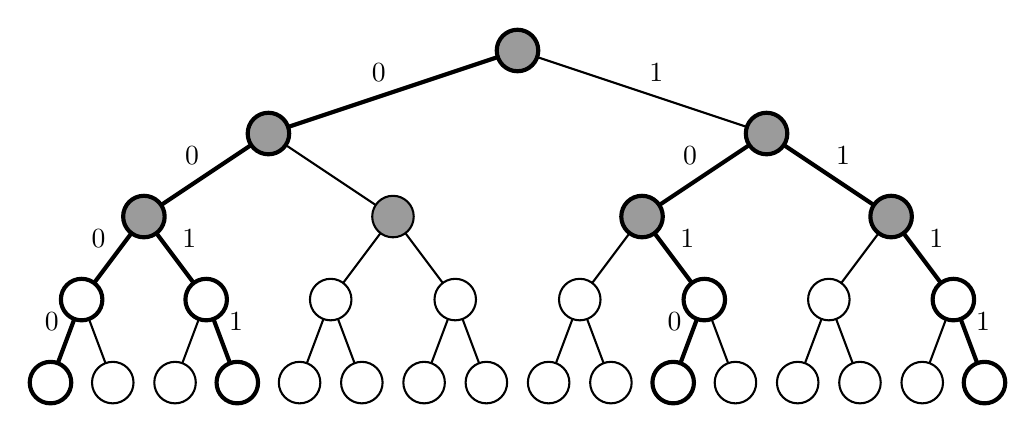
\begin{tikzpicture}[x=0.75pt,y=0.75pt,yscale=-1,xscale=1]
%uncomment if require: \path (0,196); %set diagram left start at 0, and has height of 196

%Straight Lines [id:da18030786969741874] 
\draw [line width=1.5]    (235,10) -- (115,50) ;
%Straight Lines [id:da08184252066372677] 
\draw    (235,10) -- (355,50) ;
%Straight Lines [id:da6695423787123118] 
\draw [line width=1.5]    (25,130) -- (10,170) ;
%Straight Lines [id:da8776558920239244] 
\draw    (25,130) -- (40,170) ;
%Straight Lines [id:da456480770871897] 
\draw    (85,130) -- (70,170) ;
%Straight Lines [id:da24213870313796404] 
\draw [line width=1.5]    (85,130) -- (100,170) ;
%Straight Lines [id:da6422874840426858] 
\draw    (145,130) -- (130,170) ;
%Straight Lines [id:da03506691074715662] 
\draw [line width=0.75]    (145,130) -- (160,170) ;
%Straight Lines [id:da06640681512096891] 
\draw    (205,130) -- (190,170) ;
%Straight Lines [id:da5432180850374912] 
\draw    (205,130) -- (220,170) ;
%Straight Lines [id:da9508663907107122] 
\draw [line width=1.5]    (55,90) -- (25,130) ;
%Straight Lines [id:da9754036077349393] 
\draw [line width=1.5]    (55,90) -- (85,130) ;
%Straight Lines [id:da17473830580335048] 
\draw [line width=0.75]    (175,90) -- (145,130) ;
%Straight Lines [id:da24977957224163605] 
\draw    (175,90) -- (205,130) ;
%Straight Lines [id:da7576985148237267] 
\draw [line width=1.5]    (115,50) -- (55,90) ;
%Straight Lines [id:da42857534612705006] 
\draw [line width=0.75]    (115,50) -- (175,90) ;
%Shape: Circle [id:dp03905566301592911] 
\draw  [fill={rgb, 255:red, 255; green, 255; blue, 255 }  ,fill opacity=1 ][line width=1.5]  (0,170) .. controls (0,164.48) and (4.48,160) .. (10,160) .. controls (15.52,160) and (20,164.48) .. (20,170) .. controls (20,175.52) and (15.52,180) .. (10,180) .. controls (4.48,180) and (0,175.52) .. (0,170) -- cycle ;
%Shape: Circle [id:dp09712081988307864] 
\draw  [fill={rgb, 255:red, 255; green, 255; blue, 255 }  ,fill opacity=1 ][line width=0.75]  (30,170) .. controls (30,164.48) and (34.48,160) .. (40,160) .. controls (45.52,160) and (50,164.48) .. (50,170) .. controls (50,175.52) and (45.52,180) .. (40,180) .. controls (34.48,180) and (30,175.52) .. (30,170) -- cycle ;
%Shape: Circle [id:dp08628380634376609] 
\draw  [fill={rgb, 255:red, 255; green, 255; blue, 255 }  ,fill opacity=1 ][line width=0.75]  (60,170) .. controls (60,164.48) and (64.48,160) .. (70,160) .. controls (75.52,160) and (80,164.48) .. (80,170) .. controls (80,175.52) and (75.52,180) .. (70,180) .. controls (64.48,180) and (60,175.52) .. (60,170) -- cycle ;
%Shape: Circle [id:dp8302838626680549] 
\draw  [fill={rgb, 255:red, 255; green, 255; blue, 255 }  ,fill opacity=1 ][line width=1.5]  (90,170) .. controls (90,164.48) and (94.48,160) .. (100,160) .. controls (105.52,160) and (110,164.48) .. (110,170) .. controls (110,175.52) and (105.52,180) .. (100,180) .. controls (94.48,180) and (90,175.52) .. (90,170) -- cycle ;
%Shape: Circle [id:dp8706292046593302] 
\draw  [fill={rgb, 255:red, 255; green, 255; blue, 255 }  ,fill opacity=1 ][line width=0.75]  (120,170) .. controls (120,164.48) and (124.48,160) .. (130,160) .. controls (135.52,160) and (140,164.48) .. (140,170) .. controls (140,175.52) and (135.52,180) .. (130,180) .. controls (124.48,180) and (120,175.52) .. (120,170) -- cycle ;
%Shape: Circle [id:dp4559690350844394] 
\draw  [fill={rgb, 255:red, 255; green, 255; blue, 255 }  ,fill opacity=1 ][line width=0.75]  (150,170) .. controls (150,164.48) and (154.48,160) .. (160,160) .. controls (165.52,160) and (170,164.48) .. (170,170) .. controls (170,175.52) and (165.52,180) .. (160,180) .. controls (154.48,180) and (150,175.52) .. (150,170) -- cycle ;
%Shape: Circle [id:dp5597760850046549] 
\draw  [fill={rgb, 255:red, 255; green, 255; blue, 255 }  ,fill opacity=1 ][line width=0.75]  (180,170) .. controls (180,164.48) and (184.48,160) .. (190,160) .. controls (195.52,160) and (200,164.48) .. (200,170) .. controls (200,175.52) and (195.52,180) .. (190,180) .. controls (184.48,180) and (180,175.52) .. (180,170) -- cycle ;
%Shape: Circle [id:dp5747757446149799] 
\draw  [fill={rgb, 255:red, 255; green, 255; blue, 255 }  ,fill opacity=1 ][line width=0.75]  (210,170) .. controls (210,164.48) and (214.48,160) .. (220,160) .. controls (225.52,160) and (230,164.48) .. (230,170) .. controls (230,175.52) and (225.52,180) .. (220,180) .. controls (214.48,180) and (210,175.52) .. (210,170) -- cycle ;
%Shape: Circle [id:dp13687363238538053] 
\draw  [fill={rgb, 255:red, 255; green, 255; blue, 255 }  ,fill opacity=1 ][line width=1.5]  (15,130) .. controls (15,124.48) and (19.48,120) .. (25,120) .. controls (30.52,120) and (35,124.48) .. (35,130) .. controls (35,135.52) and (30.52,140) .. (25,140) .. controls (19.48,140) and (15,135.52) .. (15,130) -- cycle ;
%Shape: Circle [id:dp19347578364499673] 
\draw  [fill={rgb, 255:red, 255; green, 255; blue, 255 }  ,fill opacity=1 ][line width=1.5]  (75,130) .. controls (75,124.48) and (79.48,120) .. (85,120) .. controls (90.52,120) and (95,124.48) .. (95,130) .. controls (95,135.52) and (90.52,140) .. (85,140) .. controls (79.48,140) and (75,135.52) .. (75,130) -- cycle ;
%Shape: Circle [id:dp3599355587088173] 
\draw  [fill={rgb, 255:red, 255; green, 255; blue, 255 }  ,fill opacity=1 ][line width=0.75]  (135,130) .. controls (135,124.48) and (139.48,120) .. (145,120) .. controls (150.52,120) and (155,124.48) .. (155,130) .. controls (155,135.52) and (150.52,140) .. (145,140) .. controls (139.48,140) and (135,135.52) .. (135,130) -- cycle ;
%Shape: Circle [id:dp5908856368176647] 
\draw  [fill={rgb, 255:red, 255; green, 255; blue, 255 }  ,fill opacity=1 ][line width=0.75]  (195,130) .. controls (195,124.48) and (199.48,120) .. (205,120) .. controls (210.52,120) and (215,124.48) .. (215,130) .. controls (215,135.52) and (210.52,140) .. (205,140) .. controls (199.48,140) and (195,135.52) .. (195,130) -- cycle ;
%Shape: Circle [id:dp41209359565693915] 
\draw  [fill={rgb, 255:red, 155; green, 155; blue, 155 }  ,fill opacity=1 ][line width=1.5]  (45,90) .. controls (45,84.48) and (49.48,80) .. (55,80) .. controls (60.52,80) and (65,84.48) .. (65,90) .. controls (65,95.52) and (60.52,100) .. (55,100) .. controls (49.48,100) and (45,95.52) .. (45,90) -- cycle ;
%Shape: Circle [id:dp009399054741537904] 
\draw  [fill={rgb, 255:red, 155; green, 155; blue, 155 }  ,fill opacity=1 ][line width=0.75]  (165,90) .. controls (165,84.48) and (169.48,80) .. (175,80) .. controls (180.52,80) and (185,84.48) .. (185,90) .. controls (185,95.52) and (180.52,100) .. (175,100) .. controls (169.48,100) and (165,95.52) .. (165,90) -- cycle ;
%Shape: Circle [id:dp528073778475892] 
\draw  [fill={rgb, 255:red, 155; green, 155; blue, 155 }  ,fill opacity=1 ][line width=1.5]  (105,50) .. controls (105,44.48) and (109.48,40) .. (115,40) .. controls (120.52,40) and (125,44.48) .. (125,50) .. controls (125,55.52) and (120.52,60) .. (115,60) .. controls (109.48,60) and (105,55.52) .. (105,50) -- cycle ;
%Straight Lines [id:da11852362945611472] 
\draw    (265,130) -- (250,170) ;
%Straight Lines [id:da5591497670415919] 
\draw    (265,130) -- (280,170) ;
%Straight Lines [id:da1401309606957788] 
\draw [line width=1.5]    (325,130) -- (310,170) ;
%Straight Lines [id:da6644822016715766] 
\draw    (325,130) -- (340,170) ;
%Straight Lines [id:da615803123899757] 
\draw    (385,130) -- (370,170) ;
%Straight Lines [id:da4594242880739903] 
\draw [line width=0.75]    (385,130) -- (400,170) ;
%Straight Lines [id:da7326524647487114] 
\draw    (445,130) -- (430,170) ;
%Straight Lines [id:da11271665375045803] 
\draw [line width=1.5]    (445,130) -- (460,170) ;
%Straight Lines [id:da6713398753370163] 
\draw    (295,90) -- (265,130) ;
%Straight Lines [id:da9911783089548187] 
\draw [line width=1.5]    (295,90) -- (325,130) ;
%Straight Lines [id:da20755832049249] 
\draw [line width=0.75]    (415,90) -- (385,130) ;
%Straight Lines [id:da6670171480483362] 
\draw [line width=1.5]    (415,90) -- (445,130) ;
%Straight Lines [id:da6886428816533332] 
\draw [line width=1.5]    (355,50) -- (295,90) ;
%Straight Lines [id:da39314609681321877] 
\draw [line width=1.5]    (355,50) -- (415,90) ;
%Shape: Circle [id:dp7753000345940457] 
\draw  [fill={rgb, 255:red, 255; green, 255; blue, 255 }  ,fill opacity=1 ][line width=0.75]  (240,170) .. controls (240,164.48) and (244.48,160) .. (250,160) .. controls (255.52,160) and (260,164.48) .. (260,170) .. controls (260,175.52) and (255.52,180) .. (250,180) .. controls (244.48,180) and (240,175.52) .. (240,170) -- cycle ;
%Shape: Circle [id:dp4802713208709277] 
\draw  [fill={rgb, 255:red, 255; green, 255; blue, 255 }  ,fill opacity=1 ][line width=0.75]  (270,170) .. controls (270,164.48) and (274.48,160) .. (280,160) .. controls (285.52,160) and (290,164.48) .. (290,170) .. controls (290,175.52) and (285.52,180) .. (280,180) .. controls (274.48,180) and (270,175.52) .. (270,170) -- cycle ;
%Shape: Circle [id:dp13339622257445383] 
\draw  [fill={rgb, 255:red, 255; green, 255; blue, 255 }  ,fill opacity=1 ][line width=1.5]  (300,170) .. controls (300,164.48) and (304.48,160) .. (310,160) .. controls (315.52,160) and (320,164.48) .. (320,170) .. controls (320,175.52) and (315.52,180) .. (310,180) .. controls (304.48,180) and (300,175.52) .. (300,170) -- cycle ;
%Shape: Circle [id:dp725595936684422] 
\draw  [fill={rgb, 255:red, 255; green, 255; blue, 255 }  ,fill opacity=1 ][line width=0.75]  (330,170) .. controls (330,164.48) and (334.48,160) .. (340,160) .. controls (345.52,160) and (350,164.48) .. (350,170) .. controls (350,175.52) and (345.52,180) .. (340,180) .. controls (334.48,180) and (330,175.52) .. (330,170) -- cycle ;
%Shape: Circle [id:dp8260566334335642] 
\draw  [fill={rgb, 255:red, 255; green, 255; blue, 255 }  ,fill opacity=1 ][line width=0.75]  (360,170) .. controls (360,164.48) and (364.48,160) .. (370,160) .. controls (375.52,160) and (380,164.48) .. (380,170) .. controls (380,175.52) and (375.52,180) .. (370,180) .. controls (364.48,180) and (360,175.52) .. (360,170) -- cycle ;
%Shape: Circle [id:dp39960075028076947] 
\draw  [fill={rgb, 255:red, 255; green, 255; blue, 255 }  ,fill opacity=1 ][line width=0.75]  (390,170) .. controls (390,164.48) and (394.48,160) .. (400,160) .. controls (405.52,160) and (410,164.48) .. (410,170) .. controls (410,175.52) and (405.52,180) .. (400,180) .. controls (394.48,180) and (390,175.52) .. (390,170) -- cycle ;
%Shape: Circle [id:dp8132641785887298] 
\draw  [fill={rgb, 255:red, 255; green, 255; blue, 255 }  ,fill opacity=1 ][line width=0.75]  (420,170) .. controls (420,164.48) and (424.48,160) .. (430,160) .. controls (435.52,160) and (440,164.48) .. (440,170) .. controls (440,175.52) and (435.52,180) .. (430,180) .. controls (424.48,180) and (420,175.52) .. (420,170) -- cycle ;
%Shape: Circle [id:dp48883984021614624] 
\draw  [fill={rgb, 255:red, 255; green, 255; blue, 255 }  ,fill opacity=1 ][line width=1.5]  (450,170) .. controls (450,164.48) and (454.48,160) .. (460,160) .. controls (465.52,160) and (470,164.48) .. (470,170) .. controls (470,175.52) and (465.52,180) .. (460,180) .. controls (454.48,180) and (450,175.52) .. (450,170) -- cycle ;
%Shape: Circle [id:dp6411714596707287] 
\draw  [fill={rgb, 255:red, 255; green, 255; blue, 255 }  ,fill opacity=1 ][line width=0.75]  (255,130) .. controls (255,124.48) and (259.48,120) .. (265,120) .. controls (270.52,120) and (275,124.48) .. (275,130) .. controls (275,135.52) and (270.52,140) .. (265,140) .. controls (259.48,140) and (255,135.52) .. (255,130) -- cycle ;
%Shape: Circle [id:dp30417580383311815] 
\draw  [fill={rgb, 255:red, 255; green, 255; blue, 255 }  ,fill opacity=1 ][line width=1.5]  (315,130) .. controls (315,124.48) and (319.48,120) .. (325,120) .. controls (330.52,120) and (335,124.48) .. (335,130) .. controls (335,135.52) and (330.52,140) .. (325,140) .. controls (319.48,140) and (315,135.52) .. (315,130) -- cycle ;
%Shape: Circle [id:dp3363829552561317] 
\draw  [fill={rgb, 255:red, 255; green, 255; blue, 255 }  ,fill opacity=1 ][line width=0.75]  (375,130) .. controls (375,124.48) and (379.48,120) .. (385,120) .. controls (390.52,120) and (395,124.48) .. (395,130) .. controls (395,135.52) and (390.52,140) .. (385,140) .. controls (379.48,140) and (375,135.52) .. (375,130) -- cycle ;
%Shape: Circle [id:dp7502474616403281] 
\draw  [fill={rgb, 255:red, 255; green, 255; blue, 255 }  ,fill opacity=1 ][line width=1.5]  (435,130) .. controls (435,124.48) and (439.48,120) .. (445,120) .. controls (450.52,120) and (455,124.48) .. (455,130) .. controls (455,135.52) and (450.52,140) .. (445,140) .. controls (439.48,140) and (435,135.52) .. (435,130) -- cycle ;
%Shape: Circle [id:dp5803858053866973] 
\draw  [fill={rgb, 255:red, 155; green, 155; blue, 155 }  ,fill opacity=1 ][line width=1.5]  (285,90) .. controls (285,84.48) and (289.48,80) .. (295,80) .. controls (300.52,80) and (305,84.48) .. (305,90) .. controls (305,95.52) and (300.52,100) .. (295,100) .. controls (289.48,100) and (285,95.52) .. (285,90) -- cycle ;
%Shape: Circle [id:dp3607270758887733] 
\draw  [fill={rgb, 255:red, 155; green, 155; blue, 155 }  ,fill opacity=1 ][line width=1.5]  (405,90) .. controls (405,84.48) and (409.48,80) .. (415,80) .. controls (420.52,80) and (425,84.48) .. (425,90) .. controls (425,95.52) and (420.52,100) .. (415,100) .. controls (409.48,100) and (405,95.52) .. (405,90) -- cycle ;
%Shape: Circle [id:dp6027653601523095] 
\draw  [fill={rgb, 255:red, 155; green, 155; blue, 155 }  ,fill opacity=1 ][line width=1.5]  (345,50) .. controls (345,44.48) and (349.48,40) .. (355,40) .. controls (360.52,40) and (365,44.48) .. (365,50) .. controls (365,55.52) and (360.52,60) .. (355,60) .. controls (349.48,60) and (345,55.52) .. (345,50) -- cycle ;
%Shape: Circle [id:dp7293505921502836] 
\draw  [fill={rgb, 255:red, 155; green, 155; blue, 155 }  ,fill opacity=1 ][line width=1.5]  (225,10) .. controls (225,4.48) and (229.48,0) .. (235,0) .. controls (240.52,0) and (245,4.48) .. (245,10) .. controls (245,15.52) and (240.52,20) .. (235,20) .. controls (229.48,20) and (225,15.52) .. (225,10) -- cycle ;

% Text Node
\draw (173,26.6) node [anchor=south east] [inner sep=0.75pt]    {$0$};
% Text Node
\draw (297,26.6) node [anchor=south west] [inner sep=0.75pt]    {$1$};
% Text Node
\draw (83,66.6) node [anchor=south east] [inner sep=0.75pt]    {$0$};
% Text Node
\draw (38,106.6) node [anchor=south east] [inner sep=0.75pt]    {$0$};
% Text Node
\draw (15.5,146.6) node [anchor=south east] [inner sep=0.75pt]    {$0$};
% Text Node
\draw (323,66.6) node [anchor=south east] [inner sep=0.75pt]    {$0$};
% Text Node
\draw (315.5,146.6) node [anchor=south east] [inner sep=0.75pt]    {$0$};
% Text Node
\draw (72,106.6) node [anchor=south west] [inner sep=0.75pt]    {$1$};
% Text Node
\draw (94.5,146.6) node [anchor=south west] [inner sep=0.75pt]    {$1$};
% Text Node
\draw (312,106.6) node [anchor=south west] [inner sep=0.75pt]    {$1$};
% Text Node
\draw (387,66.6) node [anchor=south west] [inner sep=0.75pt]    {$1$};
% Text Node
\draw (432,106.6) node [anchor=south west] [inner sep=0.75pt]    {$1$};
% Text Node
\draw (454.5,146.6) node [anchor=south west] [inner sep=0.75pt]    {$1$};


\end{tikzpicture}
  \caption{混合$2$中$\ell=4$时的评估树。被阴影着色的结点被分配了随机标签,未被着色的结点被分配了派生标签。加粗的路径对应于输入 $0000$,$0011$,$1010$ 和 $1111$。}
  \label{fig:4-16}
\end{figure}

显然,混合 $0$ 等同于攻击游戏 \ref{game:4-2} 的实验 $0$,而混合 $\ell$ 等同于实验 $1$。直观地说,在假设 $G$ 是一个安全的 PRG 的情况下,对于 $j=0,\dots,\ell-1$,对手应该无法分辨混合 $j$ 和混合 $j+1$。在严格表述这一想法的时候,我们必须要注意,评估树可能是非常巨大的,为了建立一个有效的攻击 $G$ 的 PRG 对手,我们无法负担写下整棵树的开销(甚至是写下树中的一层的开销)。相对地,我们需要利用这样一个事实,即如果 PRF 对手最多向其挑战者发起 $Q$ 次查询(这是一个多项式边界的值),那么在评估树的任何一层 $j$,这 $Q$ 次查询所跟踪的路径最多会涉及 $Q$ 个 $j$ 层中的结点(在图 \ref{fig:4-16} 中,对于给定的输入,应当是第$2$层的第一、第三和第四个结点)。我们构建的 PRG 对手会根据需要使用``忠实的侏儒"思路的一个变体来有效地维护第 $j$ 层的相关随机标签。
\end{proof}

\begin{proof}
令 $\mathcal{A}$ 是一个有效对手,它就 $F$ 进行攻击游戏 \ref{game:4-2} 中的攻击。我们假设 $\mathcal{A}$ 最多向其挑战者发起 $Q$ 次查询,其中 $Q$ 是一个多项式边界的值。

如上所述,我们定义 $\ell+1$ 个混合游戏:混合$0$,$\dots$,混合$\ell$,其中每个游戏都在 $\mathcal{A}$ 和一个挑战者之间进行。在混合 $j$ 中,挑战者的工作方式如下:

\vspace{5pt}

\hspace*{5pt} 选取 $f\overset{\rm R}\leftarrow{\rm Funs}[\{0,1\}^j,\mathcal{S}]$\\
\hspace*{26pt} 当从 $\mathcal{A}$ 处收到查询 $x=(a_1,\dots,a_\ell)\in\{0,1\}^\ell$ 时:\\
\hspace*{50pt} 令 $u\leftarrow(a_1,\dots,a_j)$,$v\leftarrow(a_{j+1},\dots,a_\ell)$\\
\hspace*{50pt} 令 $y\leftarrow G^*(f(u),v)$\\
\hspace*{50pt} 将 $y$ 发送给 $\mathcal{A}$。

\vspace{5pt}

\noindent
直观地说,对于 $u\in\{0,1\}^j$,$f(u)$ 代表 $u$ 所寻址的第 $j$ 层结点的随机标签。因此,第 $j$ 层的每个结点都会被分配一个随机标签,而第 $j+1$ 层到第 $l$ 层的结点都会被分配派生标签。请注意,在我们对混合游戏的描述中,我们没有明确地给第 $0$ 层到第 $j-1$ 层的结点分配标签,因为这些标签不影响任何输出。

对于 $j=0,\dots,\ell$,由于混合 $0$ 相当于攻击游戏 \ref{game:4-2} 的实验 $0$,而混合 $\ell$ 相当于实验 $1$,我们有:
\begin{equation}\label{eq:4-30}
{\rm PRF\mathsf{adv}}[\mathcal{A},F]=|p_\ell-p_0|
\end{equation}

用 $G'$ 表示 $G$ 的 $Q$ 次并行组合,如我们在 \ref{subsec:3-4-1} 小节中介绍过的那样。$G'$ 以 $(s_1,\dots,s_Q)\in\mathcal{S}^Q$ 为输入,输出 $(G(s_1),\dots,G(s_Q))\in(\mathcal{S}^2)^Q$。根据定理 \ref{theo:3-2},如果 $G$ 是一个安全的 PRG,那么 $G'$ 也是一个安全的 PRG。

现在,我们建立一个有效 PRG 对手 $\mathcal{B}'$ 来攻击 $G'$,使得:
\begin{equation}\label{eq:4-31}
{\rm PRG\mathsf{adv}}[\mathcal{B}',G']=\frac{1}{\ell}\cdot|p_\ell-p_0|
\end{equation}
我们首先概述 $\mathcal{B}'$ 的工作原理。在针对 $G'$ 进行攻击游戏 \ref{game:3-1} 中的攻击时,挑战者向 $\mathcal{B}'$ 提出一个向量:
\begin{equation}\label{eq:4-32}
\vec{r}=((r_{10},r_{11}),\dots,(r_{Q0},r_{Q1}))\in(\mathcal{S}^2)^Q
\end{equation}
在攻击游戏的实验 $0$ 中,对于随机的 $\vec{s}\in\mathcal{S}^Q$,有 $\vec{r}=G(\vec{s})$。而在实验 $1$ 中,$\vec{r}$ 是从 $(\mathcal{S}^2)^Q$ 中随机选出的。为了区分这两个实验,$\mathcal{B}'$ 随机选择一个 $\omega\in\{1,\dots,\ell\}$,并扮演 $\mathcal{A}$ 的挑战者的角色,并使用 $\vec r$ 的元素按顺序给评估树的第 $\omega$ 层的结点打上标签。为此,$\mathcal{B}'$ 需要维护一张查找表,这使得它可以将每某个查询 $x\in\{0,1\}^\ell$ 的每个前缀 $u\in\{0,1\}^{\omega-1}$ 与一个索引 $p$ 关联起来,这样,由 $u$ 寻址的结点的子结点就被种子对 $(r_{p0},r_{p1})$ 标记。最后,当 $\mathcal{A}$ 终止并输出一个比特时,$\mathcal{B}'$ 就输出相同的比特。从 $\mathcal{B}'$ 的构造细节可以看出,对于任何固定的 $j=1,\dots,\ell$,以 $\omega=j$ 为条件,$\mathcal{B}'$ 输出 $1$ 的概率为:
\begin{itemize}
	\item $p_{j-1}$,如果 $\mathcal{B}'$ 处于其攻击游戏的实验 $0$ 中,或
	\item $p_j$,如果 $\mathcal{B}'$ 处于其攻击游戏的实验 $1$ 中。
\end{itemize}
然后通过简单的放缩计算,我们就能得到式 \ref{eq:4-31}。

下面我们来说说细节。我们将查找表实现为一个关联数组 $Map:\{0,1\}^*\to\mathbb{Z}_{>0}$。下面是 $\mathcal{B}'$ 的工作原理:

\vspace{5pt}

\hspace*{5pt} 当从挑战者处收到如式 \ref{eq:4-32} 的向量 $\vec r$ 时,$\mathcal{B}'$ 扮演 $\mathcal{A}$ 的挑战者的角色,如下所示:\\
\hspace*{50pt} 选取 $\omega\overset{\rm R}\leftarrow\{1,\dots,\ell\}$\\
\hspace*{50pt} 初始化一个空关联数组 $Map:\{0,1\}^*\to\mathbb{Z}_{>0}$\\
\hspace*{50pt} 令 $ctr\leftarrow 0$\\
\hspace*{50pt} 当从 $\mathcal{A}$ 处收到一个查询 $x=(a_1,\dots,a_\ell)\in\{0,1\}^\ell$ 时:\\
\hspace*{75pt} 令 $u\leftarrow(a_1,\dots,a_{\omega-1})$,$d\leftarrow a_\omega$,$v\leftarrow(a_{\omega+1},\dots,a_\ell)$\\
\hspace*{75pt} 如果 $u\notin{\rm Domain}(Map)$:\\
\hspace*{100pt} 令 $ctr\leftarrow ctr+1$,$Map[u]\leftarrow ctr$\\
\hspace*{75pt} 令 $p\leftarrow Map[u]$,$y\leftarrow G^*(r_{pd},v)$\\
\hspace*{75pt} 将 $y$ 发送给 $\mathcal{A}$。

\vspace{3pt}

\hspace*{5pt} 最后,$\mathcal{B}'$ 输出 $\mathcal{A}$ 所输出的任何东西。

\vspace{5pt}

对于$b=0,1$,令 $W_b$ 为 $\mathcal{B}'$ 就 $G'$ 在攻击游戏 \ref{game:3-1} 的实验 $b$ 中输出 $1$ 的事件。我们声称,对于任何固定的 $j=1,\dots,\ell$,都有:
\[
\Pr[W_0|\omega=j]=p_{j-1},
\quad
\Pr[W_1|\omega=j]=p_j
\]
事实上,以 $\omega=j$ 为条件,对于固定的 $j$,考虑 $\mathcal{B}'$ 如何给评估树中的结点加标签。一方面,当 $\mathcal{B}'$ 处于其攻击游戏的实验 $1$ 时,它可以有效地给第 $j$ 层的结点分配随机标签,而查找表能够确保这些标签不会重复。另一方面,当 $\mathcal{B}'$ 处于其攻击游戏的实验 $0$ 时,它可以有效地给第 $j$ 层的结点分配伪随机标签,这等于给这些结点在第 $j-1$ 层的父结点分配随机标签,并在第 $j$ 层分配派生标签;同样,查找表能够确保标签不会重复。

基于上述声称,我们可以通过一个简单的放缩计算得到式 \ref{eq:4-31}:
\[
\begin{aligned}
{\rm PRG\mathsf{adv}}[\mathcal{B}',G']
&=|\Pr[W_1]-\Pr[W_0]|\\
&=\frac{1}{\ell}\cdot\Big\lvert\sum_{j=1}^\ell\Pr[W_1\,|\,\omega=j]-\sum_{j=1}^\ell\Pr[W_0\,|\,\omega=j]\Big\rvert\\
&=\frac{1}{\ell}\cdot\Big\lvert\sum_{j=1}^\ell p_j-\sum_{j=1}^\ell p_{j-1}\Big\rvert\\
&=\frac{1}{\ell}\cdot|p_\ell-p_0|
\end{aligned}
\]

最后,根据定理 \ref{theo:3-2},必然存在一个有效 PRG 对手 $\mathcal{B}$,使得:
\begin{equation}\label{eq:4-33}
{\rm PRG\mathsf{adv}}[\mathcal{B}',G']=Q\cdot{\rm PRG\mathsf{adv}}[\mathcal{B},G]
\end{equation}
现在,结合式 \ref{eq:4-30},\ref{eq:4-31} 和 \ref{eq:4-33},可以得到该定理。
\end{proof}

\subsection{变长树构造}

很自然地,我们下面考虑树构造如何在可变长度的输入上工作。和之前一样,令 $G$ 是一个定义在 $(\mathcal{S},\mathcal{S}^2)$ 上的 PRG,$G^*$ 的定义与之前也一样。对于任何多项式边界值 $\ell$,我们定义 PRF $\tilde F$,其密钥空间为 $\mathcal{S}$,输入空间为 $\{0,1\}^{\leq l}$,输出空间为 $\mathcal{S}$,对于 $s\in\mathcal{S}$ 和 $x\in\{0,1\}^{\leq\ell}$,我们定义:
\[
\tilde F(s,x)=G^*(s,x)
\]

不幸的是,$\tilde F$ 不是一个安全的 PRF,原因是存在着一种平凡的\textbf{扩展攻击 (extension attack)}。假设 $u,v\in\{0,1\}^{\leq\ell}$,其中 $u$ 是 $v$ 的真前缀,即存在非空序列 $w$ 使得 $v=u\,\Vert\,w$。那么,给定 $u$,$v$ 以及 $y:=\tilde F(s,u)$,我们很容易基于 $G^*(y,w)$ 计算 $F(s,v)$。当然,对于一个真随机函数来说,给定 $u$ 处的值,我们无法预测它在 $v$ 处的值。因此,我们很容易将 $\tilde F(s,\cdot)$ 与一个真随机函数区分开来。

即便 $\tilde F$ 不是一个安全的 PRF,我们仍然可以得出一些关于它的有趣结论。我们下面表明,针对特定的受限对手所组成的集合,$\tilde F$ 是一个 PRF,这种对手被称为\textbf{无前缀对手 (prefix-free adversaries)}。

\begin{definition}\label{def:4-5}
令 $F$ 是一个定义在 $(\mathcal{K},\mathcal{X}^{\leq\ell}, \mathcal{Y})$ 上的 PRF。对于一个就 $F$ 进行攻击游戏 \ref{game:4-2} 中的攻击的 PRF 对手 $\mathcal{A}$,如果它所发出的所有查询都是 $\mathcal{X}$ 上长度不超过 $\ell$ 的非空序列,且其中任何一个查询都不是其他查询的真前缀\footnote[3]{对于序列 $x=(a_1\dots a_s)$ 和 $y=(b_1\dots b_t)$,如果 $s\leq t$,且对于 $i=1,\dots,s$ 都有 $a_i=b_i$,我们就称 $x$ 是 $y$ 的一个\textbf{前缀};在此基础上,如果 $s<t$,我们就称 $x$ 是 $y$ 的一个\textbf{真前缀(proper prefix)}。},我们就称这样的对手 $\mathcal{A}$ 是一个\textbf{无前缀对手 (prefix-free adversary)}。我们将 $\mathcal{A}$ 赢得游戏的优势记为 ${\rm PRF^{pf}\mathsf{adv}}[\mathcal{A},F]$。此外,如果对于所有有效的无前缀对手 $\mathcal{A}$,${\rm PRF^{pf}\mathsf{adv}}[\mathcal{A},F]$ 的值都可忽略不计,我们就称 $F$ 是一个\textbf{无前缀安全的 PRF (prefix-free secure PRF)}。
\end{definition}

比如,如果一个无前缀对手对序列 $(a_1,a_2,a_3)$ 发起查询,那么它就不能再对 $(a_1)$ 和 $(a_1,a_2)$ 发起查询。

\begin{theorem}\label{theo:4-11}
如果 $G$ 是一个安全 PRG,那么由 $G$ 派生的变长树构造 $\tilde F$ 是一个无前缀安全的 PRF。
\begin{quote}
特别地,对于每个就 $\tilde F$ 进行攻击游戏 \ref{game:4-2} 的无前缀对手 $\mathcal{A}$,如果它最多能向其挑战者发起 $Q$ 次查询,那么必然存在一个就 $G$ 进行攻击游戏 \ref{game:3-1} 的 PRG 对手 $\mathcal{B}$,其中 $\mathcal{B}$ 是一个围绕 $\mathcal{A}$ 的基本包装器,满足:
\end{quote}
\[
{\rm PRF^{pf}\mathsf{adv}}[\mathcal{A},\tilde{F}]=\ell Q\cdot{\rm PRG\mathsf{adv}}[\mathcal{B},G]
\]
\end{theorem}

\begin{proof}
该证明的基本思路与定理 \ref{theo:4-10} 完全相同。我们在此仅简述主要观点,并强调与那个证明的不同之处。

令 $\mathcal{A}$ 是一个有效的无前缀对手,它就 $\tilde F$ 进行攻击游戏 \ref{game:4-2}。假设 $\mathcal{A}$ 最多向其挑战者发起 $Q$ 次查询。此外,为了方便起见,我们假设 $\mathcal{A}$ 发起的任意两次查询都不相同,也不会出现其中一个是另一个的前缀的情况。攻击游戏 \ref{game:4-2} 中的挑战者不需要强制服从这一假设,我们只是假设 $\mathcal{A}$ 在按规则行事。

和之前一样,我们用一棵评估树来考察 $\tilde F(s,\cdot)$ 的计算:其根结点的标签为 $s$,所有其他结点的标签都是派生标签。现在唯一的区别是,$\tilde F(s,\cdot)$ 的输入也可以寻址到评估树的\emph{内部}结点。然而,无前缀的约束意味着,没有任何一个输入可以寻址到一个由之前输入所寻址的结点的祖先结点。

我们再次定义 $\ell$ 个混合游戏:混合$0$,$\dots$,混合$\ell$。在这些游戏中,挑战者使用的评估树的标记方式与定理 \ref{theo:4-10} 的证明中完全相同:在混合 $j$ 中,第 $0$ 层到第 $j$ 层的结点被分配随机标签,而其他层的结点被分配派生标签。挑战者对查询 $x$ 的应答是返回评估树中 $x$ 所寻址的结点的标签,注意该结点现在不一定是叶子结点。更正式地说,混合 $j$ 中的挑战者的工作方式如下:

\vspace{5pt}

\hspace*{5pt} 选取 $f\overset{\rm R}\leftarrow{\rm Funs}[\{0,1\}^{\leq j},\mathcal{S}]$\\
\hspace*{26pt} 当从 $\mathcal{A}$ 处收到查询 $x=(a_1,\dots,a_n)\in\{0,1\}^\ell$ 时:\\
\hspace*{50pt} 如果 $n<j$:\\
\hspace*{75pt} 则令 $y\leftarrow f(x)$\\
\hspace*{75pt} 否则令 $u\leftarrow(a_1,\dots,a_j)$,$v\leftarrow(a_{j+1},\dots,a_n)$,$y\leftarrow G^*(f(u),v)$\\
\hspace*{50pt} 将 $y$ 发送给 $\mathcal{A}$。

\vspace{5pt}

\noindent
对于$j=0,\dots,l$,定义 $p_j$ 为 $\mathcal{A}$ 在混合 $j$ 中输出 $1$ 的概率。读者很容易验证,我们有:
\[
{\rm PRF^{pf}\mathsf{adv}}[\mathcal{A},\tilde{F}]=|p_\ell-p_0|
\]

接下来,我们定义一个攻击 $G$ 的 $Q$ 次并行组合 $G'$ 的有效 PRG 对手 $\mathcal{B}'$,使得:
\[
{\rm PRG}\mathsf{adv}[\mathcal{B}',G']=\frac{1}{\ell}\cdot|p_\ell-p_0|
\]
对手 $\mathcal{B}'$ 的工作方式如下:

\vspace{5pt}

\hspace*{5pt} 当从挑战者处收到如式 \ref{eq:4-32} 的向量 $\vec r$ 时,$\mathcal{B}'$ 扮演 $\mathcal{A}$ 的挑战者的角色,如下所示:\\
\hspace*{50pt} 选取 $\omega\overset{\rm R}\leftarrow\{1,\dots,\ell\}$\\
\hspace*{50pt} 初始化一个空关联数组 $Map:\{0,1\}^*\to\mathbb{Z}_{>0}$\\
\hspace*{50pt} 令 $ctr\leftarrow 0$\\
\hspace*{50pt} 当从 $\mathcal{A}$ 处收到一个查询 $x=(a_1,\dots,a_n)\in\{0,1\}^\ell$ 时:\\
\hspace*{75pt} 如果 $n<\omega$:\\
\hspace*{11pt} ($*$)
\hspace*{69pt} 选取 $y\overset{\rm R}\leftarrow\mathcal{S}$\\
\hspace*{75pt} 否则:\\
\hspace*{100pt} 令 $u\leftarrow(a_1,\dots,a_{\omega-1})$,$d\leftarrow a_\omega$,$v\leftarrow(a_{\omega+1},\dots,a_n)$\\
\hspace*{100pt} 如果 $u\notin{\rm Domain}(Map)$:\\
\hspace*{125pt} 令 $ctr\leftarrow ctr+1$,$Map[u]\leftarrow ctr$\\
\hspace*{100pt} 令 $p\leftarrow Map[u]$,$y\leftarrow G^*(r_{pd},v)$\\
\hspace*{75pt} 将 $y$ 发送给 $\mathcal{A}$。

\vspace{3pt}

\hspace*{5pt} 最后,$\mathcal{B}'$ 输出 $\mathcal{A}$ 所输出的任何东西。

\vspace{5pt}

对于 $b=0,1$,记 $W_b$ 为 $\mathcal{B}'$ 就 $G'$ 在攻击游戏 \ref{game:4-2} 的实验 $b$ 中输出 $1$ 的事件。不难看出,对于任意固定的 $j=1,\dots,\ell$,我们有:
\[
\Pr[W_0|\omega=j]=p_{j-1},
\quad
\Pr[W_1|\omega=j]=p_j
\]
事实上,以 $\omega=j$ 为条件,对于固定的 $j$,考察 $\mathcal{B}'$ 如何给评估树中的结点加上标签。在标有($*$)的那一行,$\mathcal{B}'$ 给评估树中第 $0$ 层到第 $j-1$ 层的所有结点都分配了随机标签。由于我们假设 $\mathcal{A}$ 不会发起两次同样的查询,因此同一个结点不会在不同时间收到两个不同的标签。现在,一方面,当 $\mathcal{B}'$ 处于其攻击游戏的实验 $1$ 时,它可以有效地给第 $j$ 层的结点分配随机标签,而查找表能够确保不会出现重复。另一方面,当 $\mathcal{B}'$ 处于其攻击游戏的实验 $0$ 时,它可以有效地给第 $j$ 层的结点分配伪随机标签,这等同于给这些结点在第 $j-1$ 层的父结点分配随机标签;而无前缀的假设能够保证,在标有($*$)的那一行,这些父结点中的任何一个都不会被赋予已经分配出去的标签。

证明的剩余部分与定理 \ref{theo:4-10} 相同,不再赘述。
\end{proof}
\section{理想密码模型}

分组密码被用于各种密码学构造中。有时,在标准安全假设下,我们不可能或很难证明其中一些构造的安全性。在这些情况下,有时我们会采用一种启发式的技术,称为\textbf{理想密码模型 (ideal cipher model)}。粗略地说,在这种模型中,我们将分组密码\emph{当作}一个随机置换族,以对其进行安全分析。如果 $\mathcal{E}=(E,D)$ 是一个定义在 $(\mathcal{K},\mathcal{X})$ 上的分组密码,那么我们可以将随机置换族记为 $\{\Pi_\mathpzc{k}\}_{\mathpzc{k}\in\mathcal{K}}$,其中的每个 $\Pi_\mathpzc{k}$ 都是 $\mathcal{X}$ 上真正的随机置换,并且 $\Pi_\mathpzc{k}$ 的集合是相互独立的。这些随机置换太大,以至于我们无法将其完整记录下来,也不能将它们用于真正的密码构造。事实上,我们通常用它们来构造一个基于真实分组密码的构造模型,来获得对于特定构造的启发式安全论证。我们需要强调理想密码模型的启发式性质:尽管这个模型的安全证明聊胜于无,但它并不排除对手利用特定分组密码的设计进行攻击,即使该密码在定义 \ref{def:4-1} 的意义上是安全的。

\subsection{正式定义}

假设我们有某种类型的密码学方案 $\mathcal{S}$,它的实现利用了定义在 $(\mathcal{K},\mathcal{X})$ 上的分组密码 $\mathcal{E}=(E,D)$。此外,假设方案 $\mathcal{S}$ 在不同的输入 $(\mathpzc{k},\mathpzc{a})\in\mathcal{K}\times\mathcal{X}$ 上评估 $E$,在不同的输入 $(\mathpzc{k},\mathpzc{b})\in\mathcal{K}\times\mathcal{X}$ 上评估 $D$,但不深究 $\mathcal{E}$ 的内部实现。在这种情况下,我们称 $\mathcal{S}$ 将 $\mathcal{E}$ 作为一个预言机(oracle)。

我们想要分析 $\mathcal{S}$ 的安全性。让我们假设我们感兴趣的任何一个安全属性,例如``属性 X",被建模为挑战者(特定于属性 X)和一个任意对手 $\mathcal{A}$ 之间的游戏(与往常一样)。在应答某些查询时,挑战者可能会计算与方案 $\mathcal{S}$ 有关的各种函数,而这些函数有可能需要在某些时候对算法 $E$ 和/或算法 $D$ 进行评估。该游戏定义了一个优势 ${\rm X}\mathsf{adv}[\mathcal{A},\mathcal{S}]$,而关于属性 X 的安全性意味着,对于所有有效对手 $\mathcal{A}$,这个优势都是可忽略不计的。

如果我们想要在理想密码模型中分析 $\mathcal{S}$,那么定义安全性的攻击游戏就需要修改,这样,$\mathcal{E}$就会被上面所介绍的随机置换族$\{\Pi_\mathpzc{k}\}_{\mathpzc{k}\in\mathcal{K}}$有效地替换,而对手和挑战者都对这个置换族拥有预言机的访问权限。更确切地说,该游戏会被修改如下:
\begin{itemize}
	\item 在游戏开始时,对于每个 $\mathpzc{k}\in\mathcal{K}$,挑战者随机选择 $\Pi_\mathpzc{k}\in\rm{Perms}[\mathcal{K}]$。
	\item 除了标准查询外,对手 $\mathcal{A}$ 还可以发起\emph{理想密码查询}。包含以下两种类型:$\Pi$-查询和 $\Pi^{-1}$-查询。
	\begin{itemize}
		\item 对于一个 $\Pi$-查询,对手提交一对 $(\mathpzc{k},\mathpzc{a})\in\mathcal{K}\times\mathcal{X}$,挑战者以 $\Pi_\mathpzc{k}(\mathpzc{a})$ 作为应答。
		\item 对于一个 $\Pi^{-1}$-查询,对手提交一对 $(\mathpzc{k},\mathpzc{b})\in\mathcal{K}\times\mathcal{X}$,挑战者以 $\Pi_\mathpzc{k}^{-1}(\mathpzc{b})$ 作为应答。
	\end{itemize}
	对手可以发起任何数量的理想密码查询,可任意地与标准查询交错进行。
	\item 在处理标准查询时,挑战者用 $\Pi_\mathpzc{k}(\mathpzc{a})$ 代替 $E(\mathpzc{k},\mathpzc{a})$,用 $\Pi_\mathpzc{k}^{-1}(\mathpzc{b})$ 代替 $D(\mathpzc{k},\mathpzc{b})$ 进行计算。
\end{itemize}
对手优势的定义与之前的规则相同,但表示为 ${\rm X^{ic}}\mathsf{adv}[\mathcal{A},\mathcal{S}]$,以强调这是在\emph{理想密码模型中}的优势。理想密码模型中的安全性意味着 ${\rm X^{ic}}\mathsf{adv}[\mathcal{A},\mathcal{S}]$ 对于所有有效对手 $\mathcal{A}$ 来说都应该是可忽略不计的。

理想密码查询的作用是很重要的。从本质上讲,它们模拟了对手``离线" 评估 $E$ 和 $D$ 的能力。

\begin{snote}[理想置换模型。]
一些构造,如艾文-曼苏尔构造(下面将要介绍),利用的是一个置换 $\pi:\mathcal{X}\to\mathcal{X}$,而不是一个分组密码。在安全分析中,我们可以启发式地将 $\pi$ 建模为一个随机置换 $\Pi$,攻击游戏中的参与各方都可以对 $\Pi$ 和 $\Pi^{-1}$ 发起预言机查询。我们称其为\textbf{理想置换模型 (ideal permutation model)}。对于某个固定的、公开可访问的密钥 $\mathpzc{k}_0\in\mathcal{K}$,只要简单地定义 $\Pi=\Pi_{\mathpzc{k}_0}$,我们就可以将其看作是理想密码模型的一个特例。
\end{snote}

\subsection{理想密码模型中的穷举搜索}\label{subsec:4-7-2}

令 $(E, D)$ 是一个定义在 $(\mathcal{K},\mathcal{X})$ 上的分组密码,并令 $k$ 是 $\mathcal{K}$ 上的某个随机密钥。假设一个对手能够截获使用 $k$ 生成的少量输入/输出对 $(x_i,y_i)$:
\[
y_i=E(k,x_i)
\quad\text{ for all }\;
i=1,\dots,Q
\]
对手现在可以通过尝试 $\mathpzc{k}\in\mathcal{K}$ 中所有可能的密钥来试图恢复 $k$,直到找到一个对于所有$i=1,\dots,Q$,$y_i=E(\mathpzc{k},x_i)$都成立的密钥 $\mathpzc{k}$。对于在实践中使用的分组密码,这个 $\mathpzc{k}$ 在很大概率上就等于实际使用的密钥 $k$。这种对密钥空间的\textbf{穷举搜索}可以在 $O(|\mathcal{K}|)$ 时间内使用少量的输入/输出对恢复分组密码的密钥。我们将在下面的定理 \ref{theo:4-12} 中分析攻击成功所需的输入/输出对的数量。

穷举搜索是密钥恢复攻击的一个最简单例子。我们下面将要介绍几种具体的密钥恢复攻击的方法,但是,我们首先要详细定义密钥恢复攻击的攻击游戏。我们将主要使用这个密钥恢复游戏作为展示攻击的手段。

\begin{game}\label{game:4-4}
对于一个给定的定义在 $(\mathcal{K},\mathcal{X})$ 上的分组密码 $\mathcal{E}=(E,D)$,对于一个给定有效对手 $\mathcal{A}$,游戏过程如下:
\begin{itemize}
	\item 挑战者随机选取 $k\overset{\rm R}\leftarrow\mathcal{K}$。
	\item 对手 $\mathcal{A}$ 向挑战者发起多次查询。对于 $i=1,2,\dots$,第 $i$ 次查询包含一条消息 $x_i\in\mathcal{M}$。挑战者在给定 $x_i$ 的情况下计算 $y_i\overset{\rm R}\leftarrow E(k,x_i)$,并将 $y_i$ 发送给 $\mathcal{A}$。
	\item 最终,$\mathcal{A}$ 输出一个候选密钥 $\mathpzc{k}\in\mathcal{K}$。
\end{itemize}
如果 $\mathpzc{k}=k$,我们就称 $\mathcal{A}$ 赢得了游戏。我们令 $\rm{KR}\mathsf{adv}[\mathcal{A},\mathcal{E}]$ 为 $\mathcal{A}$ 赢得该游戏的概率。
\end{game}

密钥恢复游戏很自然地就能被扩展到理想密码模型中,此时 $E(\mathpzc{k},\mathpzc{a})=\Pi_\mathpzc{k}(\mathpzc{a})$,$D(\mathpzc{k},\mathpzc{b})=\Pi^{-1}_\mathpzc{k}(\mathpzc{b})$,并且 $\{\Pi_\mathpzc{k}\}_{\mathpzc{k}\in\mathcal{K}}$ 是一个独立随机置换族。在该模型中,除了对 $E(k,\cdot)$ 的标准查询之外,我们还允许对手发起任意地$\Pi$-查询和 $\Pi^{-1}$ 查询。当 $\mathcal{E}$ 是一个理想密码时,我们令 $\rm{KR^{ic}}\mathsf{adv}[\mathcal{A},\mathcal{E}]$ 为对手的密钥恢复优势。

需要注意的是,对密钥恢复攻击的安全性并不意味着不可区分性意义上的安全性(定义 \ref{def:4-1})。最简单的例子是恒定的分组密码 $E(k,x)=x$,针对它进行密钥恢复是不可能的(因为对手无法获得任何关于密钥 $k$ 的信息),但是我们很容易将其与随机的置换区分开。

\begin{snote}[穷举搜索。]
假设密码是一个理想密码,下面的定理限制了穷举搜索所需的输入/输出对的数量。对于现实世界中的参数,取 $Q=3$ 基本上就足以确保攻击成功。
\end{snote}

\begin{theorem}\label{theo:4-12}
令 $\mathcal{E}=(E,D)$ 是一个定义在 $(\mathcal{K},\mathcal{X})$ 上的分组密码。那么存在一个就 $\mathcal{E}$ 进行攻击游戏 \ref{game:4-4} 的对手 $\mathcal{A}_{{\rm E}X}$,它被建模为一个理想密码,发起 $Q$ 次标准查询和 $Q|\mathcal{K}|$ 次理想密码查询,且满足:
\begin{equation}\label{eq:4-34}
\mathrm{KR^{ic}}\mathsf{adv}[\mathcal{A},\mathcal{E}]\geq1-\epsilon
\quad\text{where}\quad
\epsilon:=\frac{|\mathcal{K}|}{(|\mathcal{X}|-Q)^Q}
\end{equation}
\end{theorem}

\begin{proof}
在理想密码模型中,我们将分组密码 $\mathcal{E}=(E,D)$ 建模为一个 $\mathcal{X}$ 上的随机置换族 $\{\Pi_\mathpzc{k}\}_{\mathpzc{k}\in\mathcal{K}}$。在攻击游戏 \ref{game:4-4} 中,挑战者随机选择一个 $k\in\mathcal{K}$。对手可以进行标准查询,以获得他选择的点 $x\in\mathcal{X}$ 处的 $E(k,x)=\Pi_k(x)$ 值。对手也可以进行理想密码查询,以获得他选择的点 $\mathpzc{k}\in\mathcal{K}$,$\mathpzc{a},\mathpzc{b}\in\mathcal{X}$ 处的 $\Pi_\mathpzc{k}(\mathpzc{a})$ 和 $\Pi_\mathpzc{k}^{-1}(\mathpzc{b})$ 值。这些理想密码查询对应 $E$ 和 $D$ 的``离线"计算。

我们的对手 $\mathcal{A}_{{\rm E}X}$ 的工作方式如下:

\vspace{5pt}

\hspace*{5pt} 令 $\{x_1,\dots,x_Q\}$ 是 $\mathcal{X}$ 中不同消息的一个任意集合\\
\hspace*{26pt} 对于 $i=1,\dots,Q$:\\
\hspace*{50pt} 发起一次标准查询,以获得 $y_i:=E(k,x_i)=\Pi_k(x_i)$\\
\hspace*{26pt} 对于每个 $\mathpzc{k}\in\mathcal{K}$:\\
\hspace*{50pt} 对于 $i=1,\dots,Q$:\\
\hspace*{75pt} 发起一次理想密码查询,以获得 $\mathpzc{b}_i:=\Pi_\mathpzc{k}(x_i)$\\
\hspace*{50pt} 如果对于所有 $i=1,\dots,Q$ 都有 $y_i=\mathpzc{b}_i$:\\
\hspace*{75pt} 输出 $\mathpzc{k}$ 并停机。

\vspace{5pt}

\noindent
令 $k$ 是挑战者的密钥。我们表明,$\mathcal{A}_{{\rm E}X}$ 以至少 $1-\epsilon$ 的概率输出 $k$,$\epsilon$ 的定义如式 \ref{eq:4-34}。由于 $\mathcal{A}_{{\rm E}X}$ 尝试了所有的密钥,这相当于表明,存在一个以上的密钥能够与给定的 $(x_i,y_i)$ 相匹配的概率最多只有 $\epsilon$。我们将表明这对每一个可能的 $k$ 的选择都成立,所以在证明的其余部分,我们将 $k$ 视为固定值。我们还将 $x_1,\dots,x_Q$ 视为固定值,这样,对于$\mathpzc{k}\in\mathcal{K}$,所有的概率都取决于随机置换 $\Pi_\mathpzc{k}$。

对于每个 $\mathpzc{k}\in\mathcal{K}$,令 $W_\mathpzc{k}$ 为对于所有的 $i=1,\dots,Q$,$y_i=\Pi_\mathpzc{k}(x_i)$ 都成立的事件。注意到,根据定义,$W_k$ 的发生概率为 $1$。令 $W$ 是 $W_\mathpzc{k}$ 在某个 $\mathpzc{k}\neq k$ 时发生的事件。我们想要证明 $\Pr[W]\leq\epsilon$。

固定 $\mathpzc{k}\neq k$。由于置换 $\Pi_k$ 的选择与置换 $\Pi_\mathpzc{k}$ 无关,我们可知:
\[
\Pr[W_\mathpzc{k}]=
\frac{1}{|\mathcal{X}|}\cdot\frac{1}{|\mathcal{X}|-1}\cdots\frac{1}{|\mathcal{X}|-Q+1}
\leq
\left(
\frac{1}{|\mathcal{X}|-Q}
\right)
^Q
\]
由于上式对所有 $\mathpzc{k}\neq k$ 都成立,所以由联合约束就可以得到定理。
\end{proof}

\subsubsection{$3\mathcal{E}$ 构造的安全性}

定理 \ref{theo:4-2} 中提出的攻击对 $3\mathcal{E}$ 构造同样有效。密钥空间的大小是 $|\mathcal{K}|^3$,但我们可以通过``中间相遇"构造一个密钥恢复算法,其运行时间仅为 $O(|\mathcal{K}^2|\cdot Q)$。对于 Triple-DES 来说,该算法需要计算超过 $2^{2\cdot56}$ 次 Triple-DES,这远超目前计算机的计算能力。

我们现在想要知道的是,是否存在针对 $3\mathcal{E}$ 构造的效率更高的攻击方法。事实上,当 $\mathcal{E}$ 是一个理想密码时,我们可以证明,区分 $3\mathcal{E}$ 密码和随机置换的计算量存在一个下界。

\begin{theorem}\label{theo:4-13}
令 $\mathcal{E}=(E,D)$ 是一个定义在 $(\mathcal{K},\mathcal{X})$ 上的理想分组密码。考虑在理想密码模型下针对 $3\mathcal{E}$ 构造的攻击。如果 $\mathcal{A}$ 是一个对手,他在攻击游戏 \ref{game:4-1} 的理想密码变体中最多能够发起 $Q$ 次查询(包括标准查询和理想密码查询),那么:
\[
{\rm BC^{ic}\mathsf{adv}}[\mathcal{A},3\mathcal{E}]\leq C_1L\frac{Q^2}{|\mathcal{K}|^3}+C_2\frac{Q^{2/3}}{|\mathcal{K}|^{2/3}|\mathcal{X}|^{1/3}}+C_3\frac{1}{|\mathcal{K}|}
\]
其中 $L:=\max({|\mathcal{K}|}/{|\mathcal{X}|},\log_2|\mathcal{X}|)$,并且 $C_1,C_2,C_3$ 都是常数(不取决于 $\mathcal{A}$ 或 $\mathcal{E}$)。
\end{theorem}

如果我们假设 $|\mathcal{K}|\leq|\mathcal{X}|$,定理的陈述就更加容易理解,就像 DES 的情况一样。在这种情况下,这个约束可以重述为:
\[
{\rm BC^{ic}\mathsf{adv}}[\mathcal{A},3\mathcal{E}]\leq C\log_2|\mathcal{X}|\frac{Q^2}{|\mathcal{K}|^3}
\]
其中 $C$ 是一个常数。忽略 $\log\mathcal{X}$ 项,这意味着对手必须进行大约 $|\mathcal{K}|^{1.5}$ 次查询才能获得明显的优势。将其与中间相遇攻击进行比较,为了获得显著的优势,对手必须进行大约 $|\mathcal{K}|^2$ 次查询。因此中间相遇攻击可能不是最高效的攻击。

总结我们对 Triple-DES 的讨论,我们可以注意到,$3\mathcal{E}$ 构造并不总是可以加强密码。比如说,如果 $\mathcal{E}=(E,D)$ 满足 $|\mathcal{K}|$ 置换排列 $\{E(\mathpzc{k},\cdot):\mathpzc{k}\in\mathcal{K}\}$ 集合是一个群,那么 $3\mathcal{E}$ 构造并不比 $\mathcal{E}$ 更安全。事实上,在这种情况下,$\pi=E_3((k_1,k_2,k_3),\cdot)$ 与 $E(k,\cdot)$ 对于某些 $k\in\mathcal{K}$ 是相同的。因此,区分 $3\mathcal{E}$ 和随机置换排列并不比区分 $\mathcal{E}$ 与随机置换排列更难。

\subsection{艾文-曼苏尔分组密码和 $\mathcal{E}X$ 构造}

令 $\mathcal{X}=\{0,1\}^n$。令 $\pi:\mathcal{X}\to\mathcal{X}$ 是一个置换,并令 $\pi^{-1}$ 是其反函数。西蒙·艾文(Shimon Even)和伊沙伊·曼苏尔(Yishay Mansour)定义了下面这种简单的分组密码 $\mathcal{E}_{EM}=(E,D)$,它定义在 $(\mathcal{X}^2,\mathcal{X})$ 上:
\begin{equation}\label{eq:4-35}
E((P_1,P_2),\;x):=\pi(x\oplus P_1)\oplus P_2
\quad\quad\text{and}\quad\quad
D((P_1,P_2),\;y):=\pi^{-1}(y\oplus P_2)\oplus P_1
\end{equation}
我们如何分析这个区块密码的安全性?显然,对于某些 $\pi$ 来说,这种构造是不安全的,例如当 $\pi$ 是恒等函数时。那么,当$\pi$满足什么条件时,$\mathcal{E}_{EM}$ 才是一个安全的分组密码?

我们目前知道的分析 $\mathcal{E}_{EM}$ 安全性的唯一方法是将 $\pi$ 建模为集合 $\mathcal{X}$ 上的随机置换 $\Pi$(即在理想密码模型中使用固定密钥)。我们将在下面的定理 \ref{theo:4-14} 中表明,在理想密码模型下,对于所有对手 $\mathcal{A}$,都有:
\begin{equation}\label{eq:4-36}
{\rm BC^{ic}\mathsf{adv}}[\mathcal{A},3\mathcal{E}]\leq\frac{2Q_{\rm s}Q_{\rm ic}}{|\mathcal{X}|}
\end{equation}
其中 $Q_{\rm s}$ 是 $\mathcal{A}$ 向 $\mathcal{E}_{EM}$ 发起的查询次数,而 $Q_{\rm ic}$ 是 $\mathcal{A}$ 对 $\Pi$ 和 $\Pi^{-1}$ 发起的查询次数。因此,只要 $|\mathcal{X}|$ 足够大,艾文-曼苏尔分组密码(在理想密码模型下)就是安全的。

艾文-曼苏尔安全性定理 \ref{theo:4-14} 并不要求密钥 $P_1$ 和 $P_2$ 是独立的。事实上,如果我们令 $P_1=P_2$,$\mathcal{E}_{EM}$ 的密钥就是 $\mathcal{X}$ 中的单个元素,此时式 \ref{eq:4-36} 中的上界仍然保持不变。我们注意到,如果我们不考虑 $P_1$ 或 $P_2$ 中的任何一个,这个构造就会完全丧失安全性(见练习 4.20)。

\begin{snote}[迭代艾文-曼苏尔密码和 AES。]
回顾我们对 AES 的描述(图 \ref{fig:4-11}),我们发现艾文-曼苏尔密码看起来很像 AES 中的一轮,其中轮函数 $\Pi_{\rm AES}$ 扮演了 $\pi$ 的角色。当然,一轮 AES 并不是一个安全的分组密码:式 \ref{eq:4-36} 中的上界并不能保证安全性,因为 $\Pi_{\rm AES}$ 并不是一个随机置换。

假设我们将图 \ref{fig:4-11} 中 $\Pi_{\rm AES}$ 的每一次出现都替换称不同的置换,即对AES的每一轮都赋予一个新的函数。那么由此产生的结构,称为\textbf{迭代艾文-曼苏尔 (iterated Even-Mandour)},可以在理想密码模型下进行分析,它所产生的安全上界比式 \ref{eq:4-36} 中所述的更好。

以上这些结果表明,理想密码模型下的 AES 构造在理论上是合理的。
\end{snote}

\begin{snote}[$\mathcal{E}X$ 构造和 DESX。]
如果我们将艾文-曼苏尔构造应用于定义在 $(\mathcal{K},\mathcal{X})$ 上的一个发展完备的分组密码 $\mathcal{E}=(E,D)$,我们就能得到一个新的分组密码 $\mathcal{E}X=(EX,DX)$,其中:
\begin{equation}\label{eq:4-37}
EX((k,P_1,P_2),\;x)=E(k,\;x\oplus P_1)\oplus P_2,
\quad\quad\quad
DX((k,P_1,P_2),\;y)=D(k,\;y\oplus P_2)\oplus P_1
\end{equation}
这个新的密码 $\mathcal{E}X$ 的密钥空间为 $\mathcal{K}\times\mathcal{X}^2$,它比底层密码 $\mathcal{E}$ 的密钥空间大得多。

下面的定理 \ref{theo:4-14} 表明,在理想密码模型下,这种较大的密钥空间意味着更强的安全性:只要 $|\mathcal{X}|$ 足够大,针对 $\mathcal{E}X$ 的最大优势就比针对 $\mathcal{E}$ 的最大优势小得多。

将 $\mathcal{E}X$ 应用于 DES 分组密码,可以提供一种有效的方法,使得 DES 免受穷举搜索攻击。在 $P_1=P_2$ 的情况下,我们可以得到一个称作 \textbf{DESX} 的分组密码,其密钥大小为 $56+64=120$ 比特,这足以抵抗穷举搜索。定理 \ref{theo:4-14} 表明,在理想密码模型下,对这种密码的攻击是不具备可行性的。由于评估 DESX 只需要调用一次 DES,因此 DESX 密码比 Triple-DES 密码快三倍,这使得 DESX 似乎是加强 DES 的首选方式。然而,像差分密码分析和线性密码分析这样的非黑箱攻击仍然适用于 DESX,但它们对 Triple-DES 无效。因此,DESX 在实践中不应该被使用。
\end{snote}

\subsection{对艾文-曼苏尔和 $\mathcal{E}X$ 定理的证明}

我们下面证明,艾文-曼苏尔分组密码(式 \ref{eq:4-35})在理想置换模型下是安全的,并且 $\mathcal{E}X$ 构造(式 \ref{eq:4-37})在理想密码模型下也是安全的。

我们在下面的一个定理中证明它们的安全性。以一个单密钥分组密码(即 $|\mathcal{K}|=1$)来证明艾文-曼苏尔密码在理想置换模型下的安全性。以一个具有较大密钥空间的分组密码来证明 $\mathcal{E}X$ 构造的安全性。请注意,$P_1$ 和 $P_2$ 不需要一定是独立的,就算我们令 $P_2=P_1$,该定理仍然成立。

\begin{theorem}\label{theo:4-14}
令 $\mathcal{E}=(E,D)$ 是一个定义在 $(\mathcal{K},\mathcal{X})$ 上的分组密码。假设 $\mathcal{E}X=(EX,DX)$ 是由 $\mathcal{E}$ 以式 \ref{eq:4-37} 中介绍的方式派生的分组密码,其中 $P_1$ 和 $P_2$ 各自均匀分布在 $\mathcal{X}$ 的一个子集 $\mathcal{X}'$ 上。 如果我们将 $\mathcal{E}$ 建模为一个理想密码,如果 $\mathcal{A}$ 是攻击游戏 \ref{game:4-1} 中攻击 $\mathcal{E}X$ 的对手,它最多能够发起 $Q_{\rm s}$ 次标准查询(即 $EX$ 查询)和 $Q_{\rm ic}$ 次理想密码查询(即 $\Pi$ 或 $\Pi^{-1}$ 查询),那么我们有:
\begin{equation}\label{eq:4-38}
{\rm BC^{ic}\mathsf{adv}}[\mathcal{A},\mathcal{E}X]\leq\frac{2Q_{\rm s}Q_{\rm ic}}{|\mathcal{K}||\mathcal{X}'|}
\end{equation}
\end{theorem}
\noindent
为了理解 $\mathcal{E}X$ 构造的安全增益,不妨考虑以下情况:将 $\mathcal{E}$ 建模为理想密码模型,那么对于所有的 $\mathcal{A}$,我们都有${\rm BC^{ic}\mathsf{adv}}[\mathcal{A},\mathcal{E}]\leq\frac{Q_{\rm ic}}{|\mathcal{K}|}$。因此,定理 \ref{theo:4-14} 表明,在理想密码模型下,将 $\mathcal{E}X$ 构造应用于 $\mathcal{E}$,会将对手的最大优势缩小 $\frac{2Q_{\rm s}}{|\mathcal{X}'|}$ 倍。

定理 \ref{theo:4-14} 中的上界是严格的,存在一个对手 $\mathcal{A}$ 能实现式 \ref{eq:4-38} 中所示的优势。即使在独立选择 $P_1$ 和 $P_2$ 时,这个 $\mathcal{A}$ 的优势也不会改变。因此,我们不妨总是选择 $P_2=P_1$。

我们还注意到,要证明 $\mathcal{E}X$ 是理想密码模型中的\emph{强安全}分组密码(见 \ref{subsec:4-1-3} 小节)其实并不难,其安全边界与定理 \ref{theo:4-14} 完全相同。

\begin{proof}[证明思路]
基本思想是证明理想密码查询和标准查询不会相互影响,除非达到了式 \ref{eq:4-38} 中的概率上界。事实上,要使这两类查询相互影响,对手必须使:
\[
(\mathpzc{k}=k~{\rm and}~\mathpzc{a}=x\oplus P_1)
\quad\text{or}\quad
(\mathpzc{k}=k~{\rm and}~\mathpzc{b}=y\oplus P_2)
\]
对于某个标准查询的输入/输出对 $(x,y)$ 和某个理想密码查询的输入/输出三元组 $(\mathpzc{k},\mathpzc{a},\mathpzc{b})$ 成立。从本质上讲,对手必须同时猜测出随机密钥 $k$ 以及随机填充 $P_1$ 或 $P_2$ 中的任意一个。

假设没有这样的交互,我们就可以有效地将所有的标准查询实现为 $\Pi(x\oplus P_1)\oplus P_2$,所使用的随机置换 $\Pi$ 与实现理想密码查询所使用的随机置换无关。但 $\Pi'(x):=\Pi(x\oplus P_1)\oplus P_2$ 只是一个随机置换。
\end{proof}

在给出定理 \ref{theo:4-14} 的严格证明之前,我们先给出一个技术性的定理,称为\textbf{领域分离引理 (Domain Separation Lemma)},它将极大地简化证明,并且在分析其他结构时也很有用。

为了引出该引理,不妨考虑以下两个实验。在一个被称为``分离实验"的实验中,对手可以对一个集合$\mathcal{X}$ 上的两个随机置换 $\Pi_1,\Pi_2$进行预言机访问。对手可以进行一系列的查询,每个查询的形式为 $(\mu,d,\mathpzc{z})$,其中 $\mu\in\{1,2\}$ 指定要评估两个置换中的哪一个,$d\in\{\pm1\}$ 指定评估置换的方向,而 $\mathpzc{z}\in\mathcal{X}$ 是置换的输入。对于这样的查询,挑战者的应答是 $\mathpzc{z}':=\Pi_\mu^d(\mathpzc{z})$。另一个实验被称为``聚合实验",它与分离实验基本相同,只是它只有一个置换排列 $\Pi$,挑战者用 $\mathpzc{z}':=\Pi^d(\mathpzc{z})$ 应答查询 $(\mu,d,\mathpzc{z})$,即完全忽略索引 $\mu$。现在的问题是:在什么条件下,对手能区分这两个实验?

显然,如果对手可以提交一个查询 $(1,+1,\mathpzc{a})$ 和另一个查询 $(2,+1,\mathpzc{a})$,那么在分离实验中,结果几乎肯定是不同的,而在聚合实验中,结果肯定是相同的。对手也可以发起另一种类型的攻击:他可以先提交查询 $(1,+1,\mathpzc{a})$ 并得到一个应答 $\mathpzc{b}$,然后提交查询 $(2,-1,\mathpzc{b})$ 并得到应答 $\mathpzc{a}'$。在分离实验中,$\mathpzc{a}$ 和 $\mathpzc{a}'$ 几乎肯定是不同的。而在聚合实验中,它们肯定是相同的。除了这两种方法,对手也可以将方向调转,这样就又得到了两种方法。领域分离引理基本上就是说,除非对手进行这四种类型的查询,否则他无法区分这两种实验。

当然,领域分离引理只在对手受到某种限制而不能自由选择查询的情况下有用。事实上,我们只会在一个安全定理的证明中使用它,在这个证明中,领域分离引理中的``对手"由一个挑战者和一个更有趣的攻击游戏中的对手组成。

在该定理的更一般的陈述中,我们用一个置换 $\{\Pi_\mu\}_{\mu\in U}$ 代替 $\Pi_1$ 和 $\Pi_2$,并用置换 $\{\overline\Pi_\nu\}_{\nu\in V}$ 代替 $\Pi$。我们还会引入一个函数 $f:U\to V$,它指定了分离实验中的几个置换如何在聚合实验中被折叠成一个置换,即对于每个 $\nu\in V$,分离实验中满足 $f(\mu)=\nu$ 的所有置换 $\Pi_\mu$ 都会在聚合实验中被折叠到单一置换 $\overline\Pi_\nu$ 中。

在区分游戏的推广版本中,如果对手发起一个查询 $(\mu,d,\mathpzc{z})$,那么在分离实验中,挑战者的应答是 $\mathpzc{z}':=\Pi_\mu^d(\mathpzc{z})$;而在聚合实验中,挑战者的应答是 $\mathpzc{z}':=\Pi^d_{f(\mu)}(\mathpzc{z})$。在分离实验中,我们也追踪置换的领域和范围的子集,这些置换对应于对手在分离实验中发起的实际查询。也就是说,对于每个 $\mu\in U$ 和 $d\in\{\pm1\}$,我们都构建集合 ${\rm Dom}^{(d)}_\mu$,使得当且仅当对手发起了一个能够产生 $\mathpzc{a}$ 的,形如 $(\mu,+1,\mathpzc{a})$ 或者 $(\mu,-1,\mathpzc{b})$ 的查询时,有 $\mathpzc{a}\in{\rm Dom}^{(+1)}_\mu$ 成立。类似地,当且仅当对手发起了一个能够产生 $\mathpzc{b}$的,形如 $(\mu,-1,\mathpzc{b})$ 或者 $(\mu,+1,\mathpzc{a})$ 的查询时,有 $\mathpzc{b}\in{\rm Dom}^{(-1)}_\mu$ 成立。我们称 ${\rm Dom}^{(+1)}_\mu$ 为 $\Pi_\mu$ 的\textbf{采样领域 (sampled domain)},${\rm Dom}^{(-1)}_\mu$ 为 $\Pi_\mu$ 的\textbf{采样范围 (sampled range)}。

\begin{game}[领域分离]\label{game:4-5}
令 $U,V,X$ 是有限非空集合,并令 $f:U\to V$ 是一个函数。对于一个给定的对手 $\mathcal{A}$,我们定义两个实验:实验$0$和实验$1$。对于$b=0,1$,我们定义:

\noindent\textbf{实验$b$:}
\begin{itemize}
	\item 对于每个 $\mu\in U$ 和每个 $\nu\in V$,挑战者令 $\Pi_\mu\overset{\rm R}\leftarrow{\rm Perms}[\mathcal{X}]$,$\bar\Pi_\nu\overset{\rm R}\leftarrow{\rm Perms}[\mathcal{X}]$。\\
	另外,对于每个 $\mu\in U$ 和 $d\in\{\pm1\}$,挑战者令 ${\rm Dom}^{(d)}_\mu\leftarrow\varnothing$。
	\item 对手向挑战者提交一系列查询。\\
	对于$i=1,2,\dots$,第 $i$ 个查询为 $(\mu_i,d_i,\mathpzc{z}_i\in U\times\{\pm1\}\times\mathcal{X}$。\\    
    如果 $b=0$:挑战者令 $\mathpzc{z}_i'\leftarrow\overline\Pi_{f(\mu_i)}^{d_i}(\mathpzc{z}_i)$。\\    
    如果 $b = 1$:挑战者令 $\mathpzc{z}_i'\leftarrow\Pi_{\mu_i}^{d_i}(\mathpzc{z}_i)$,并将 $\mathpzc{z}_i$ 添加到集合 ${\rm Dom}^{(d_i)}_{\mu_i}$ 中,将 $\mathpzc{z}_i'$ 添加到集合 ${\rm Dom}^{(-d_i)}_{\mu_i}$ 中。\\
    在任何一种情况下,挑战者都会将 $\mathpzc{z}_i'$ 发送给对手。
	\item 最后,对手输出一个比特 $\hat b\in\{0,1\}$。
\end{itemize}

对于 $b=0,1$,令 $W_b$ 为 $\mathcal{A}$ 在实验 $b$ 中输出 $1$ 的事件。我们定义 $\mathcal{A}$ 的\textbf{领域分离区分优势 (domain separation distinguishing advantage)} 为 $|\Pr[W_0]-\Pr[W_1]|$。另外,我们定义\textbf{领域分离失败事件 (domain separation failure event)} $Z$ 为\emph{在实验 $1$ 中},当游戏结束时,对于某个 $d\in\{\pm1\}$ 和满足 $f(\mu)=f(\mu')$ 的\emph{不同}索引 $\mu,\mu'$,出现 ${\rm Dom}^{(d)}_{\mu}\cap{\rm Dom}^{(d)}_{\mu'}=\varnothing$ 的事件。最后,我们定义\textbf{领域分离失败概率 (domain separation failure probability)} 为 $\Pr[Z]$。
\end{game}

上述游戏中的实验 $1$ 就是分离实验,实验 $0$ 则是聚合实验。

\begin{theorem}[领域分离引理]\label{theo:4-15}
在攻击游戏 \ref{game:4-5} 中,一个对手的领域分离区分优势受领域分离失败概率约束。
\end{theorem}


在应用领域分离引理时,我们通常会分析一些攻击游戏,在这些游戏中,置换排列开始是聚合的,然后被强迫分离开。我们可以通过分析攻击游戏中的领域分离失败概率来约束这种变化对攻击结果的影响。在证明领域分离引理之前,我们先看看定理 \ref{theo:4-14} 的证明中是如何使用它的。

定理 4.14 的证明

令 $[\mathcal{A}](https://www.notion.so/3c5b9276a61042bea1b54f416201ea3b)$ 是定理陈述中的对手。对于 $b=0,1$,记 $p_b$ 是 $[\mathcal{A}](https://www.notion.so/3c5b9276a61042bea1b54f416201ea3b)$ 在理想密码模型下[攻击游戏 4.1](https://www.notion.so/f32864f7c7fd455b879abbfacce26312) 的实验 $b$ 中输出 $1$ 的概率。根据定义,我们有:

$$
{\rm BC^{ic}\mathsf{adv}}[\mathcal{A},\mathcal{E}X]=|p_0-p_1|
$$

我们下面构造两个游戏,并利用领域分离引理来证明该定理。

**游戏** $0$

游戏 $0$ 对应于理想密码模型下[攻击游戏 4.1](https://www.notion.so/f32864f7c7fd455b879abbfacce26312) 的实验 $0$。回顾一下,在理想密码模型中,我们有一个随机置换排列族,而加密函数是根据这个置换排列族来实现的。此外,除了能对函数 $E_k(\cdot)$ 发起标准查询外,对手还可以对随机置换排列发起查询。

- 初始化:
    - 对于每个 $\mathpzc{k}\in\mathcal{K}$,随机选取 $\Pi_\mathpzc{k}\overset{R}\leftarrow{\rm Perms}[\mathcal{X}]$;
    - 随机选取 $k\overset{R}\leftarrow\mathcal{K}$;
    - 选取 $P_1,P_2$。
- 标准 $EX$ 查询 $x$:
    1. 计算 $\mathpzc{a}\leftarrow x\oplus P_1$;
    2. 计算 $\mathpzc{b}\leftarrow\Pi_k(\mathpzc{a})$;
    3. 计算 $y\leftarrow\mathpzc{b}\oplus P_2$;
    4. 返回 $y$。
- 理想密码 $\Pi$ 查询 $\mathpzc{k},\mathpzc{a}$:
    1. 计算 $\mathpzc{b}\leftarrow\Pi_\mathpzc{k}(\mathpzc{a})$;
    2. 返回 $\mathpzc{b}$。
- 理想密码 $\Pi^{-1}$ 查询 $\mathpzc{k},\mathpzc{b}$:
    - 计算 $\mathpzc{a}\leftarrow\Pi_\mathpzc{k}^{-1}(\mathpzc{b})$;
    - 返回 $\mathpzc{a}$。

记 $W_0$ 为 $[\mathcal{A}](https://www.notion.so/3c5b9276a61042bea1b54f416201ea3b)$ 在游戏 $0$ 结束时输出 $1$ 的事件。我们可以根据构造原理得出:

$$
\Pr[W_0]=p_0
$$

**游戏 $1$**

在该游戏中,我们应用领域分离引理。基本思想是规定处理标准查询时所使用的随机置换排列与处理理想密码查询时所使用的随机置换排列相互独立。实际上,每个置换排列 $\Pi_\mathpzc{k}$ 都被分割成两个相互独立的置换排列 $\Pi_{{\rm std},\mathpzc{k}}$ 和 $\Pi_{{\rm ic},\mathpzc{k}}$。其中 $\Pi_{{\rm std},\mathpzc{k}}$ 被挑战者用于应答标准 $EX$ 查询,而 $\Pi_{{\rm ic},\mathpzc{k}}$ 被用于应答理想密码查询。

- 初始化:
    - 对于每个 $\mathpzc{k}\in\mathcal{K}$,随机选取 $\Pi_{{\rm std},\mathpzc{k}}\overset{R}\leftarrow{\rm Perms}[\mathcal{X}]$ 和 $\Pi_{{\rm ic},\mathpzc{k}}\overset{R}\leftarrow{\rm Perms}[\mathcal{X}]$;
    - 随机选取 $k\overset{R}\leftarrow\mathcal{K}$;
    - 选取 $P_1,P_2$。
- 标准 $EX$ 查询 $x$:
    1. 计算 $\mathpzc{a}\leftarrow x\oplus P_1$;
    2. 计算 $\mathpzc{b}\leftarrow\Pi_{{\rm std},k}(\mathpzc{a})$,即将 $\mathpzc{a}$ 添加到 $\Pi_{{\rm std},k}$ 的采样域,将 $\mathpzc{b}$ 添加到 $\Pi_{{\rm std},k}$ 的采样范围;
    3. 计算 $y\leftarrow\mathpzc{b}\oplus P_2$;
    4. 返回 $y$。
- 理想密码 $\Pi$ 查询 $\mathpzc{k},\mathpzc{a}$:
    1. 计算 $\mathpzc{b}\leftarrow\Pi_{{\rm ic},\mathpzc{k}}(\mathpzc{a})$,即将 $\mathpzc{a}$ 添加到 $\Pi_{{\rm ic},\mathpzc{k}}$ 的采样域,将 $\mathpzc{b}$ 添加到 $\Pi_{{\rm ic},\mathpzc{k}}$ 的采样范围;
    2. 返回 $\mathpzc{b}$。
- 理想密码 $\Pi^{-1}$ 查询 $\mathpzc{k},\mathpzc{b}$:
    - 计算 $\mathpzc{a}\leftarrow\Pi_{{\rm ic},\mathpzc{k}}^{-1}(\mathpzc{b})$,即将 $\mathpzc{a}$ 添加到 $\Pi_{{\rm ic},\mathpzc{k}}$ 的采样域,将 $\mathpzc{b}$ 添加到 $\Pi_{{\rm ic},\mathpzc{k}}$ 的采样范围;
    - 返回 $\mathpzc{a}$。

记 $W_1$ 为 $[\mathcal{A}](https://www.notion.so/3c5b9276a61042bea1b54f416201ea3b)$ 在游戏 $1$ 结束时输出 $1$ 的事件。令 $Z$ 表示在游戏 $1$ 中存在 $\mathpzc{k}\in\mathcal{K}$ 使得 $\Pi_{{\rm ic},\mathpzc{k}}$ 和 $\Pi_{{\rm std},\mathpzc{k}}$ 的采样域重叠,或者 $\Pi_{{\rm ic},\mathpzc{k}}$ 和 $\Pi_{{\rm std},\mathpzc{k}}$ 的采样范围重叠的事件。由领域分离引理可以得到:

$$
|\Pr[W_0]-\Pr[W_1]|\leq\Pr[Z]
$$

在应用领域分离引理时,聚合函数 $f$ 将 $\{{\rm std},{\rm ic}\}\times\mathcal{K}$ 中的元素映射到 $\mathcal{K}$ 中的元素,即将数对 $(\cdot,\mathpzc{k})$ 映射为 $\mathpzc{k}$。观察到挑战者只对 $\Pi_k$ 进行查询,其中 $k$ 是密钥,因此这样的重叠只能发生在 $\mathpzc{k}=k$ 处。还可以观察到,在游戏 $1$ 中,随机变量 $k$,$P_1$ 和 $P_2$ 完全独立于对手的行为。

因此,当且仅当对于某个由 $\Pi$ 或 $\Pi^{-1}$ 查询产生的输入-输出三元组 $(\mathpzc{k},\mathpzc{a},\mathpzc{b})$ 和某个由 $EX$ 查询产生的输入-输出对 $(x,y)$,有:

$$
(\mathpzc{k}=k~{\rm and}~\mathpzc{a}=x\oplus P_1)~{\rm or}~(\mathpzc{k}=k~{\rm and}~\mathpzc{b}=y\oplus P_2)
$$

时,事件 $Z$ 发生。使用联合约束,我们可以将 $\Pr[Z]$ 限制为 $2Q_{\rm s}Q_{\rm ic}$ 个事件的概率和,其中每个事件都满足 $\mathpzc{k}=k,
\mathpzc{a}=x\oplus P_1$ 或者 $\mathpzc{k}=k,
\mathpzc{b}=y\oplus P_2$。根据独立性,由于 $k$ 在一个大小为 $|\mathcal{K}|$ 的集合上均匀分布,而 $P_1$ 和 $P_2$ 在一个大小为 $|\mathcal{X}'|$ 的集合上均匀分布,因此每个这样的事件发生的概率最多为 $\frac{1}{|\mathcal{K}||\mathcal{X}'|}$。所以有:

$$
\Pr[Z]\leq\frac{2Q_{\rm s}Q_{\rm ic}}{|\mathcal{K}||\mathcal{X}'|}
$$

最后,注意到游戏 $1$ 等同于理想密码模型下[攻击游戏 4.1](https://www.notion.so/f32864f7c7fd455b879abbfacce26312) 的实验 $1$,其中 $EX$ 查询向对手提供了随机置换 $\Pi'(x)=\Pi_{{\rm std},k}(x\oplus P_1) \oplus P_2$,该置换与 $\Pi$ 查询和 $\Pi^{-1}$ 查询中所用的随机置换无关。因此有:

$$
\Pr[W_1]=p_1
$$

这样,由[式 4.39](https://www.notion.so/3c5b9276a61042bea1b54f416201ea3b),[式 4.40](https://www.notion.so/3c5b9276a61042bea1b54f416201ea3b),[式 4.41](https://www.notion.so/3c5b9276a61042bea1b54f416201ea3b),[式 4.43](https://www.notion.so/3c5b9276a61042bea1b54f416201ea3b) 和[式 4.44](https://www.notion.so/3c5b9276a61042bea1b54f416201ea3b),我们就可以得到[式 4.38](https://www.notion.so/3c5b9276a61042bea1b54f416201ea3b),所以定理 \ref{theo:4-14} 得证。

最后,我们来看看领域分离引理的证明,它是[差分引理](https://www.notion.so/4a824597ec5e4b3692a25a597a91ffa1)和健忘侏儒技术的一个简单的应用。

定理 4.15 的证明

我们定义一连串的游戏。

**游戏 $0$**

该游戏等同于[攻击游戏 4.5](https://www.notion.so/3c5b9276a61042bea1b54f416201ea3b) 中的聚合实验,只是设计上更加便于分析。

在这个游戏中,挑战者维护着数对 $(\mathpzc{a},\mathpzc{b})$ 的多个集合 $\Pi$,每个 $\Pi$ 集合代表一个函数,这个函数可以扩展为 $\mathcal{X}$ 上的一个置换排列,对于 $\Pi$ 中的每个 $(\mathpzc{a},\mathpzc{b})$,它能将 $\mathpzc{a}$ 映射到 $\mathpzc{b}$。我们称这样的集合 $\Pi$ 为 $\mathcal{X}$ 上的**部分置换 (partial permutation)**,定义:

$$
{\rm Domain}(\Pi)=\{\mathpzc{a}\in\mathcal{X}:(\mathpzc{a},\mathpzc{b})\in\Pi,~{\rm for~some~}\mathpzc{b}\in\mathcal{X}\}
$$

$$
{\rm Range}(\Pi)=\{b\in\mathcal{X}:(\mathpzc{a},\mathpzc{b})\in\Pi,~{\rm for~some~}\mathpzc{a}\in\mathcal{X}\}
$$

此外,对于 $\mathpzc{a}\in{\rm Domain}(\Pi)$,定义 $\Pi(\mathpzc{a})$ 为使得 $(\mathpzc{a},\mathpzc{b})\in\Pi$ 的唯一值 $\mathpzc{b}$。同样地,对于 $\mathpzc{b}\in{\rm Range}(\Pi)$,定义 $\Pi^{-1}(\mathpzc{b})$ 为使得 $(\mathpzc{a},\mathpzc{b})\in\Pi$ 的唯一值 $\mathpzc{a}$。

以下是游戏 $0$ 中挑战者的逻辑:

- 初始化:
    - 对于每一个 $\nu\in V$,初始化部分置换 $\bar\Pi_\nu\leftarrow\varnothing$。
- 处理查询 $(\mu,+1,\mathpzc{a})$:
    1. 如果 $\mathpzc{a}\in{\rm Domain}(\bar\Pi_{f(\mu)})$,则令 $\mathpzc{b}\leftarrow\bar\Pi_{f(\mu)}(\mathpzc{a})$,返回 $\mathpzc{b}$;
    2. 随机选取 $\mathpzc{b}\overset{R}\leftarrow\mathcal{X}\setminus{\rm Range}(\bar\Pi_{f(\mu)})$;
    3. 将 $(\mathpzc{a},\mathpzc{b})$ 添加到 $\bar\Pi_{f(\mu)}$ 中;
    4. 返回 $\mathpzc{b}$。
- 处理查询 $(\mu,-1,\mathpzc{b})$:
    1. 如果 $\mathpzc{b}\in{\rm Range}(\bar\Pi_{f(\mu)})$,则令 $\mathpzc{a}\leftarrow\bar\Pi_{f(\mu)}^{-1}(\mathpzc{b})$,返回 $\mathpzc{a}$;
    2. 随机选取 $\mathpzc{a}\overset{R}\leftarrow\mathcal{X}\setminus{\rm Domain}(\bar\Pi_{f(\mu)})$;
    3. 将 $(\mathpzc{a},\mathpzc{b})$ 添加到 $\bar\Pi_{f(\mu)}$ 中;
    4. 返回 $\mathpzc{a}$。

该游戏显然等同于[攻击游戏 4.5](https://www.notion.so/3c5b9276a61042bea1b54f416201ea3b) 中的聚合实验。记 $W_0$ 为对手在游戏 $0$ 中输出 $1$ 的事件。

**游戏 $1$**

下面我们修改上面的游戏以得到一个等价的游戏,这将有利于在转入下一个游戏时应用差异引理。对于 $\mu,\mu'\in U$,如果 $f(\mu)=f(\mu')$,我们就称 $\mu∼\mu'$。这是 $U$ 上的一个等价关系,我们用 $[\mu]$ 来表示包含 $\mu$ 的等价类。

以下是游戏 $1$ 中挑战者的逻辑:

- 初始化:
    - 对于每一个 $\mu\in U$,初始化部分置换 $\Pi_\mu\leftarrow\varnothing$。
- 处理查询 $(\mu,+1,\mathpzc{a})$:
    1. 如果 $\mathpzc{a}\in{\rm Domain}(\Pi_{\mu})$,则令 $\mathpzc{b}\leftarrow\Pi_{\mu}(\mathpzc{a})$,返回 $\mathpzc{b}$;
    2. 如果对于某个 $\mu'\in[\mu]$ 有 $\mathpzc{a}\in{\rm Domain}(\Pi_{\mu'})$,则令 $\mathpzc{b}\leftarrow\Pi_{\mu'}(\mathpzc{a})$,返回 $\mathpzc{b}$;
    3. 随机选取 $\mathpzc{b}\overset{R}\leftarrow\mathcal{X}\setminus{\rm Range}(\Pi_{\mu})$;
    4. 如果 $\mathpzc{b}\in\bigcup_{\mu'\in[\mu]}{\rm Range}(\Pi_{\mu'})$,就随机选取 $\mathpzc{b}\overset{R}\leftarrow\mathcal{X}\setminus\bigcup_{\mu'\in[\mu]}{\rm Range}(\Pi_{\mu'})$;
    5. 将 $(\mathpzc{a},\mathpzc{b})$ 添加到 $\Pi_{\mu}$ 中;
    6. 返回 $\mathpzc{b}$。
- 处理查询 $(\mu,-1,\mathpzc{b})$:
    1. 如果 $\mathpzc{b}\in{\rm Range}(\Pi_{\mu})$,则令 $\mathpzc{a}\leftarrow\Pi_{\mu}^{-1}(\mathpzc{b})$,返回 $\mathpzc{a}$;
    2. 如果对于某个 $\mu'\in[\mu]$ 有 $\mathpzc{b}\in{\rm Domain}(\Pi_{\mu'})$,则令 $\mathpzc{a}\leftarrow\Pi_{\mu'}^{-1}(\mathpzc{b})$,返回 $\mathpzc{a}$;
    3. 随机选取 $\mathpzc{a}\overset{R}\leftarrow\mathcal{X}\setminus{\rm Domain}(\Pi_{\mu})$;
    4. 如果 $\mathpzc{a}\in\bigcup_{\mu'\in[\mu]}{\rm Domain}(\Pi_{\mu'})$,就随机选取 $\mathpzc{a}\overset{R}\leftarrow\mathcal{X}\setminus\bigcup_{\mu'\in[\mu]}{\rm Domain}(\Pi_{\mu'})$;
    5. 将 $(\mathpzc{a},\mathpzc{b})$ 添加到 $\Pi_{\mu}$ 中;
    6. 返回 $\mathpzc{a}$。

令 $W_1$ 为对手在游戏 $1$ 中输出 $1$ 的事件。

不难看出,挑战者在这个游戏中的行为等同于游戏 $0$ 中的行为,因此有 $\Pr[W_0]=\Pr[W_1]$。我们的想法是,对于每一个 $\nu\in f(U)\subseteq V$,将游戏 $0$ 中的部分置换 $\bar\Pi_\nu$ 拆分成一系列不相干的部分置换族 $\{\Pi_\mu\}_{\mu\in f^{-1}(\nu)}$,使得:

$$
\bar\Pi_\nu=\bigcup_{\mu\in f^{-1}(\nu)}\Pi_\mu
$$

并且,对于所有的 $\mu,\mu'\in f^{-1}(\nu)$,$\mu\neq\mu'$,有:

$$
{\rm Domain}(\Pi_\mu)\cap{\rm Domain}(\Pi_{\mu'})=\varnothing\\
{\rm Range}(\Pi_\mu)\cup{\rm Range}(\Pi_{\mu'})=\varnothing
$$

**游戏 $2$**

我们删去游戏 $1$ 中挑战者的几条逻辑,得到以下游戏 $2$ 中挑战者的逻辑:

- 初始化:
    - 对于每一个 $\mu\in U$,初始化部分置换 $\Pi_\mu\leftarrow\varnothing$。
- 处理查询 $(\mu,+1,\mathpzc{a})$:
    1. 如果 $\mathpzc{a}\in{\rm Domain}(\Pi_{\mu})$,则令 $\mathpzc{b}\leftarrow\Pi_{\mu}(\mathpzc{a})$,返回 $\mathpzc{b}$;
    2. 随机选取 $\mathpzc{b}\overset{R}\leftarrow\mathcal{X}\setminus{\rm Range}(\Pi_{\mu})$;
    3. 将 $(\mathpzc{a},\mathpzc{b})$ 添加到 $\Pi_{\mu}$ 中;
    4. 返回 $\mathpzc{b}$。
- 处理查询 $(\mu,-1,\mathpzc{b})$:
    1. 如果 $\mathpzc{b}\in{\rm Range}(\Pi_{\mu})$,则令 $\mathpzc{a}\leftarrow\Pi_{\mu}^{-1}(\mathpzc{b})$,返回 $\mathpzc{a}$;
    2. 随机选取 $\mathpzc{a}\overset{R}\leftarrow\mathcal{X}\setminus{\rm Domain}(\Pi_{\mu})$;
    3. 将 $(\mathpzc{a},\mathpzc{b})$ 添加到 $\Pi_{\mu}$ 中;
    4. 返回 $\mathpzc{a}$。

记 $W_2$ 为对手在游戏 $2$ 中输出 $1$ 的事件。

很明显,游戏 $2$ 等同于[攻击游戏 4.5](https://www.notion.so/3c5b9276a61042bea1b54f416201ea3b) 中的分离实验,因此 $|\Pr[W_2]-\Pr[W_1]|$ 等于[攻击游戏 4.5](https://www.notion.so/3c5b9276a61042bea1b54f416201ea3b) 中对手的优势。我们想用[差分引理](https://www.notion.so/4a824597ec5e4b3692a25a597a91ffa1)来约束 $|\Pr[W_2]-\Pr[W_1]|$。

为了使这一方法完全严谨,我们将游戏 $1$ 和游戏 $2$ 建模在相同的基础概率空间上:我们定义了一个随机变量的集合,代表对手的随机选择和挑战者从 $\mathcal{X}$ 的不同子集选出的多个随机样本。这些随机变量完全描述了游戏 $1$ 和游戏 $2$:这两个游戏之间唯一的区别就是决定结果的确定性计算规则。我们定义 $Z$ 为在游戏 $2$ 结束时,[式 4.45](https://www.notion.so/3c5b9276a61042bea1b54f416201ea3b) 不成立的事件。我们可以验证,除非 $Z$ 成立,否则游戏 $1$ 和游戏 $2$ 的执行过程是相同的,所以根据差分定理,我们有 $|\Pr[W_2]-\Pr[W_1]|\leq\Pr[Z]$。此外,$\Pr[Z]$ 显然正是[攻击游戏 4.5](https://www.notion.so/3c5b9276a61042bea1b54f416201ea3b) 中的失败概率。




\section{一个有趣的应用:比较但不透露信息}
\section{笔记}\label{sec:4-9}

对文献的引用有待补充。
\section{练习}

\begin{exercise}\label{exer:4-1}
\end{exercise}

\begin{exercise}\label{exer:4-2}
\end{exercise}

\begin{exercise}\label{exer:4-3}
\end{exercise}

\begin{exercise}\label{exer:4-4}
\end{exercise}

\begin{exercise}\label{exer:4-5}
\end{exercise}

\begin{exercise}\label{exer:4-6}
\end{exercise}

\begin{exercise}\label{exer:4-7}
\end{exercise}

\begin{exercise}\label{exer:4-8}
\end{exercise}

\begin{exercise}\label{exer:4-9}
\end{exercise}

\begin{exercise}\label{exer:4-10}
\end{exercise}

\begin{exercise}\label{exer:4-11}
\end{exercise}

\begin{exercise}\label{exer:4-12}
\end{exercise}

\begin{exercise}\label{exer:4-13}
\end{exercise}

\begin{exercise}\label{exer:4-14}
\end{exercise}

\begin{exercise}\label{exer:4-15}
\end{exercise}

\begin{exercise}\label{exer:4-16}
\end{exercise}

\begin{exercise}\label{exer:4-17}
\end{exercise}

\begin{exercise}\label{exer:4-18}
\end{exercise}

\begin{exercise}\label{exer:4-19}
\end{exercise}

\begin{exercise}\label{exer:4-20}
\end{exercise}

\begin{exercise}\label{exer:4-21}
\end{exercise}

\begin{exercise}\label{exer:4-22}
\end{exercise}

\begin{exercise}\label{exer:4-23}
\end{exercise}

\begin{exercise}\label{exer:4-24}
\end{exercise}

\begin{exercise}\label{exer:4-25}
\end{exercise}

\begin{exercise}\label{exer:4-26}
\end{exercise}

\begin{exercise}\label{exer:4-27}
\end{exercise}

\begin{exercise}\label{exer:4-28}
\end{exercise}
